\chapter{Simulation}
\label{sec:SimulationResults}
Two levels of simulation are discussed in this section. First the simulation of single time series
and second, a slice of simulated FMRI time series. The single time series tests
are necessary to investigate the power of particle filters in 
identifying the BOLD model in a noisy environment. If the particle filter is unable
to get back to the \emph{true} time-series in spite of noise then the particle filter
will not be useful. Additionally, determination of reasonable parameters from the
time-series is also desirable. The reason to then simulate an entire slice is that
Physics-Oriented Simulated Scanner for Understanding MRI (POSSUM)
models noise more realistically, for instance by adding noise in the frequency domain. 
It also provides insight into the applicability of particle filters in modeling the BOLD 
signal on a large scale. Both sorts of tests are usefull in determining the
consistency of the particle filter. For the single voxel tests, each test will
actually be performed eleven different times, each with a new noise realization.
If runs fail to have consistent estimates of the underlying BOLD signal, then
this would indicate a large variance error in the model. Similarly, in the
Possum simulation there are actually only four discrete parameter sets driving the time-series.
Nevertheless each voxel will have a different tissue composition and a different
noise realization. Therefore the Possum simulation should also provide a good
test of the consistency of the BOLD model. 

\section{Single Time Series}
\label{sec:Single Voxel Simulation}
Given the state-space equations for the BOLD signal, simulating a single time 
series is relatively straight forward. After generating a true signal,
identically and independently distributed (I.I.D.) Gaussian noise and a Wiener
process with Gaussian I.I.D. steps wered added to this true signal. Finally a 
carrier level is added, since BOLD is typically
measured as a \% difference from the baseline. The particle filter
algorithm will immediately remove this by calculating the \% difference, 
but adding a carrier level meant that the exact same algorithm used 
for simulated data could be used for the real data. 

Once this noisy simulated time series was generated, the particle filter algorithm
 was then run on single time series image. Here I will include two sets of tests 
to determine the power of the particle filter in modeling. The first set are 
used to demonstrate the ability of the particle filter to find the most likely
set of parameters/state variables over the course of the run. The second type
of test will investigate the problem of false-positives. As the first
round of tests will show, given that there is an underlying BOLD signal, 
the particle filter is excellent at finding the most probable cause of 
the observed signal. However, as discussed in the false positive tests,
even if there is no underlying signal, the particle filter will still determine
the most likely BOLD signal; which may not be flat. Thus, it is 
important to investigate methods of determining false positives using 
other methods. 

%LOW NOISE SECTION, with a signal
\subsection{Signal with Low Noise}
\label{sec:SimLowNoise}
%tests had noise of $ \{\sigma_y = .01, \sigma_x = .005\} $, where $\sigma_y$ is the
%measurement noise, and $\sigma_x$ is the wiener step size. Both signals used the
%parameters .
%The particle filter used the parameters defined in \autoref{tab:Prior} (\autoref{sec:PriorDistrib}),
%thus the particle filter was not centered over the correct values. 
\begin{figure}
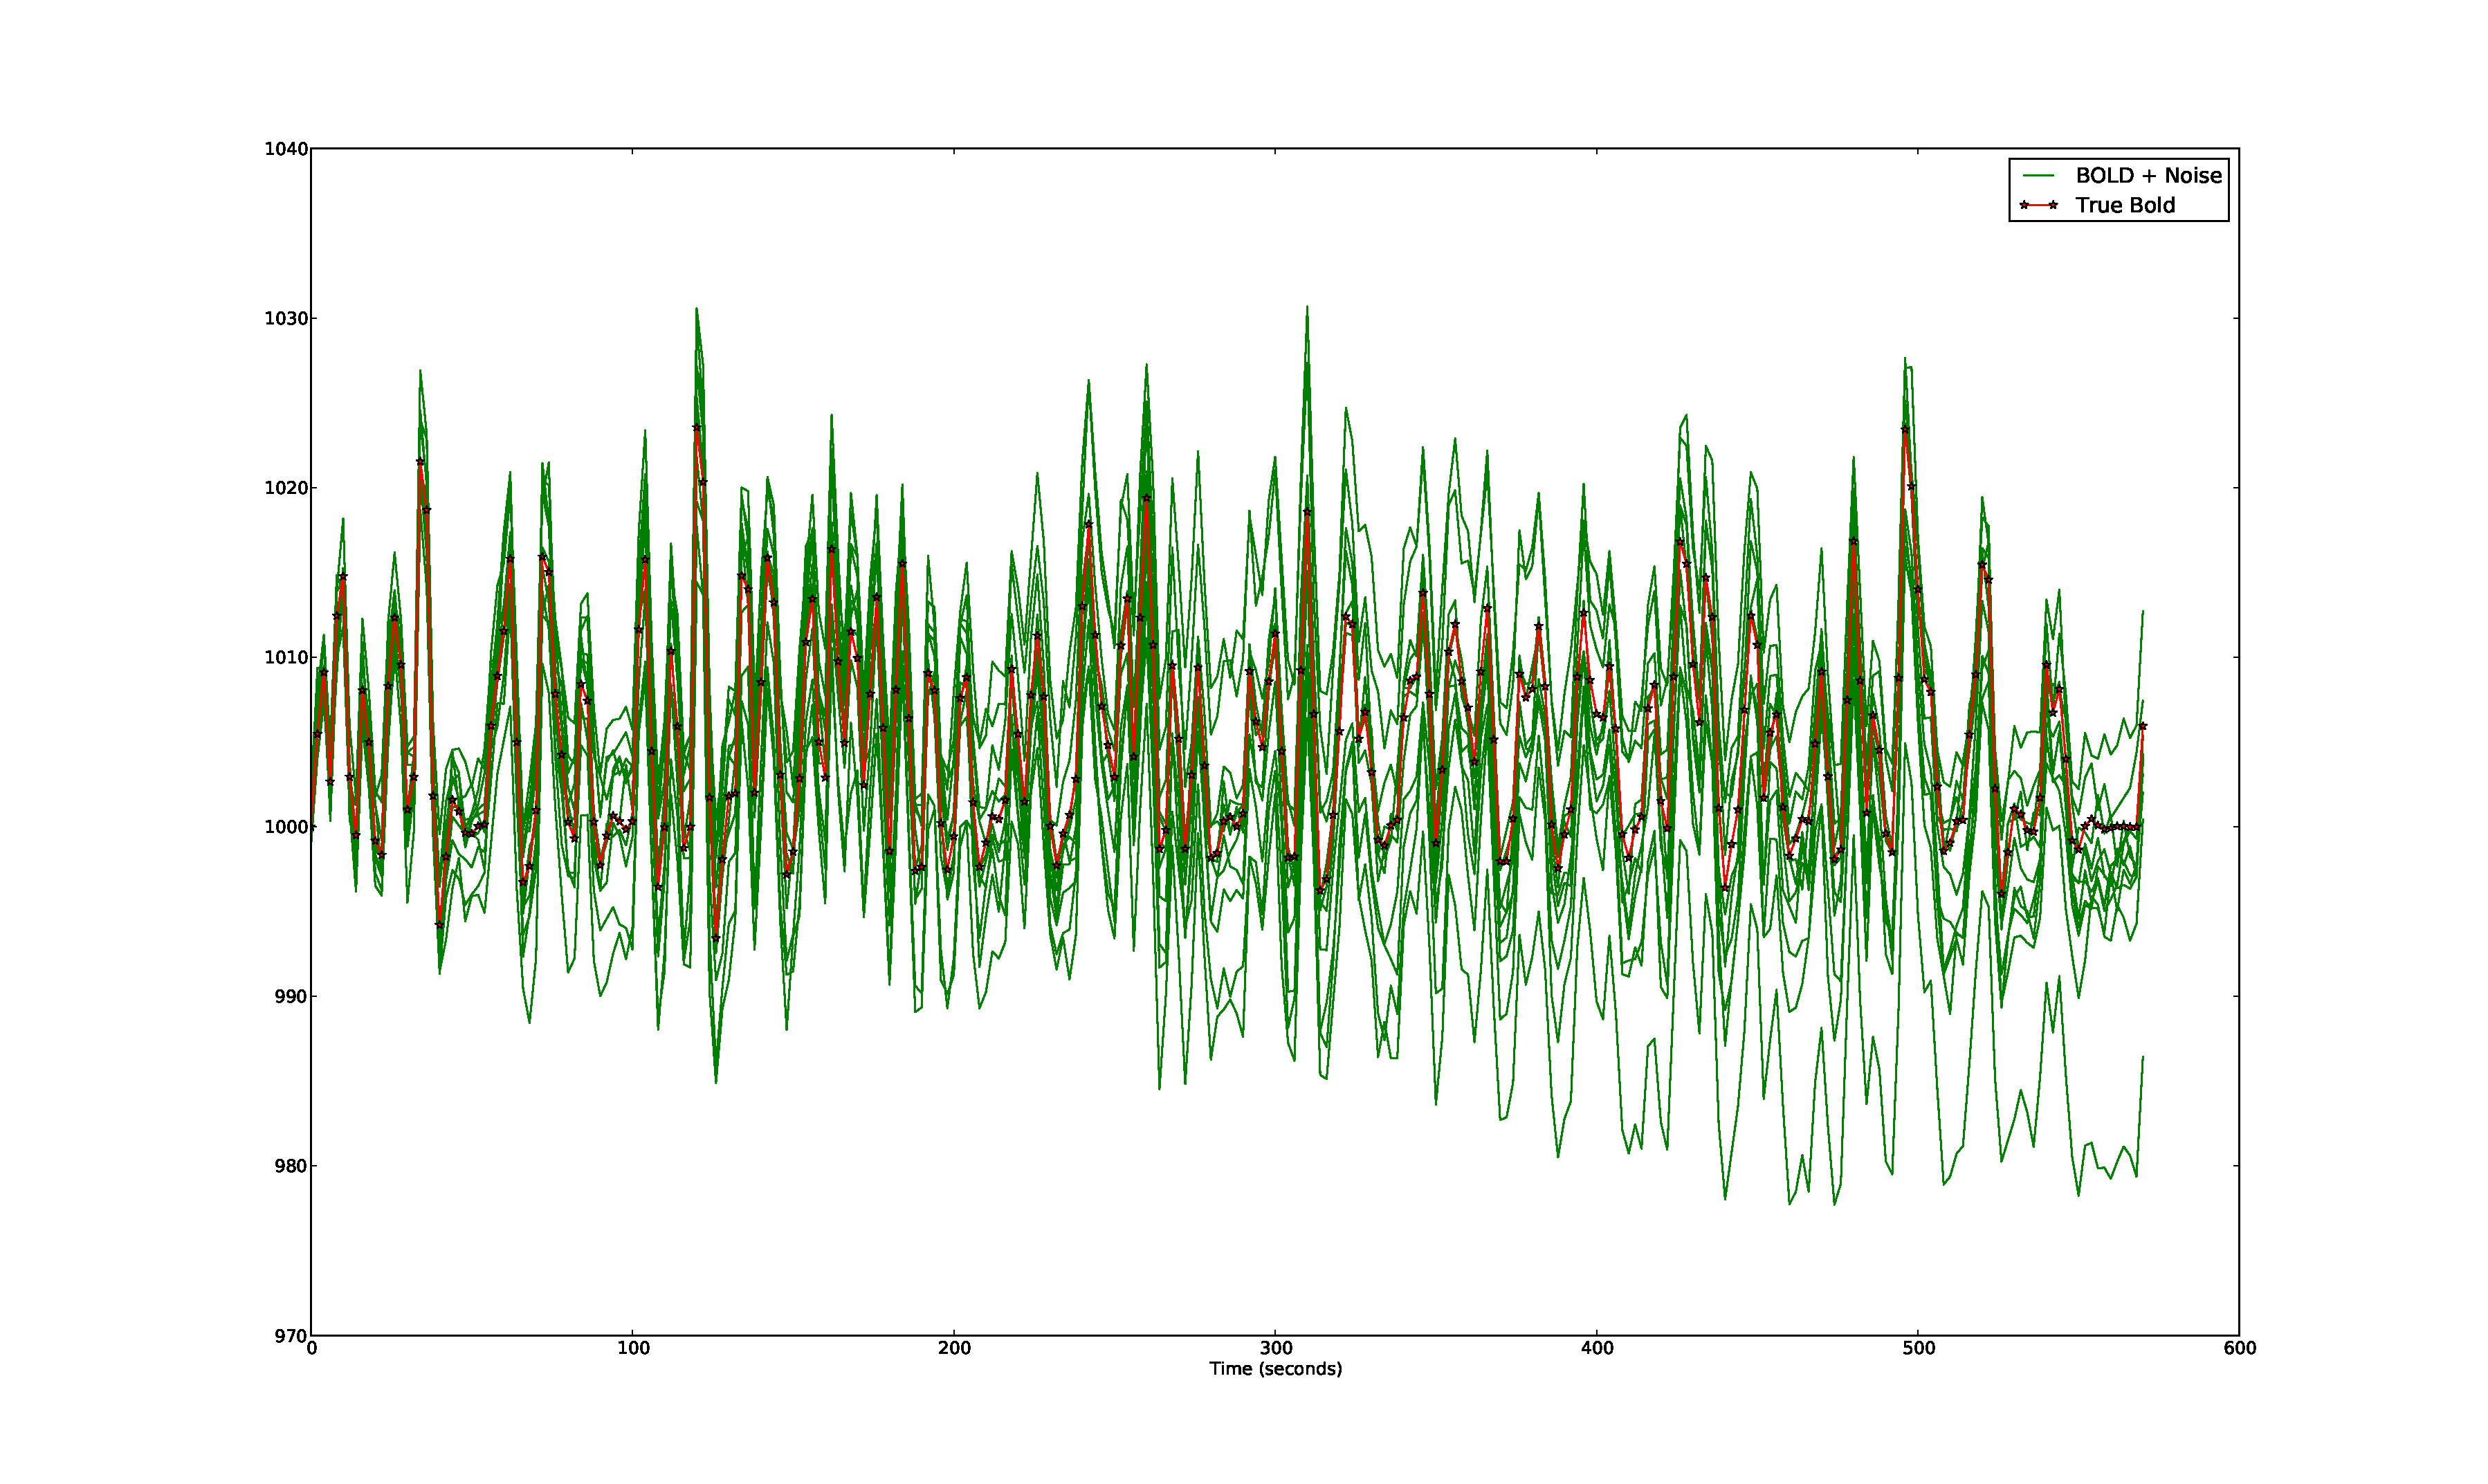
\includegraphics[clip=true,trim=6cm 2cm 6cm 3.5cm,width=7cm]{images/realization_lownoise}
\caption{Test Signals with low noise compared to the clean signal.}
\label{fig:LowNoiseRealization}
\end{figure}
\begin{figure}
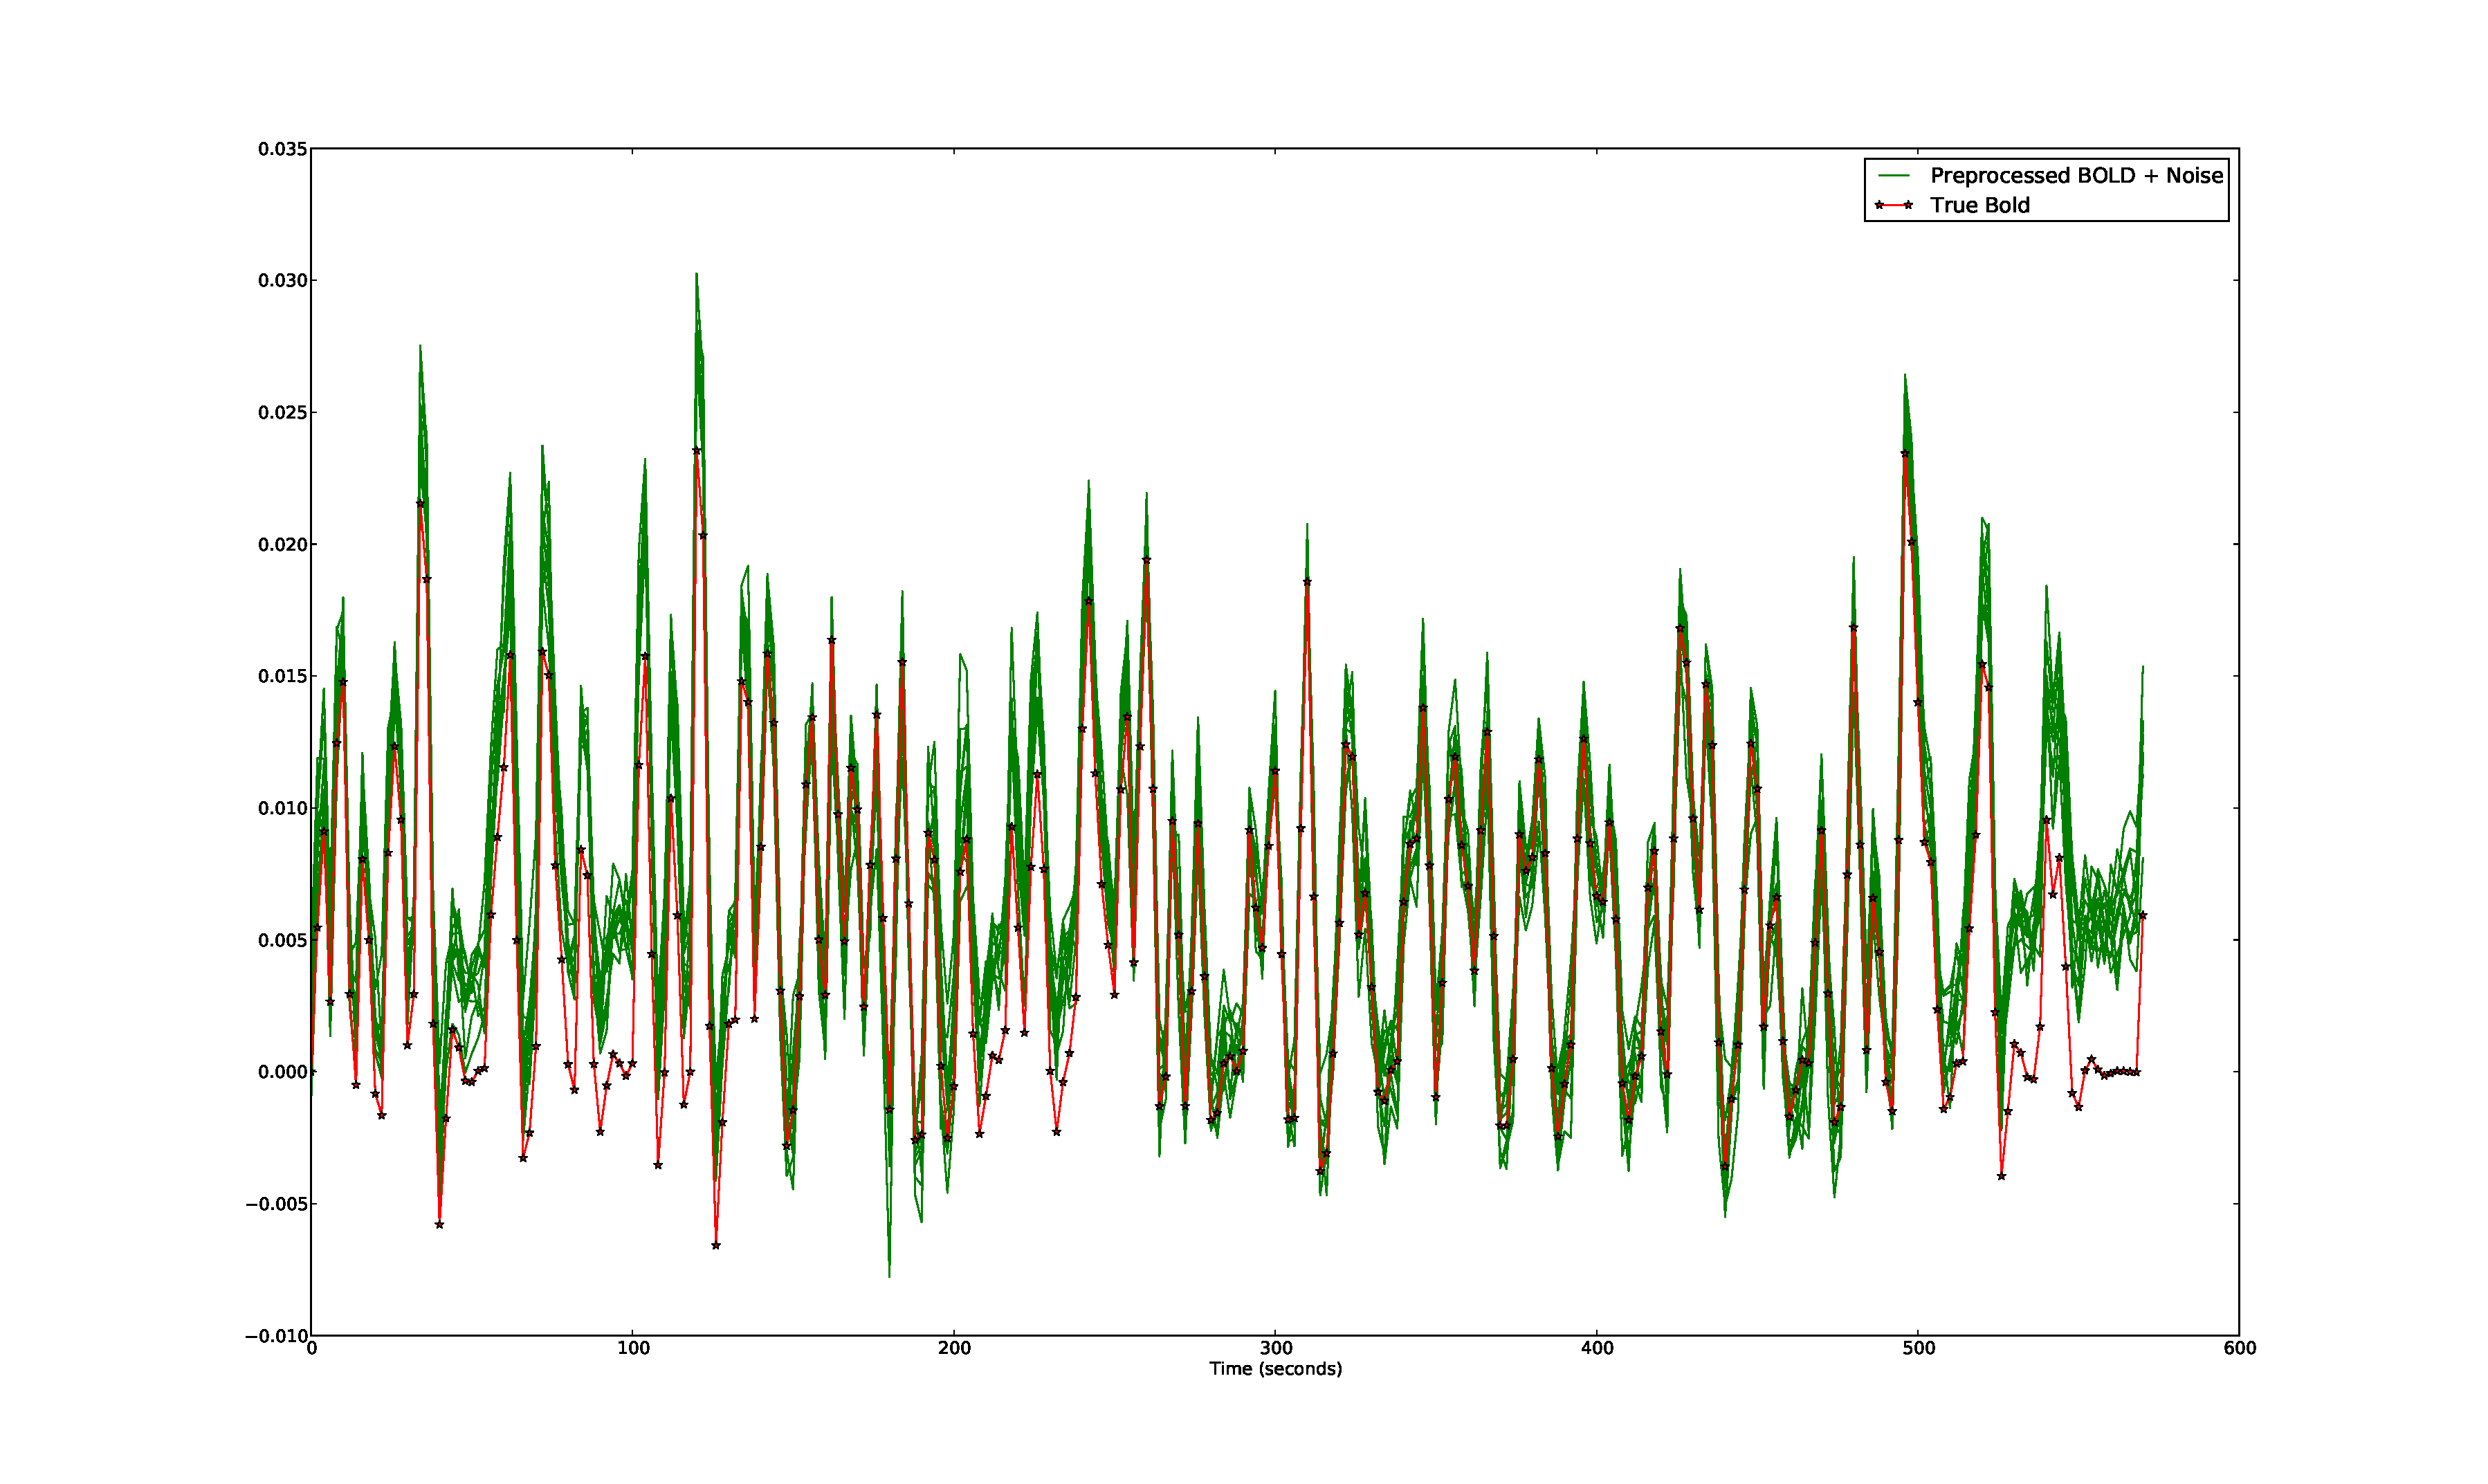
\includegraphics[clip=true,trim=6cm 2cm 6cm 3.5cm,width=7cm]{images/preprocessed_lownoise}
\caption{A comparison of the preprocessed signals for the low noise case. This is the
noisy input to the actual particle filter algorithm.}
\label{fig:PreprocessedLowNoise}
\end{figure}
\begin{figure}
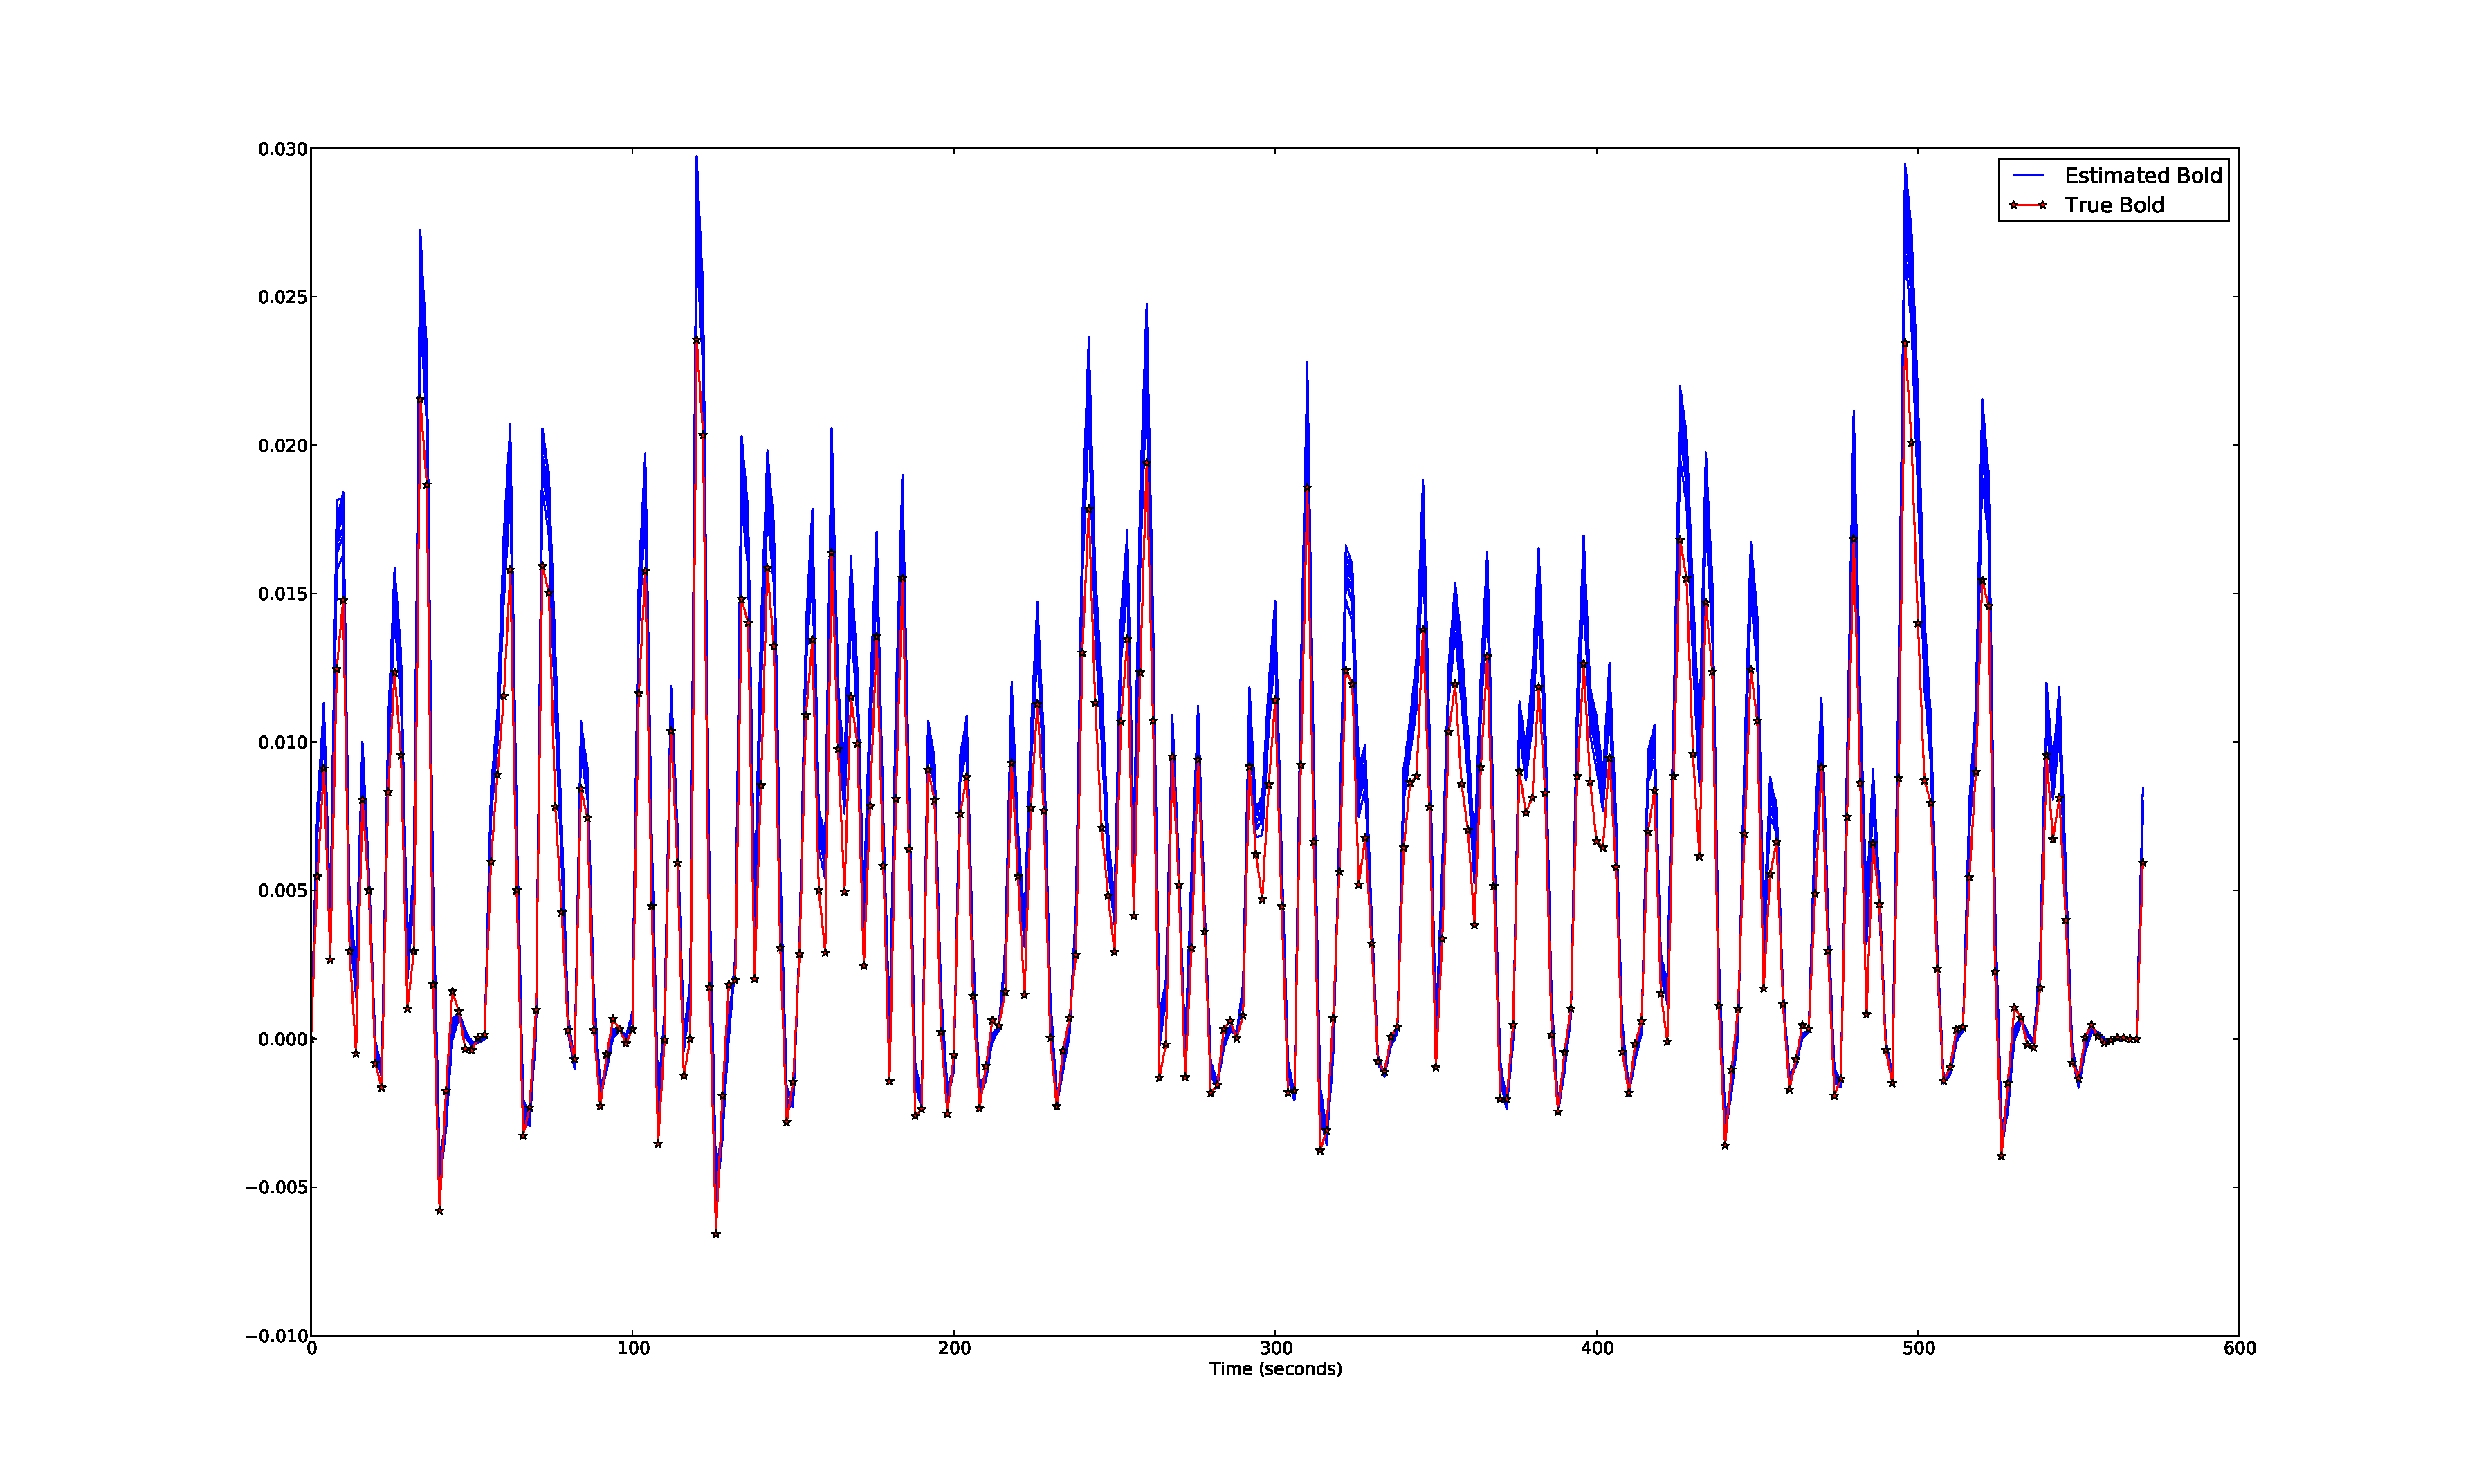
\includegraphics[clip=true,trim=6cm 2cm 6cm 3.5cm,width=17cm]{images/comparison_lownoise}
\caption{A comparison of the fitted signals for the low noise case.}
\label{fig:FitComparisonLowNoise}
\end{figure}

To begin the single voxel simulation; I generated a signal using the following parameters:
$\{\tau_0 = 1.45, \alpha = .3, E_0 = .47, V_0 = .044, \tau_s = 1.94, \tau_f = 1.99, \epsilon = 1.8\}$.
These same parameters were also used in the high noise case. The noise realizations were
then generated based on a measurement noise ($\sigma_y$) of $.001$ and a drift standard deviation
($\sigma_x$) of $.0005$. The measurement noise as well as the steps of the drift
were taken to be Gaussian
For this low noise case, the eleven realizations are shown in \autoref{fig:LowNoiseRealization}.
The actual signal delivered into the particle filter
was the result of some preprocessing to remove drift, as described in 
\autoref{sec:Methods Preprocessing}. The bias introduced into the signal by preprocessing 
may have some effect on the resulting fit; thus the preprocessed signal is compared
to the true BOLD signal in \autoref{fig:PreprocessedLowNoise}.
The preprocessing consists of several steps, which are discussed in detail in \autoref{sec:Methods Preprocessing}.
The data shows that the spline struggles to match the signal near the end, although 
overall, the preprocessing seems to have been successful at removing trends. Finally, the 
set of fits to the true BOLD signal are shown in \autoref{fig:FitComparisonLowNoise}.
The filtering property of the particle filter is clear from the results here.  In several locations the output
of the particle filter looks like a filtered version of the input. For instance toward the
end, the estimates stay flat in spite of the preprocessed data drifting off. By
this point, the algorithm has converged sufficiently to know that that such a movement in
signal isn't possible. A similar circumstance occurs at 100 seconds in. 
It is also worth noting the bias introduced by pre-processing 
results in a slightly larger peak signal. The final parameter sets are shown in 
\autoref{tab:LowNoiseResults}. Note that throughout the results, unless otherwise specified,
the residual will be defined as the square root of the mean squared residual, 
\begin{equation}
\text{Residual} = \sqrt{\sum (\hat{y}_k - y_k)^2}
\end{equation}
where $\hat{y}_k$ is the estimated output at time $k$ and $y_k$ is the output
sample at time $k$. Note the subtle distinction between this and the error
which is defines as 
\begin{equation}
\text{Error} = \sqrt{\sum (\hat{y}_k - Y_k)^2}
\end{equation}
where $\hat{y}_k$ is the estimated output, and $Y_k$ is the underlying (free of noise)
output. Throughout this section and the next, the terms \emph{error} and \emph{residual}
will be referencing these values, for an entire timeseries.

\begin{table}[t]
\centering
\begin{tabular}{|c | c | c | c | c | c | c | c | c | c |}
\hline 
$\tau_0$ & $\alpha$ & $E_0$    & $V_0$    & $\tau_s$ & $\tau_f$ & $\epsilon$  & $ \sum \tau $ & $\sqrt{MSR}$ &$\sqrt{MSE}$\\
\hline 
\rowcolor[gray]{.8}
1.45 & .3 & .47 & .044 & 1.94 & 1.99 & 1.8  & 5.38 &  & \\
\hline 
\hline 
1.2221 & 0.3449 & 0.3346 & 0.0714 & 1.6045 & 2.2753 & 1.5945 & 5.1019 &  0.003211  & 0.009876  \\
1.3749 & 0.3318 & 0.3630 & 0.0733 & 1.6408 & 2.1030 & 1.5763 & 5.1187 &  0.003055  & 0.009932  \\
1.1660 & 0.3221 & 0.3406 & 0.0822 & 1.6477 & 2.3535 & 1.2452 & 5.1672 &  0.003289  & 0.009680  \\
1.2318 & 0.3271 & 0.3403 & 0.0796 & 1.6270 & 2.1852 & 1.3033 & 5.0439 &  0.002847  & 0.009120  \\
1.1832 & 0.3179 & 0.3472 & 0.0821 & 1.5496 & 2.2912 & 1.2782 & 5.0240 &  0.003006  & 0.009713  \\
1.1424 & 0.334  & 0.3473 & 0.0737 & 1.6221 & 2.2908 & 1.4025 & 5.0553 &  0.002833  & 0.009485  \\
1.3004 & 0.3596 & 0.3564 & 0.0768 & 1.5641 & 2.1323 & 1.6034 & 4.9968 &  0.003028  & 0.010219  \\
1.2401 & 0.3460 & 0.3398 & 0.0891 & 1.6499 & 2.2366 & 1.2900 & 5.1265 &  0.003044  & 0.010080  \\
1.1709 & 0.3274 & 0.3464 & 0.0826 & 1.5373 & 2.2826 & 1.3783 & 4.9909 &  0.003345  & 0.010329  \\
1.1897 & 0.3434 & 0.3355 & 0.0798 & 1.5358 & 2.3075 & 1.4277 & 5.0330 &  0.003175  & 0.010015  \\
1.184 &  0.3405 & 0.3502 & 0.0892 & 1.6103 & 2.2793 & 1.1645 & 5.0735 &  0.002889  & 0.009505  \\
\hline                                                                           
1.2187 & 0.3359 & 0.3456 & 0.0800 & 1.599 & 2.2488 & 1.3876 & 5.0665 & 0.003066     & 0.009814 \\
\hline 
\end{tabular}
\caption{Estimated Parameters on 11 different runs with low noise. First row is the true parameters,
last is mean over the 11 runs. The $\sqrt{MSR}$ is residual and $\sqrt{MSE}$ is the error.}
\label{tab:LowNoiseResults} 
\end{table}

\begin{table}[t]
\centering
\begin{tabular}{|c | c  c  c  c  c  c  c |}
\hline 
  & $\tau_0$ & $\alpha$ & $E_0$    & $V_0$    & $\tau_s$ & $\tau_f$ & $\epsilon$ \\
\hline 
\rowcolor[gray]{.8} $\tau_0$ &   0.0189481 & -0.0014269 & -0.0011267 & -1.13e-05 & -0.0025616 & -0.0189559 & 0.0070405 \\
$\alpha$ &                       -0.0014269 & 0.0026716 & 9.93e-05 & -0.0002041 & -0.0008632 & -0.0016823 & 0.0071891 \\
\rowcolor[gray]{.8} $E_0$    &   -0.0011267 & 9.93e-05 & 0.0010701 & -0.0002277 & -0.0001177 & 0.0001013 & 0.0016972 \\
$V_0$    &                       -1.13e-05 & -0.0002041 & -0.0002277 & 0.0005401 & 4.3e-06 & 4.56e-05 & -0.0080494 \\
\rowcolor[gray]{.8} $\tau_s$ &   -0.0025616 & -0.0008632 & -0.0001177 & 4.3e-06 & 0.0128056 & 0.012878 & -0.005516 \\
$\tau_f$ &                       -0.0189559 & -0.0016823 & 0.0001013 & 4.56e-05 & 0.012878 & 0.0416927 & -0.0158182 \\
\rowcolor[gray]{.8} $\epsilon$&  0.0070405 & 0.0071891 & 0.0016972 & -0.0080494 & -0.005516 & -0.0158182 & 0.1567165 \\
\hline 
\end{tabular}
\caption{Typical Covariance matrix of the parameters at the end of a run.}
\label{tab:CovSim} 
\end{table}

\begin{figure}
\subfigure[Converging histogram for $\tau_0$, $\alpha$, $E_0$, and $V_0$ of the first run, low noise simulation.]
{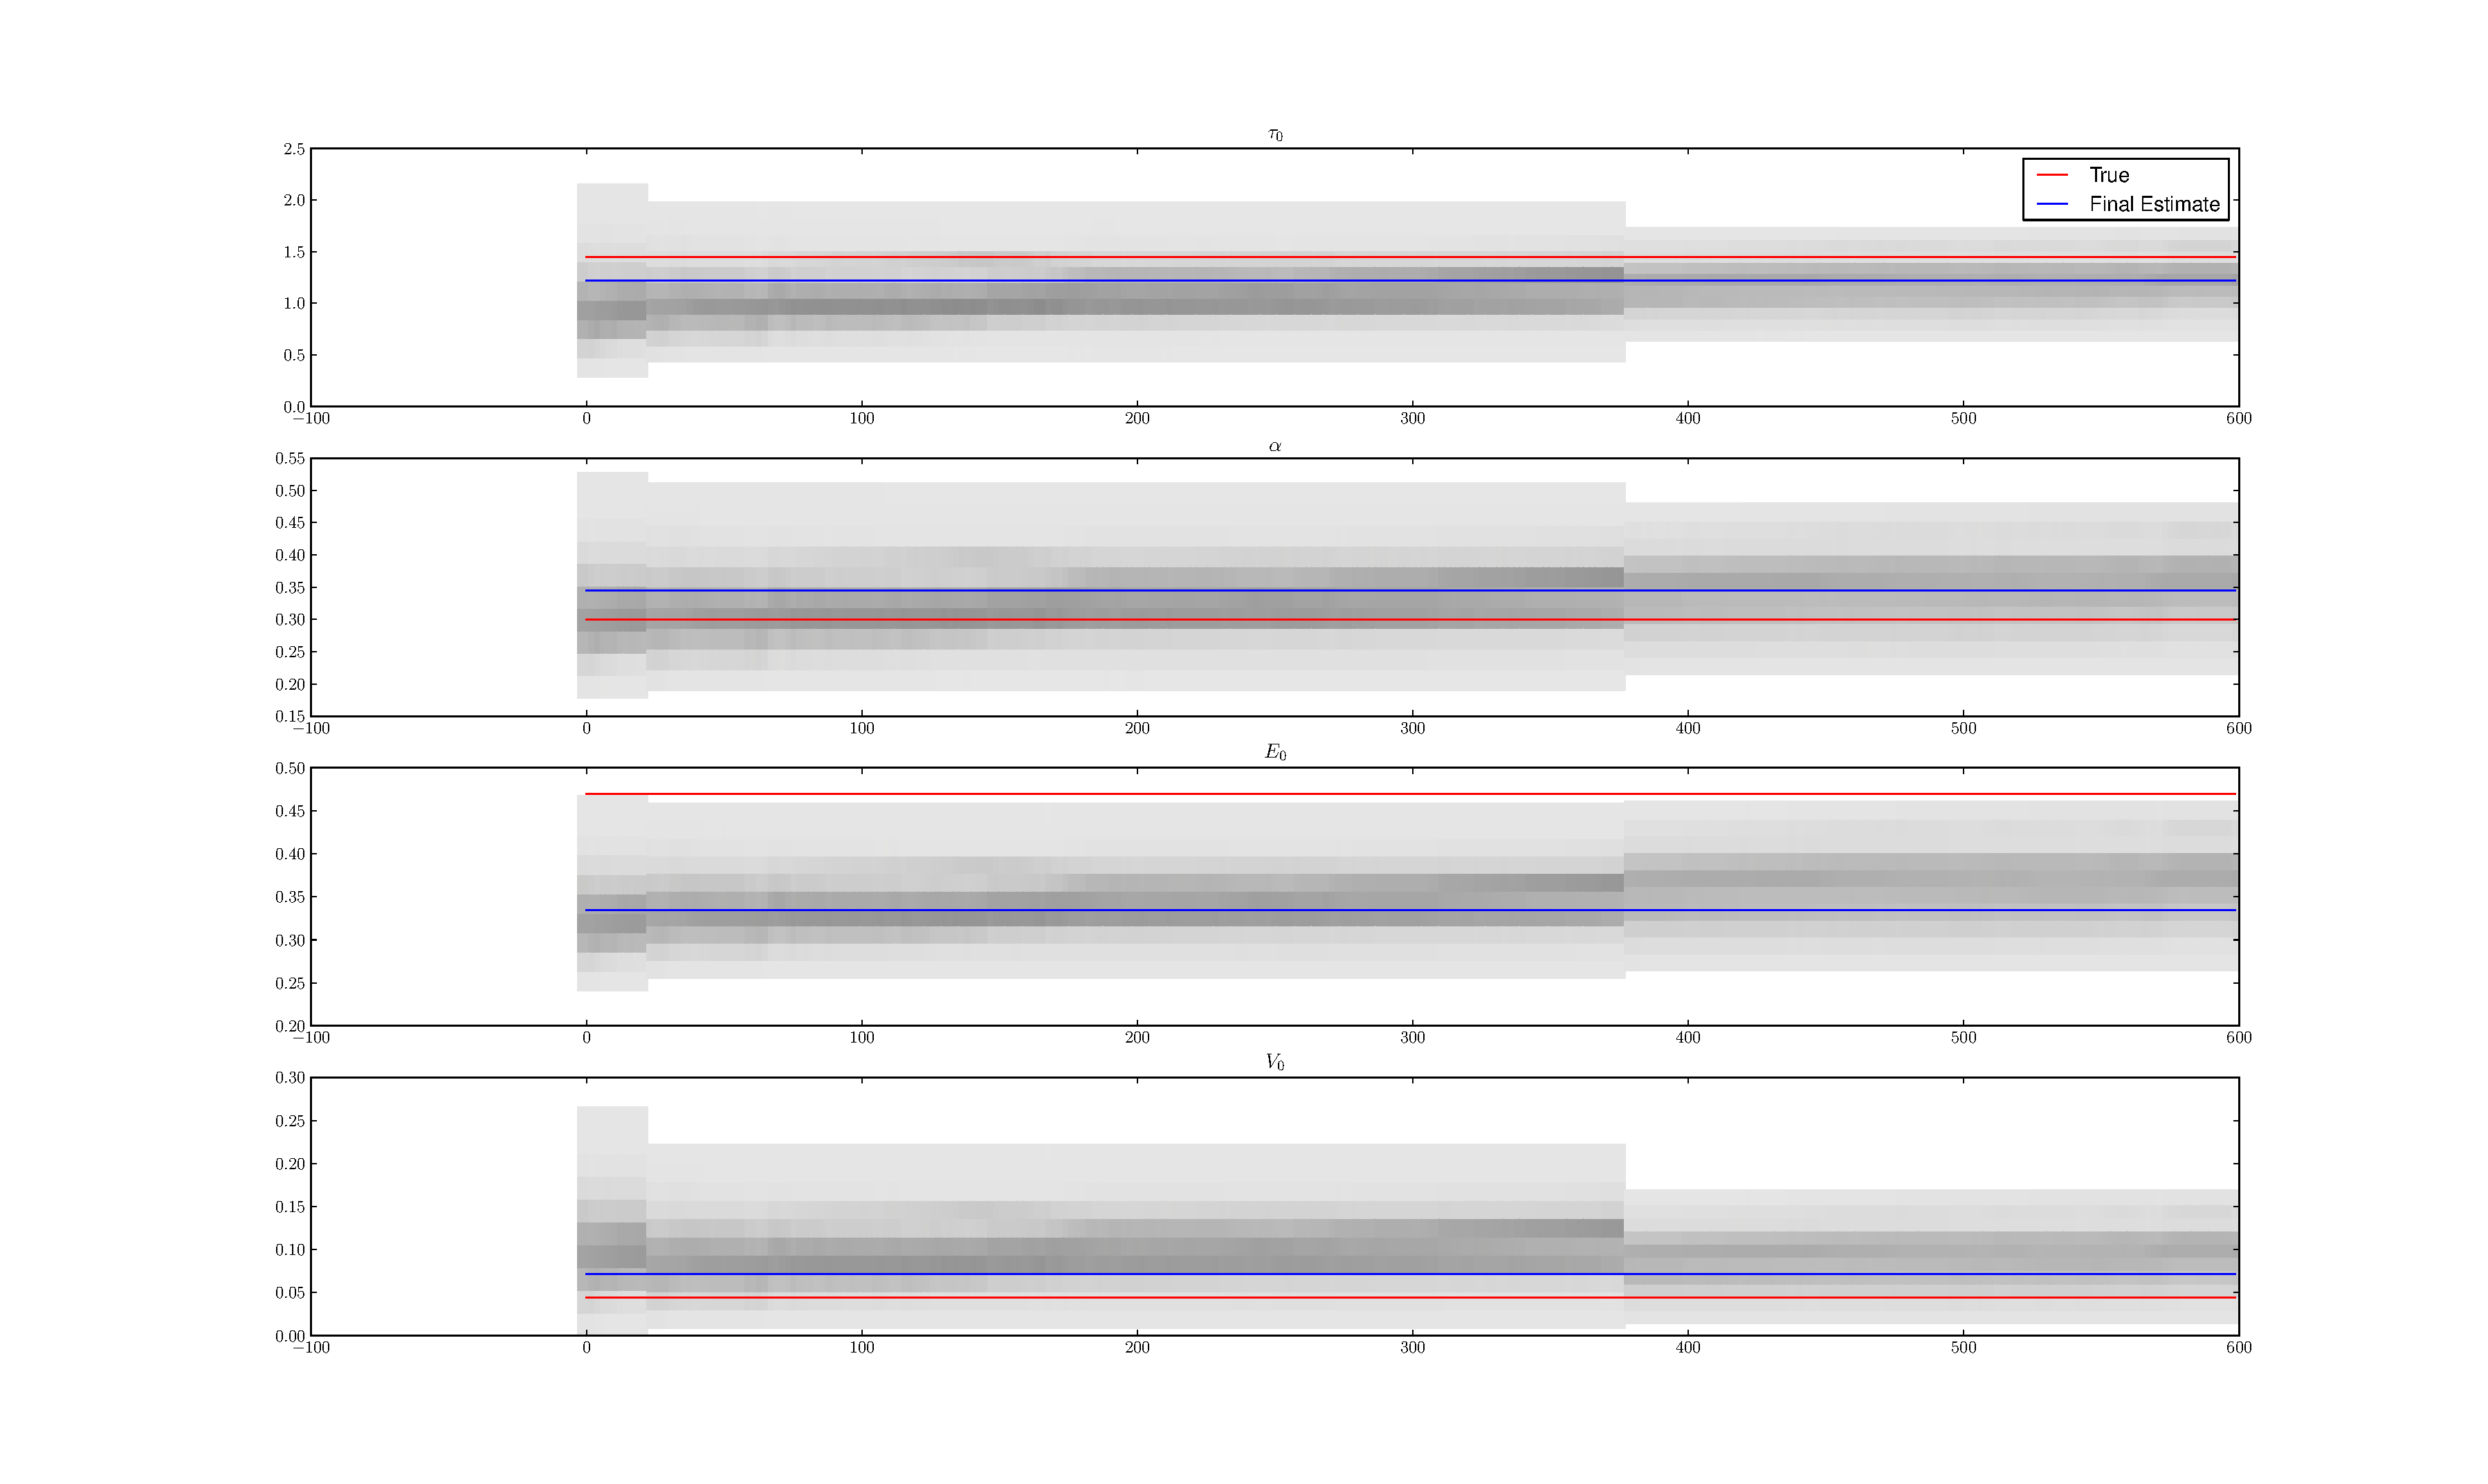
\includegraphics[clip=true,trim=7cm 3cm 6cm 3cm, width=16cm]{images/converge_lownoise1}}\\

\subfigure[Converging histogram for $\tau_s$, $\tau_f$, $\epsilon$, and $V$ of the first run, low noise simulation.]
{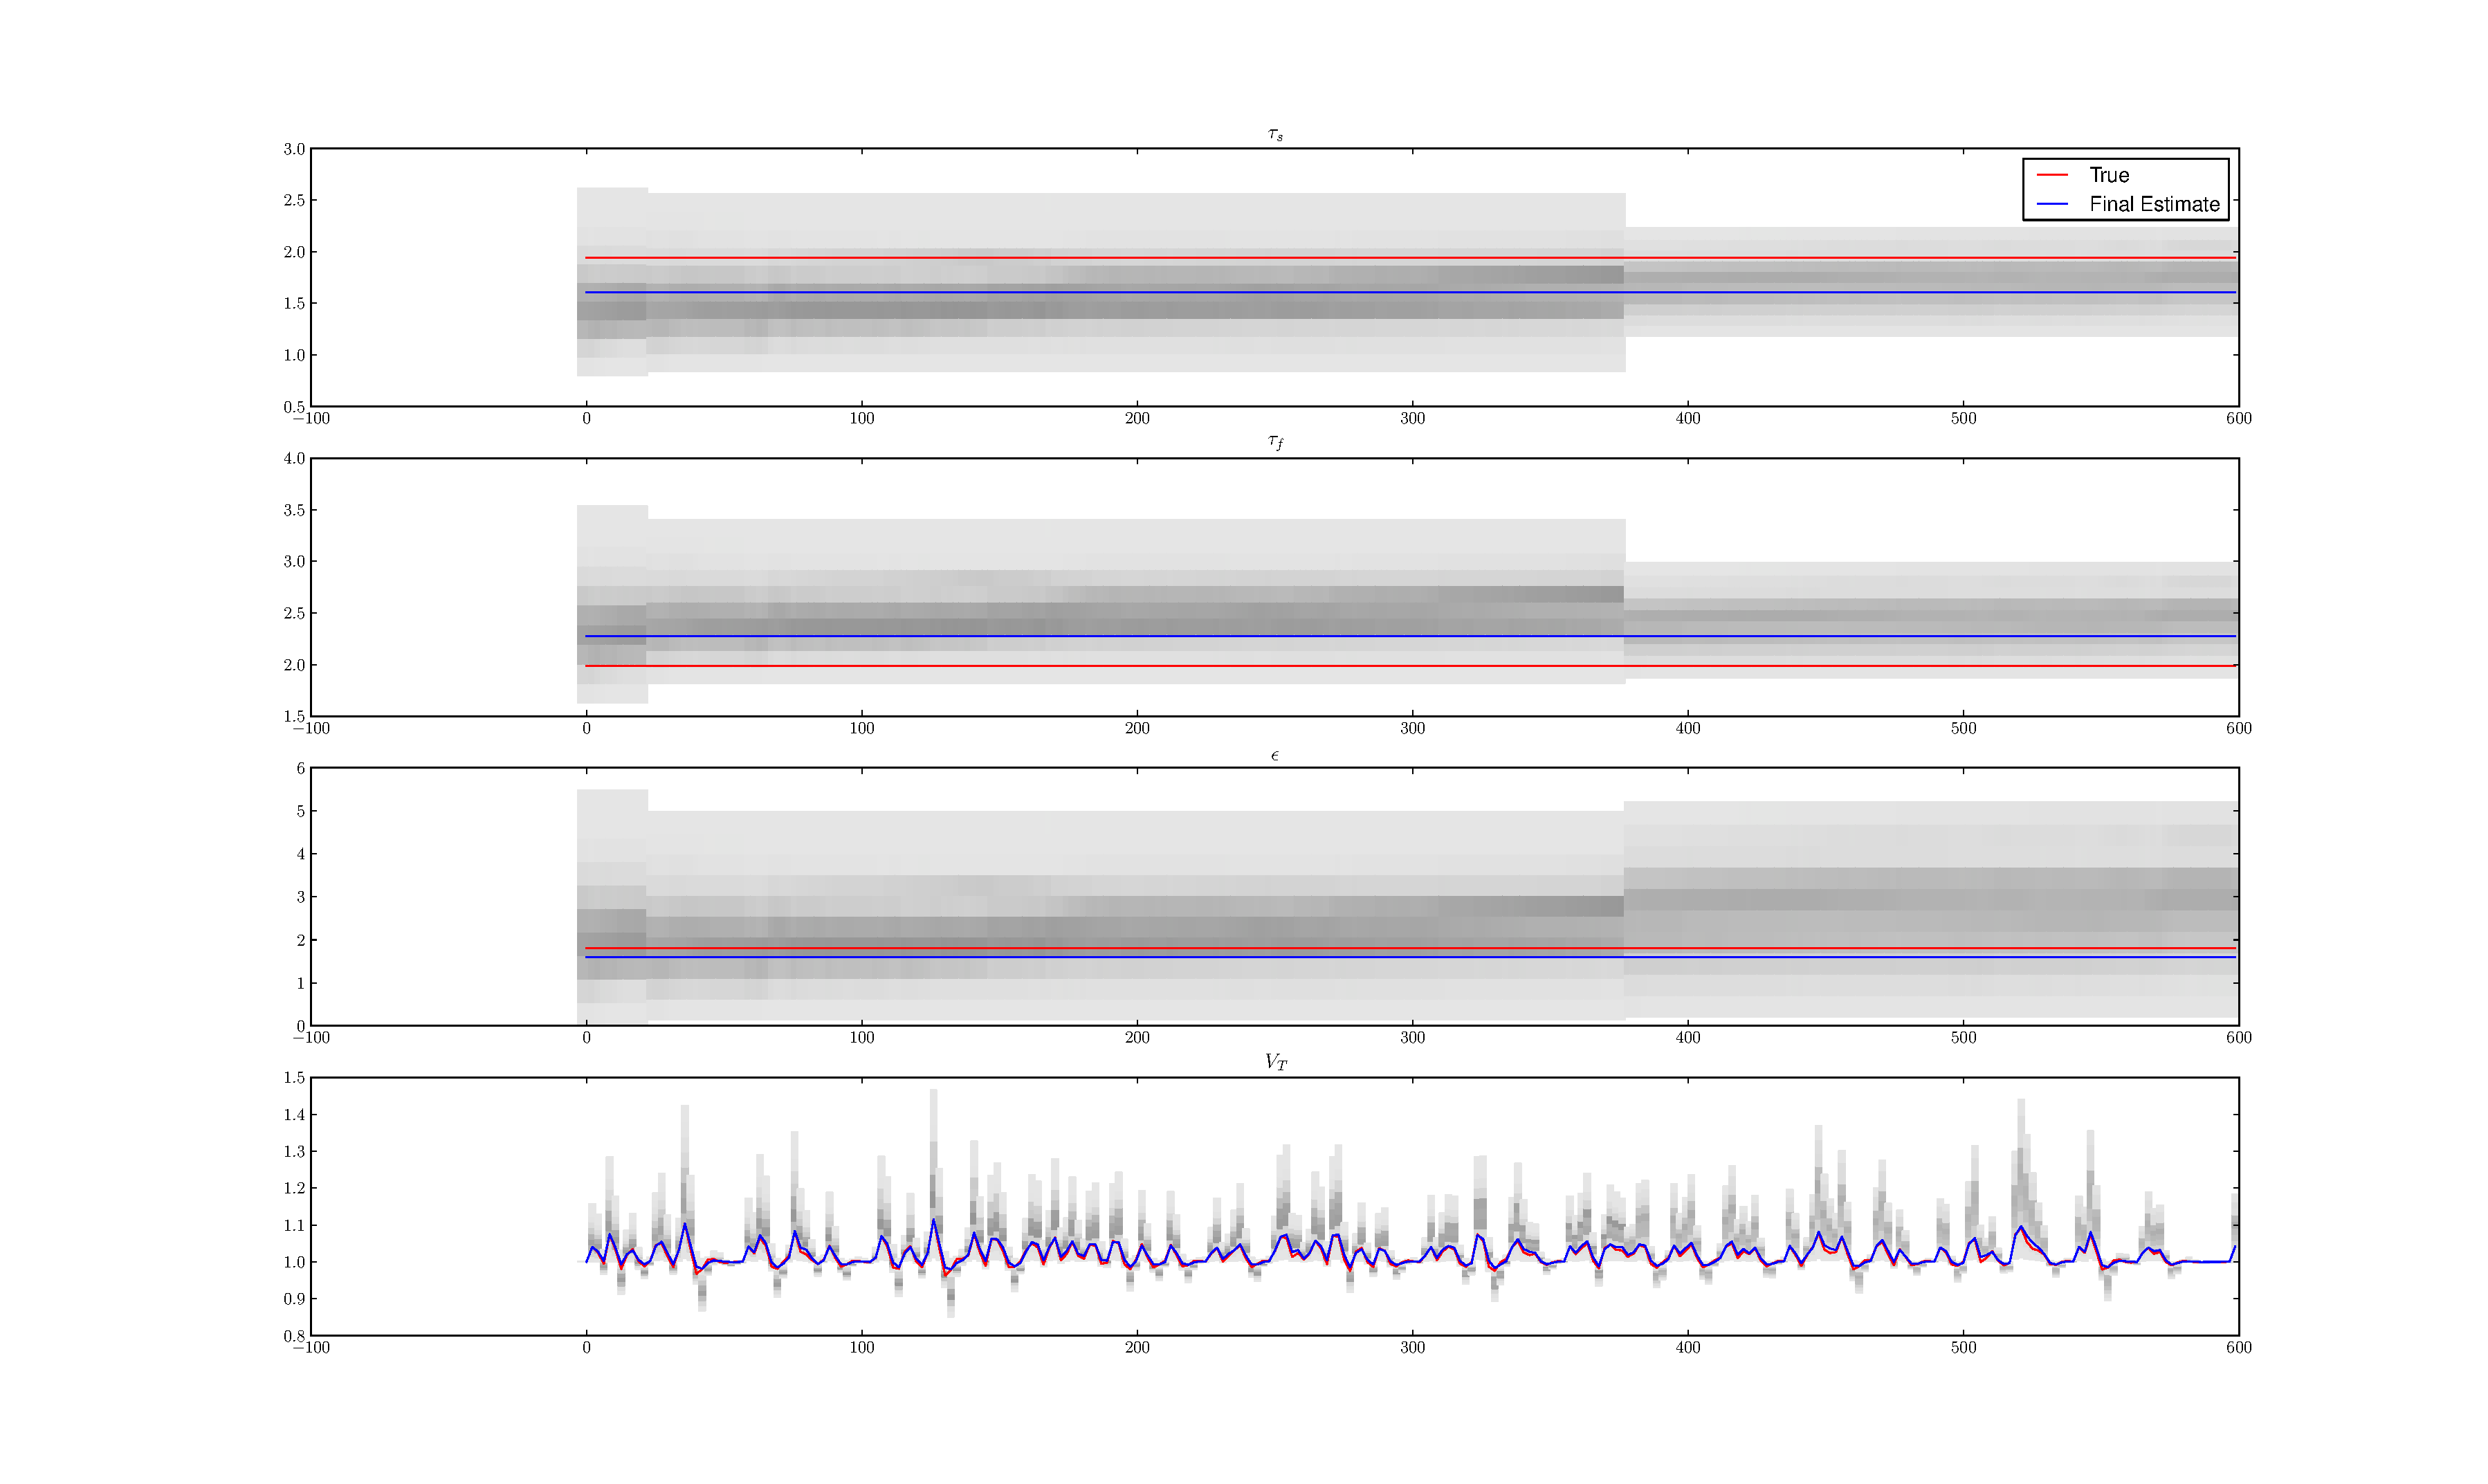
\includegraphics[clip=true,trim=7cm 3cm 6cm 3cm, width=16cm]{images/converge_lownoise2}}\\
\end{figure}

\begin{figure}
\subfigure[Converging histogram for $Q$, $S$, $F$, and $BOLD$ of the first run, low noise simulation.]
{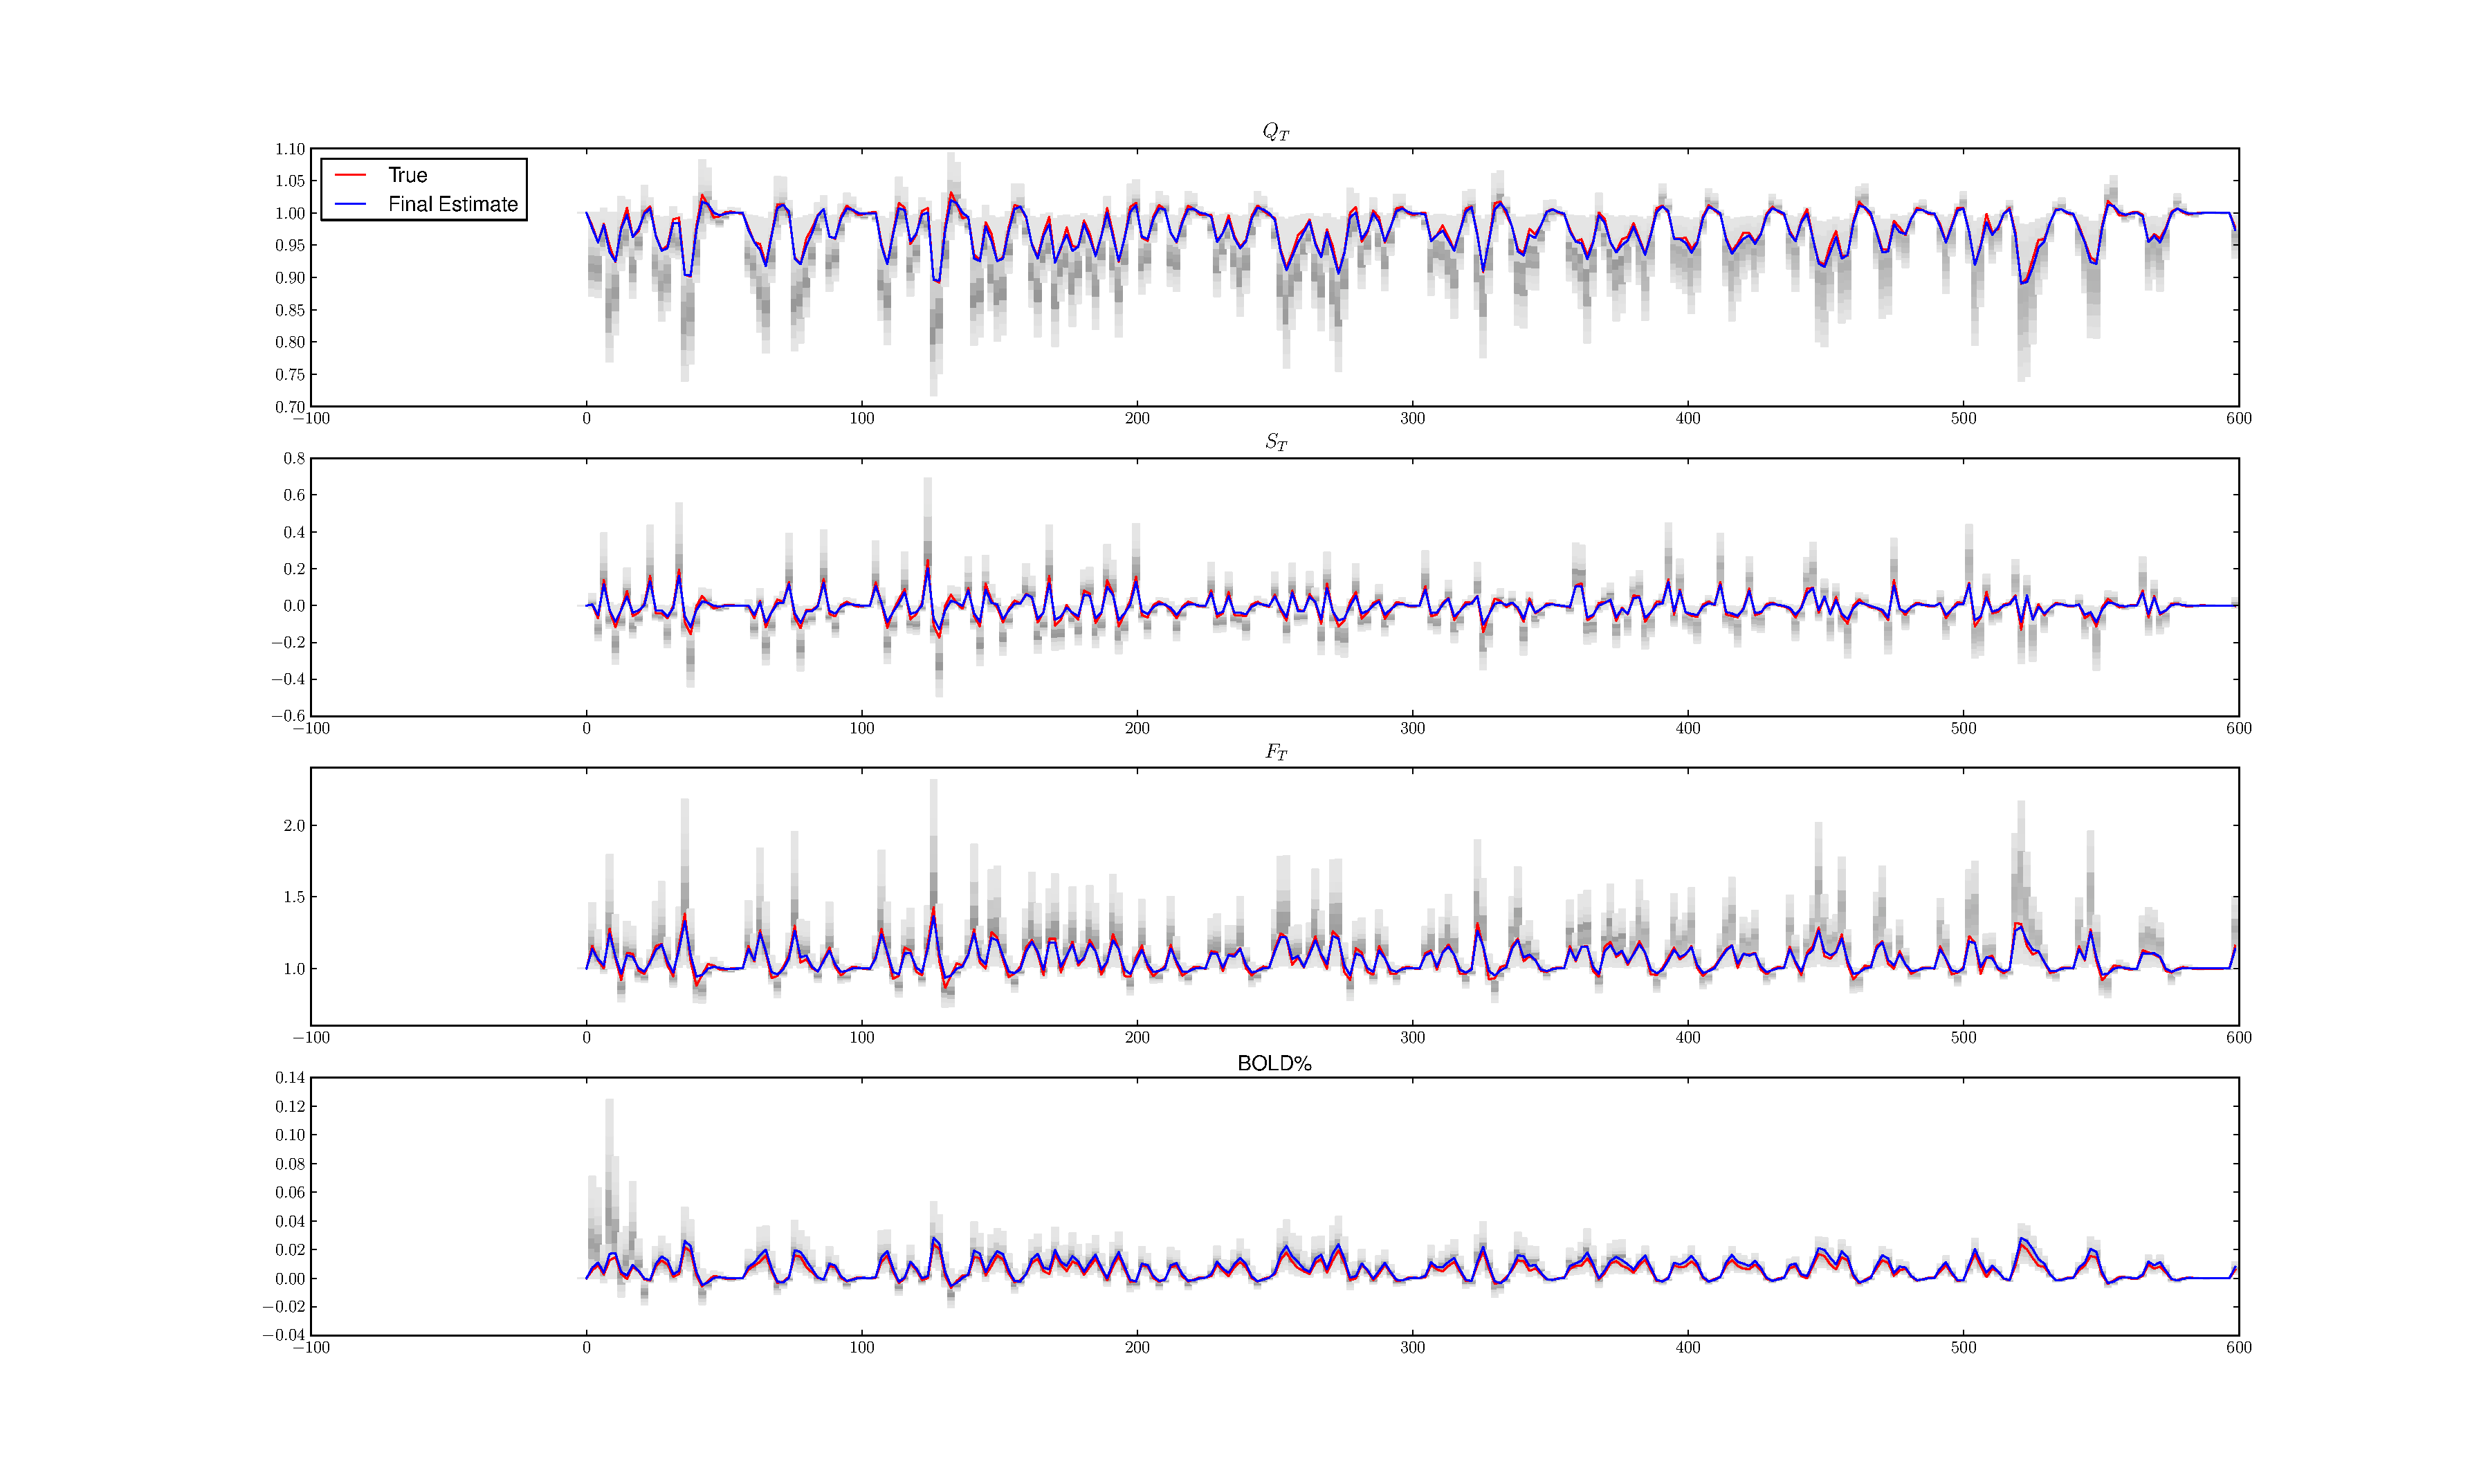
\includegraphics[clip=true,trim=7cm 3cm 6cm 3cm, width=16cm]{images/converge_lownoise3}}
\label{fig:LowNoiseHist}
\end{figure}

There are a few results worth noting in the final parameter estimates (which 
are the mean of the particle filter's posterior distribution). First the time constants vary 
greatly across
runs with different noise realizations, yet the sum of the individual time constants
($\tau_f$, $\tau_s$ and $\tau_0$) seems to be more consistent. In general the 
time constants fall short of the true time constant. This could be a limitation
based on the prior distribution (which notably has an initial mean below the true values) 
or it could be caused by the disassociated benefits of a correct time
constant with regards to a correct output. It often takes several measurement periods before 
a difference
in time constants becomes relevant to the weight. Its also possible that output is insensitive
to differences in the time constants; althouhg varying the activation durations could induce
better estimates.  The large variation of $V_0$ are also interesting, although as one final
covariance matrix shows, there is a definite negative correlation between $\epsilon$ and $V_0$.
In general,
with this admittedly small amount of noise, it would appear that the relation between a set
of parameters/stimuli and the output is not injective; a time
series is not unique to a single set of parameters. This is good justification that 
simultaneous blood volume or tagged flow calculations with the conventional FMRI 
could benefit the model. 

The covariance matrix (\autoref{tab:CovSim}) provides a great deal of insight into 
the way parameters evolve in the particle filter. The fact that there are so many 
covariance elements that are as big or bigger than variance elements indicates just
loose the parameters set is. Every single parameters, including $\alpha$ seems to
have a non-zero covariance. Why $\alpha$ and $\epsilon$ would be positively related
is one of the most interesting element. Given the difficulty in mapping out a 
seven dimensional space, it is difficult to know why such correlations exist. 
 Notice the covariance of $\tau_f$ and $\tau_0$
is $-0.019$ whereas
the variance of $\tau_0$ and $\tau_f$ are $0.019$ and $0.04$ respectively. Clearly there is 
some measure of ill-defined behavior between the different time-constants, which is to
be expected given the number steps before a stimuli affects the output. 
The convergence properties of the first run in \autoref{tab:LowNoiseResults} 
demonstrates the migration of parameters to match the estimates. Given the relatively high
variance of parameters, its likely that more measurements or perhaps more variation
in the stimuli could further differentiate the parameters. Its also notable that
the final mean of the parameters may not be the best point estimator, and that perhaps
using the mode would be a better way to estimate the output. Regardless, the time series'
generated from the estimated mean seems to match the correct signal very well 
(\autoref{fig:FitComparisonLowNoise}).

%HIGH NOISE SECTION, with a signal
\subsection{High Noise}
\label{sec:HighNoise}
\begin{figure}
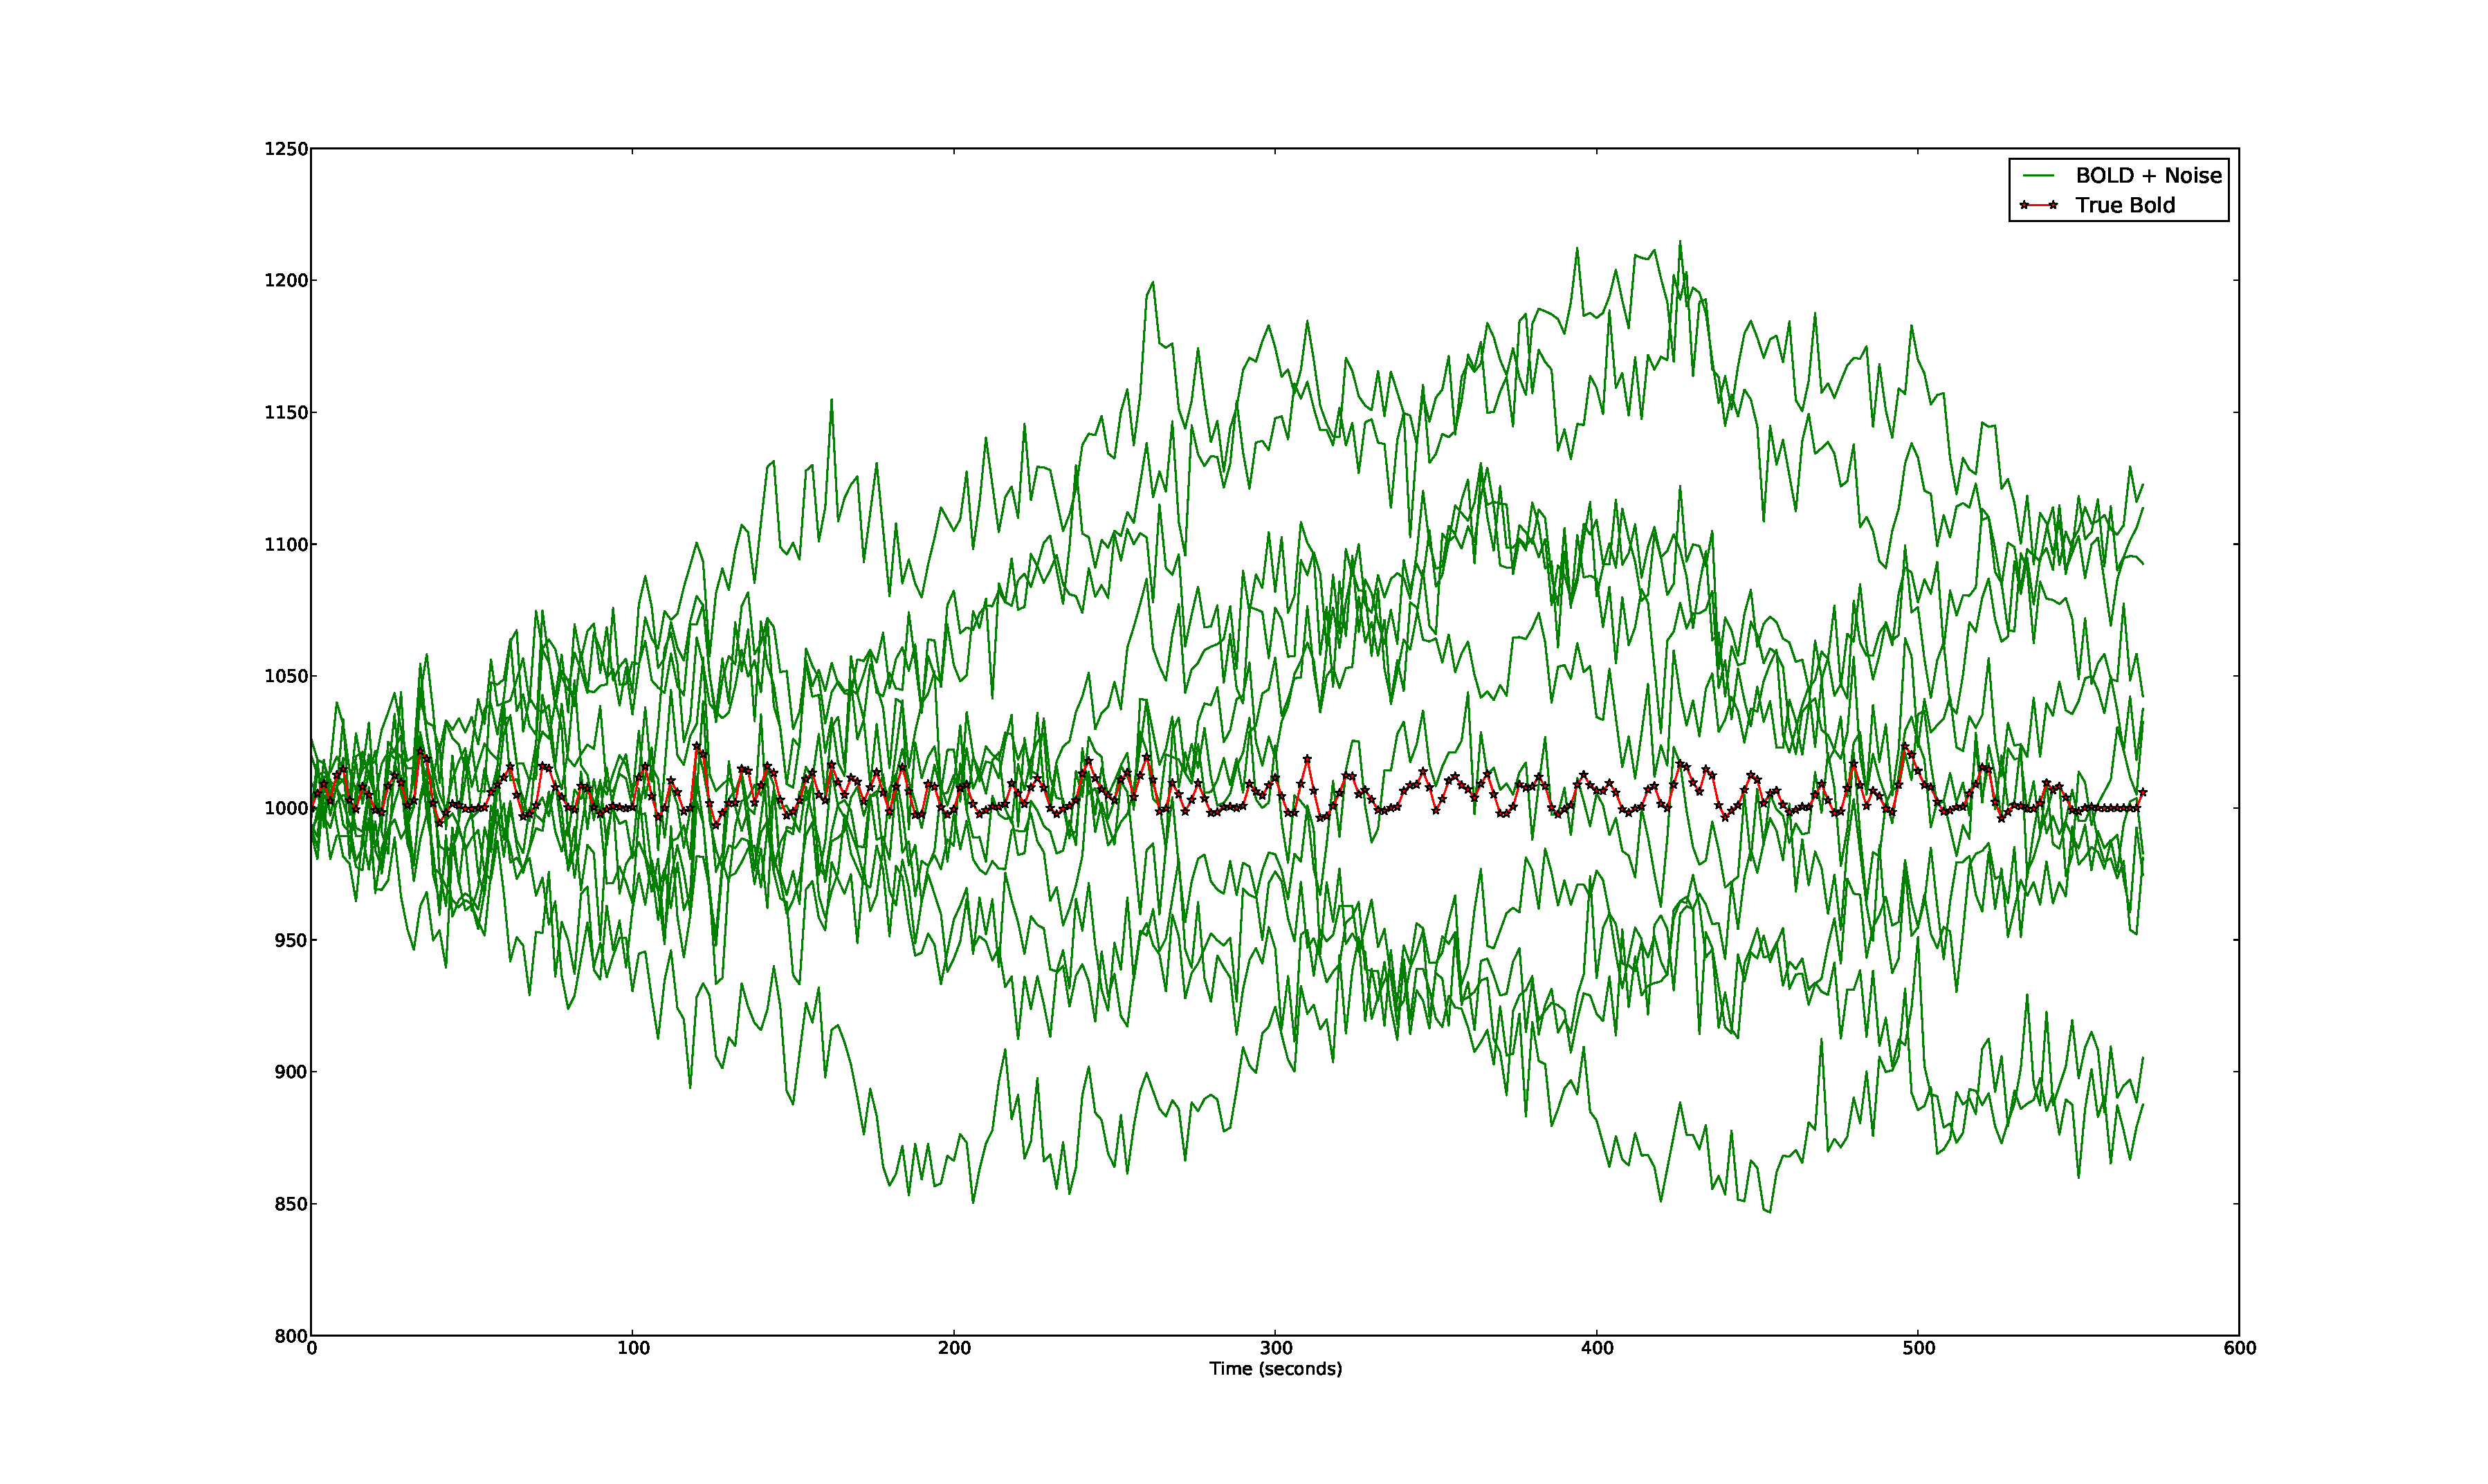
\includegraphics[clip=true,trim=6cm 2cm 6cm 3.5cm,width=7cm]{images/realization_highnoise}
\caption{Test Signals with high noise compared to the clean signal, $\sigma_x = .01, \sigma_y=.005$}
\label{fig:HighNoiseRealization}
\end{figure}
\begin{figure}
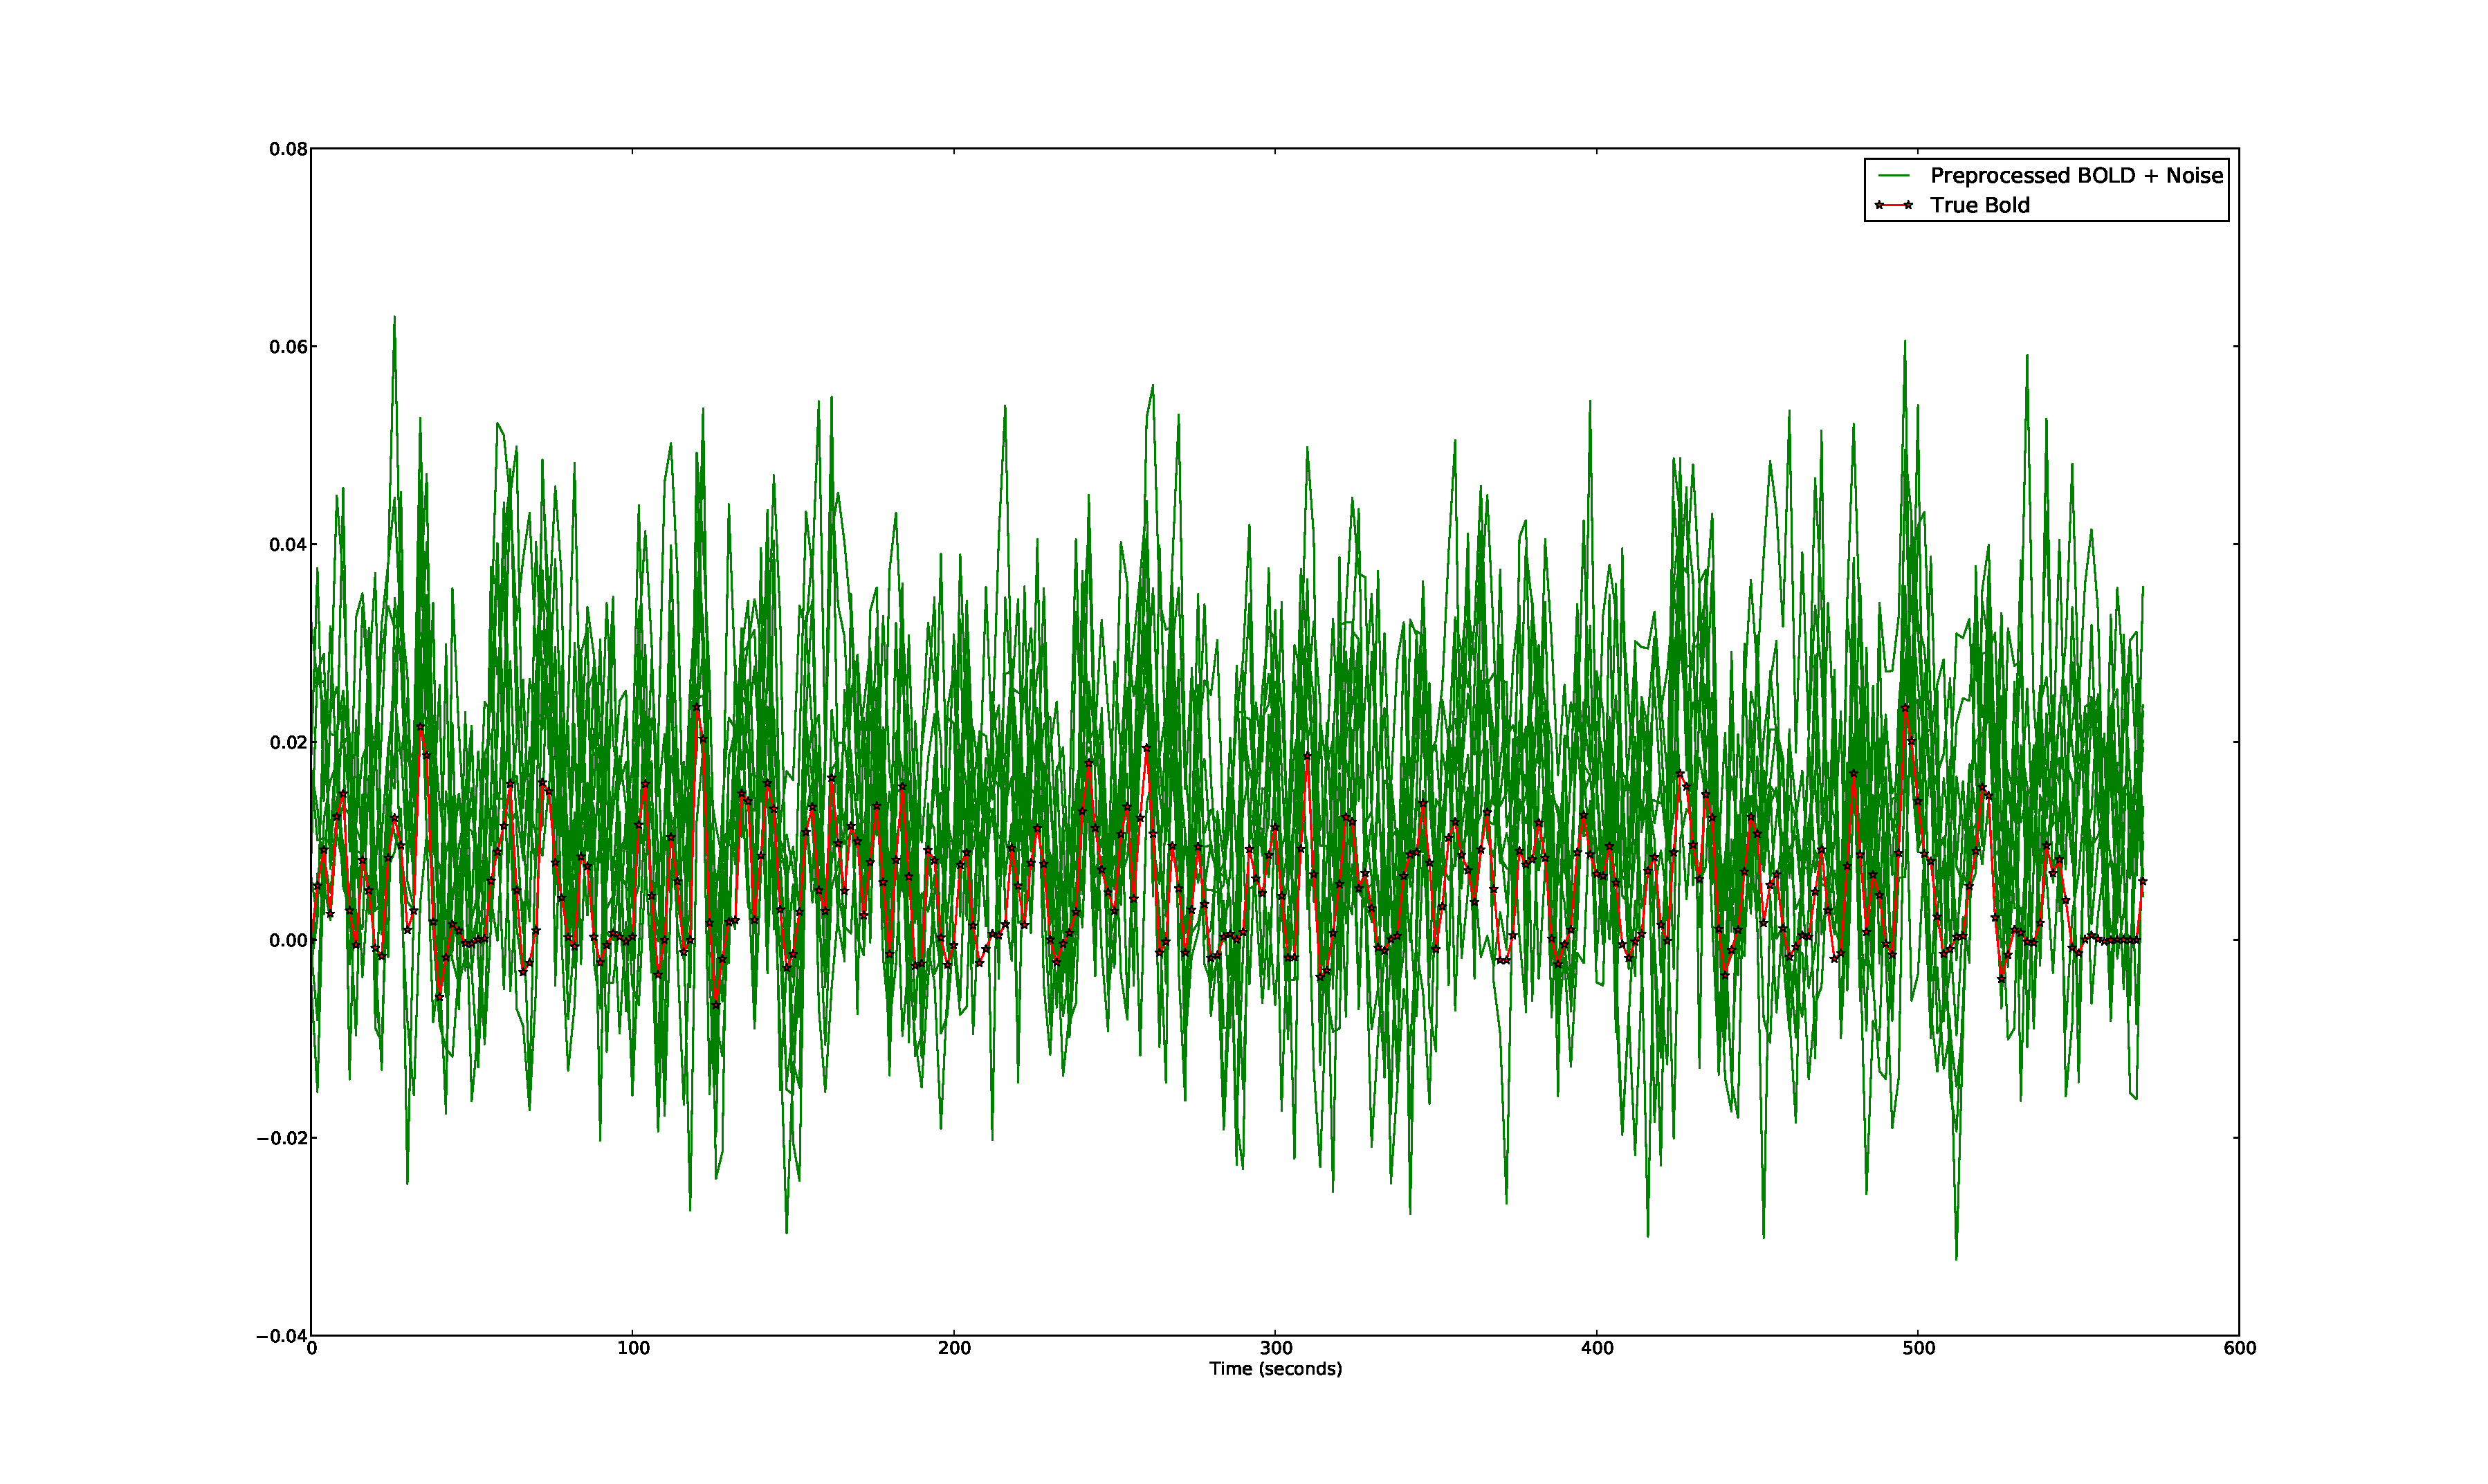
\includegraphics[clip=true,trim=6cm 2cm 6cm 3.5cm,width=7cm]{images/preprocessed_highnoise}
\caption{A comparison of the preprocessed signals for the high noise case.}
\label{fig:PreprocessedHighNoise}
\end{figure}
\begin{figure}
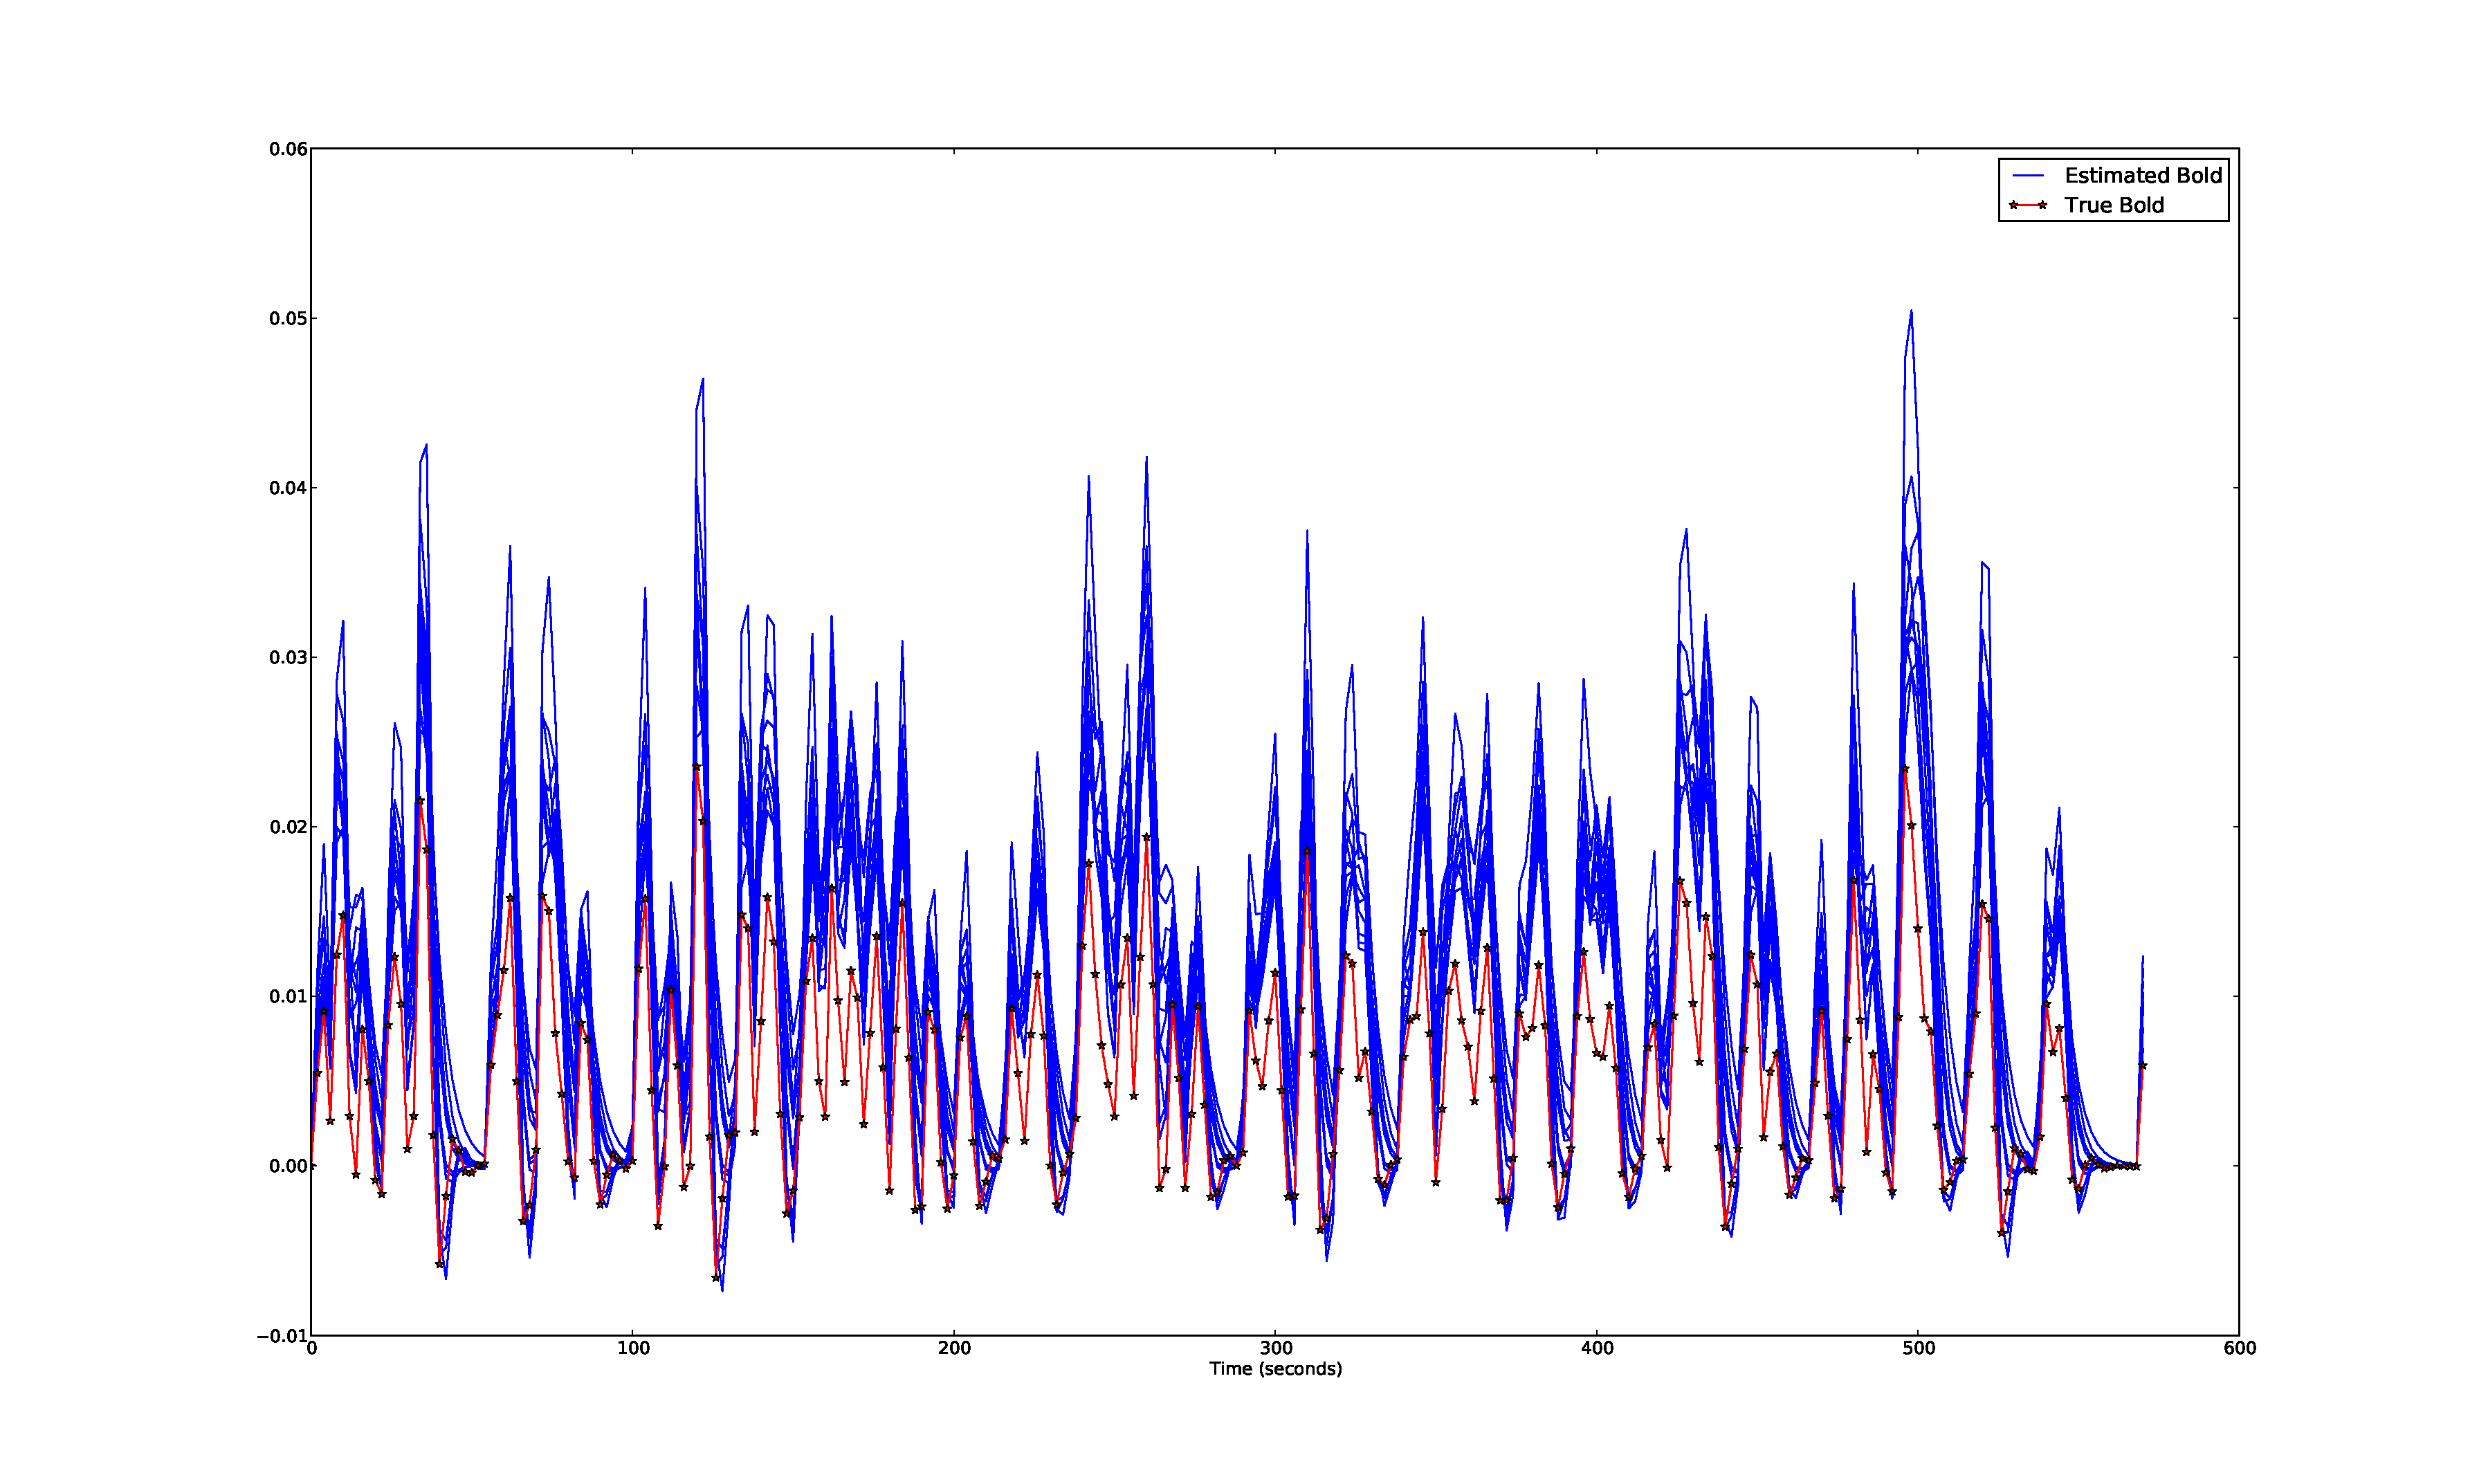
\includegraphics[clip=true,trim=6cm 2cm 6cm 3.5cm,width=17cm]{images/comparison_highnoise}
\caption{A comparison of the fitted signals for the high noise case.}
\label{fig:FitComparisonHighNoise}
\end{figure}
\begin{figure}
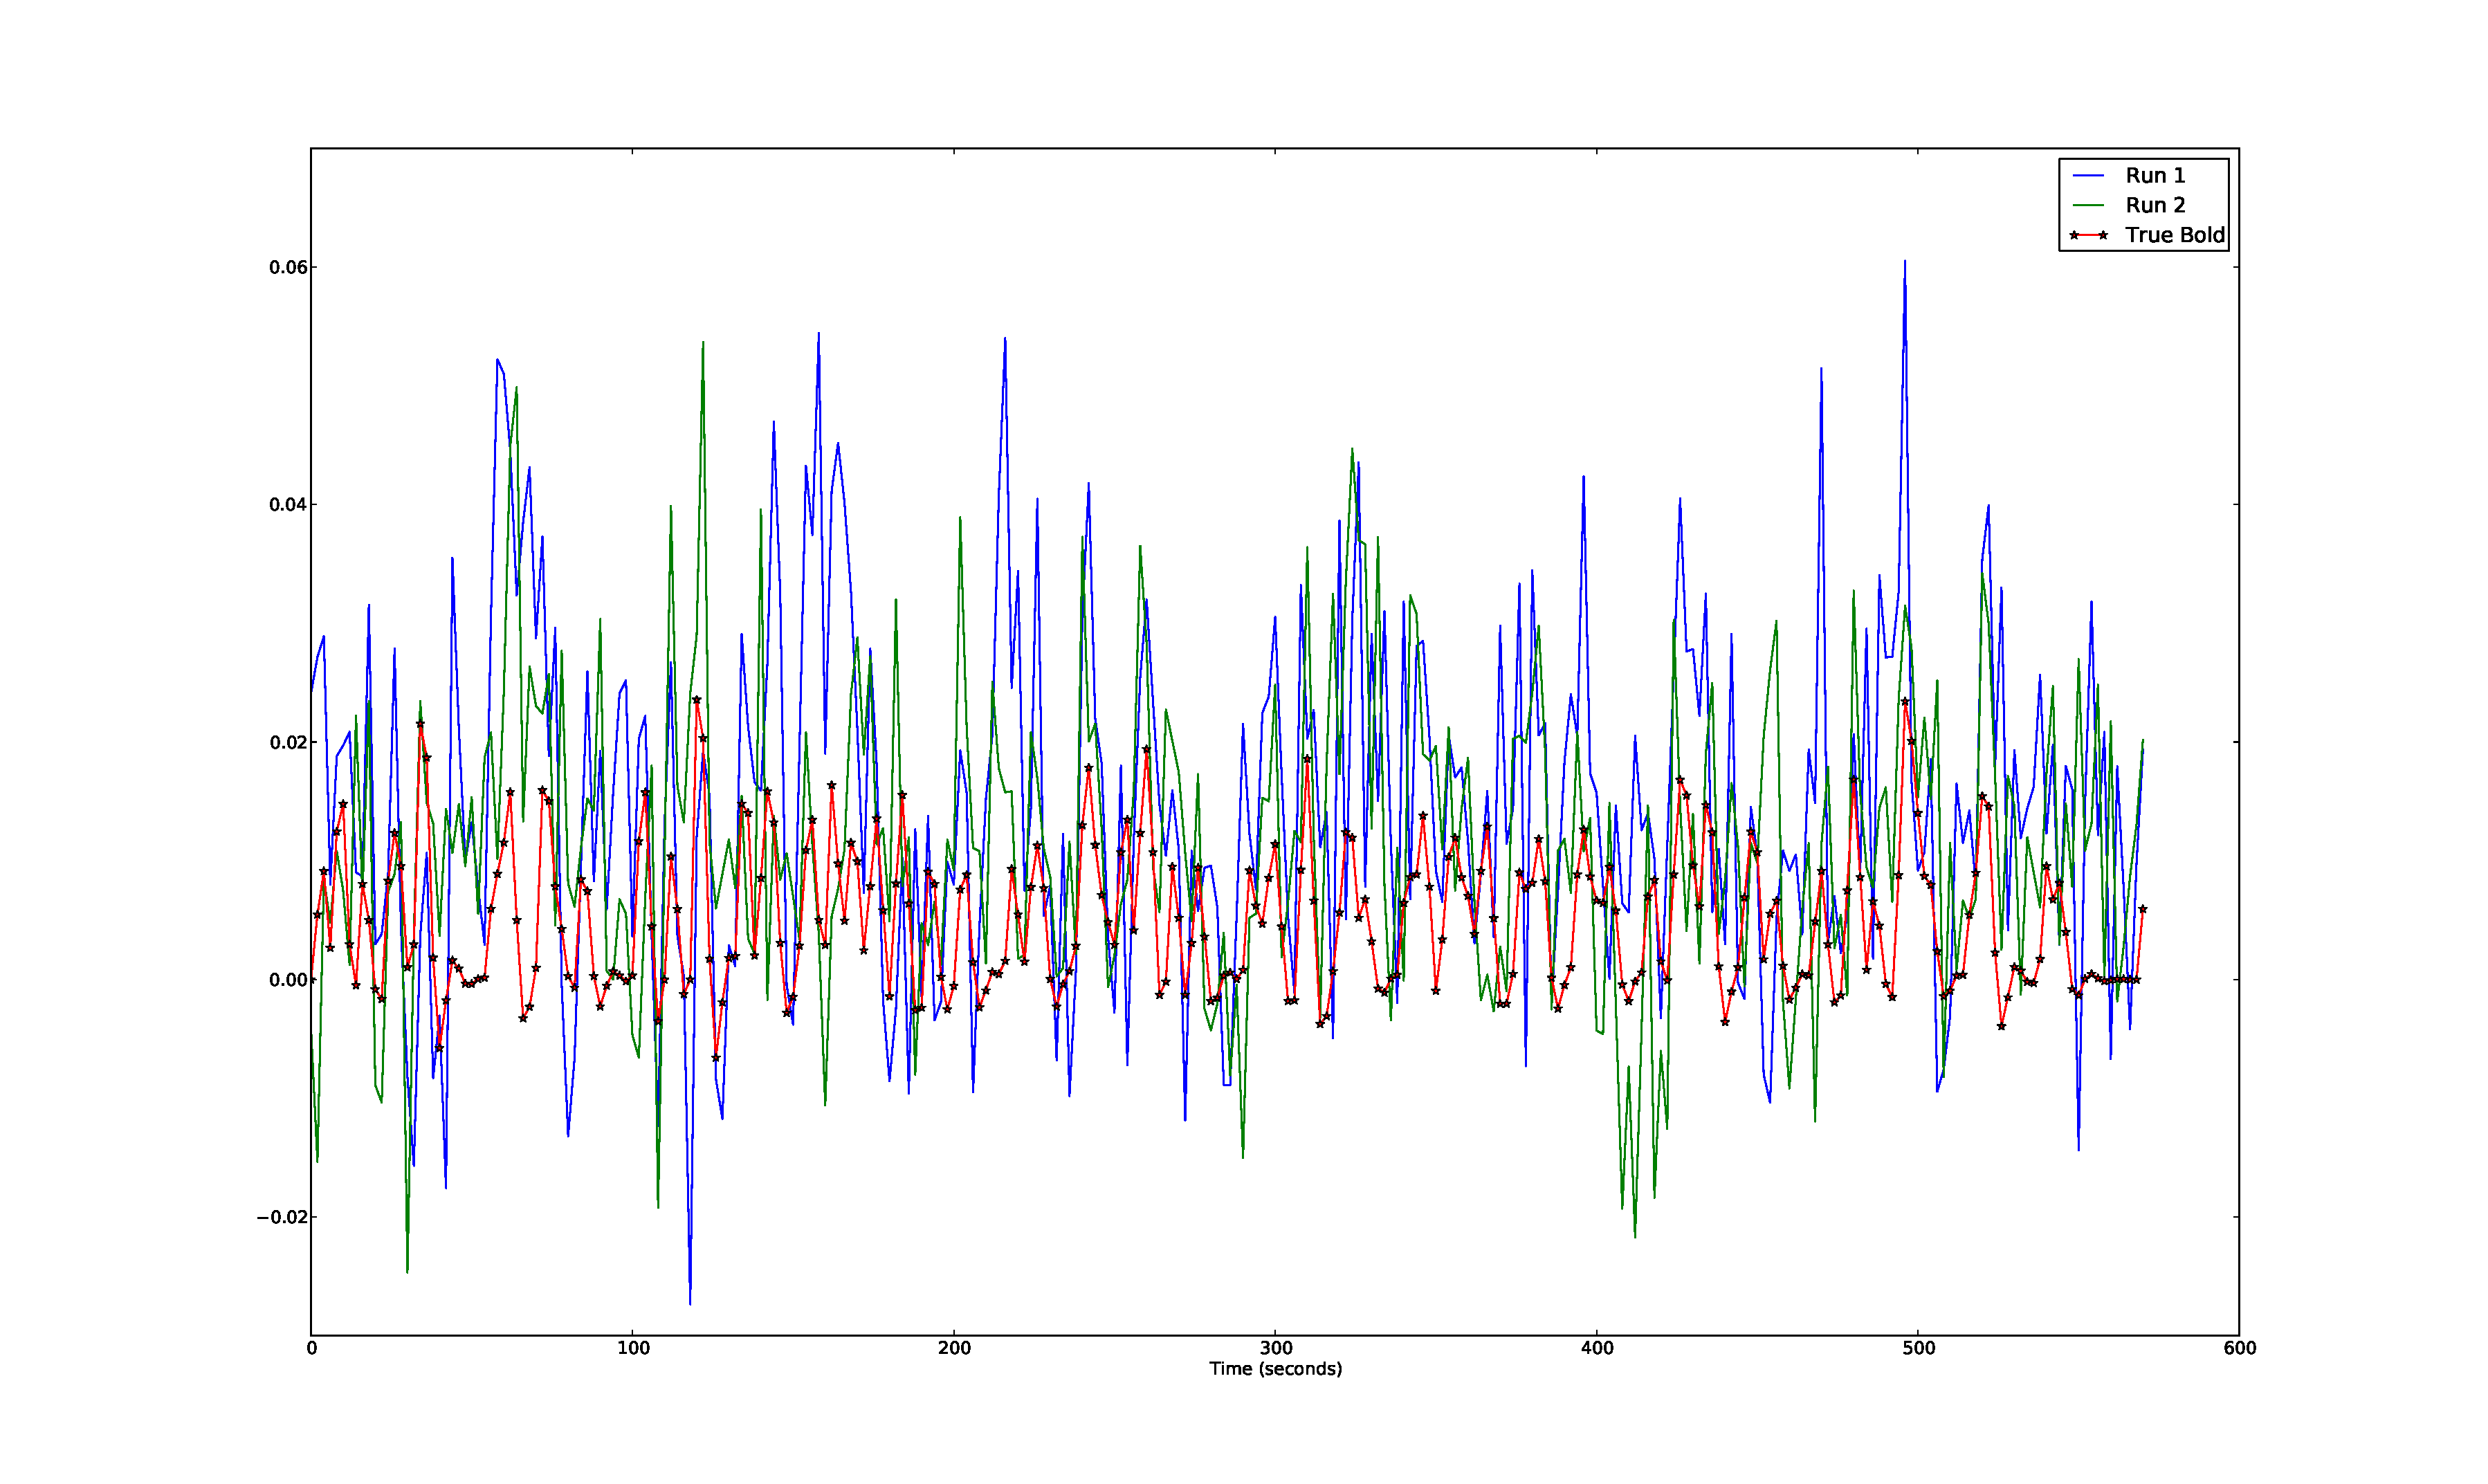
\includegraphics[clip=true,trim=6cm 2cm 6cm 3.5cm,width=17cm]{images/highnoise_56_noise}
\caption{Two particular preprocessed noise realizations for the high noise case.}
\label{fig:NoiseComparisonJustTwo}
\end{figure}

\begin{figure}
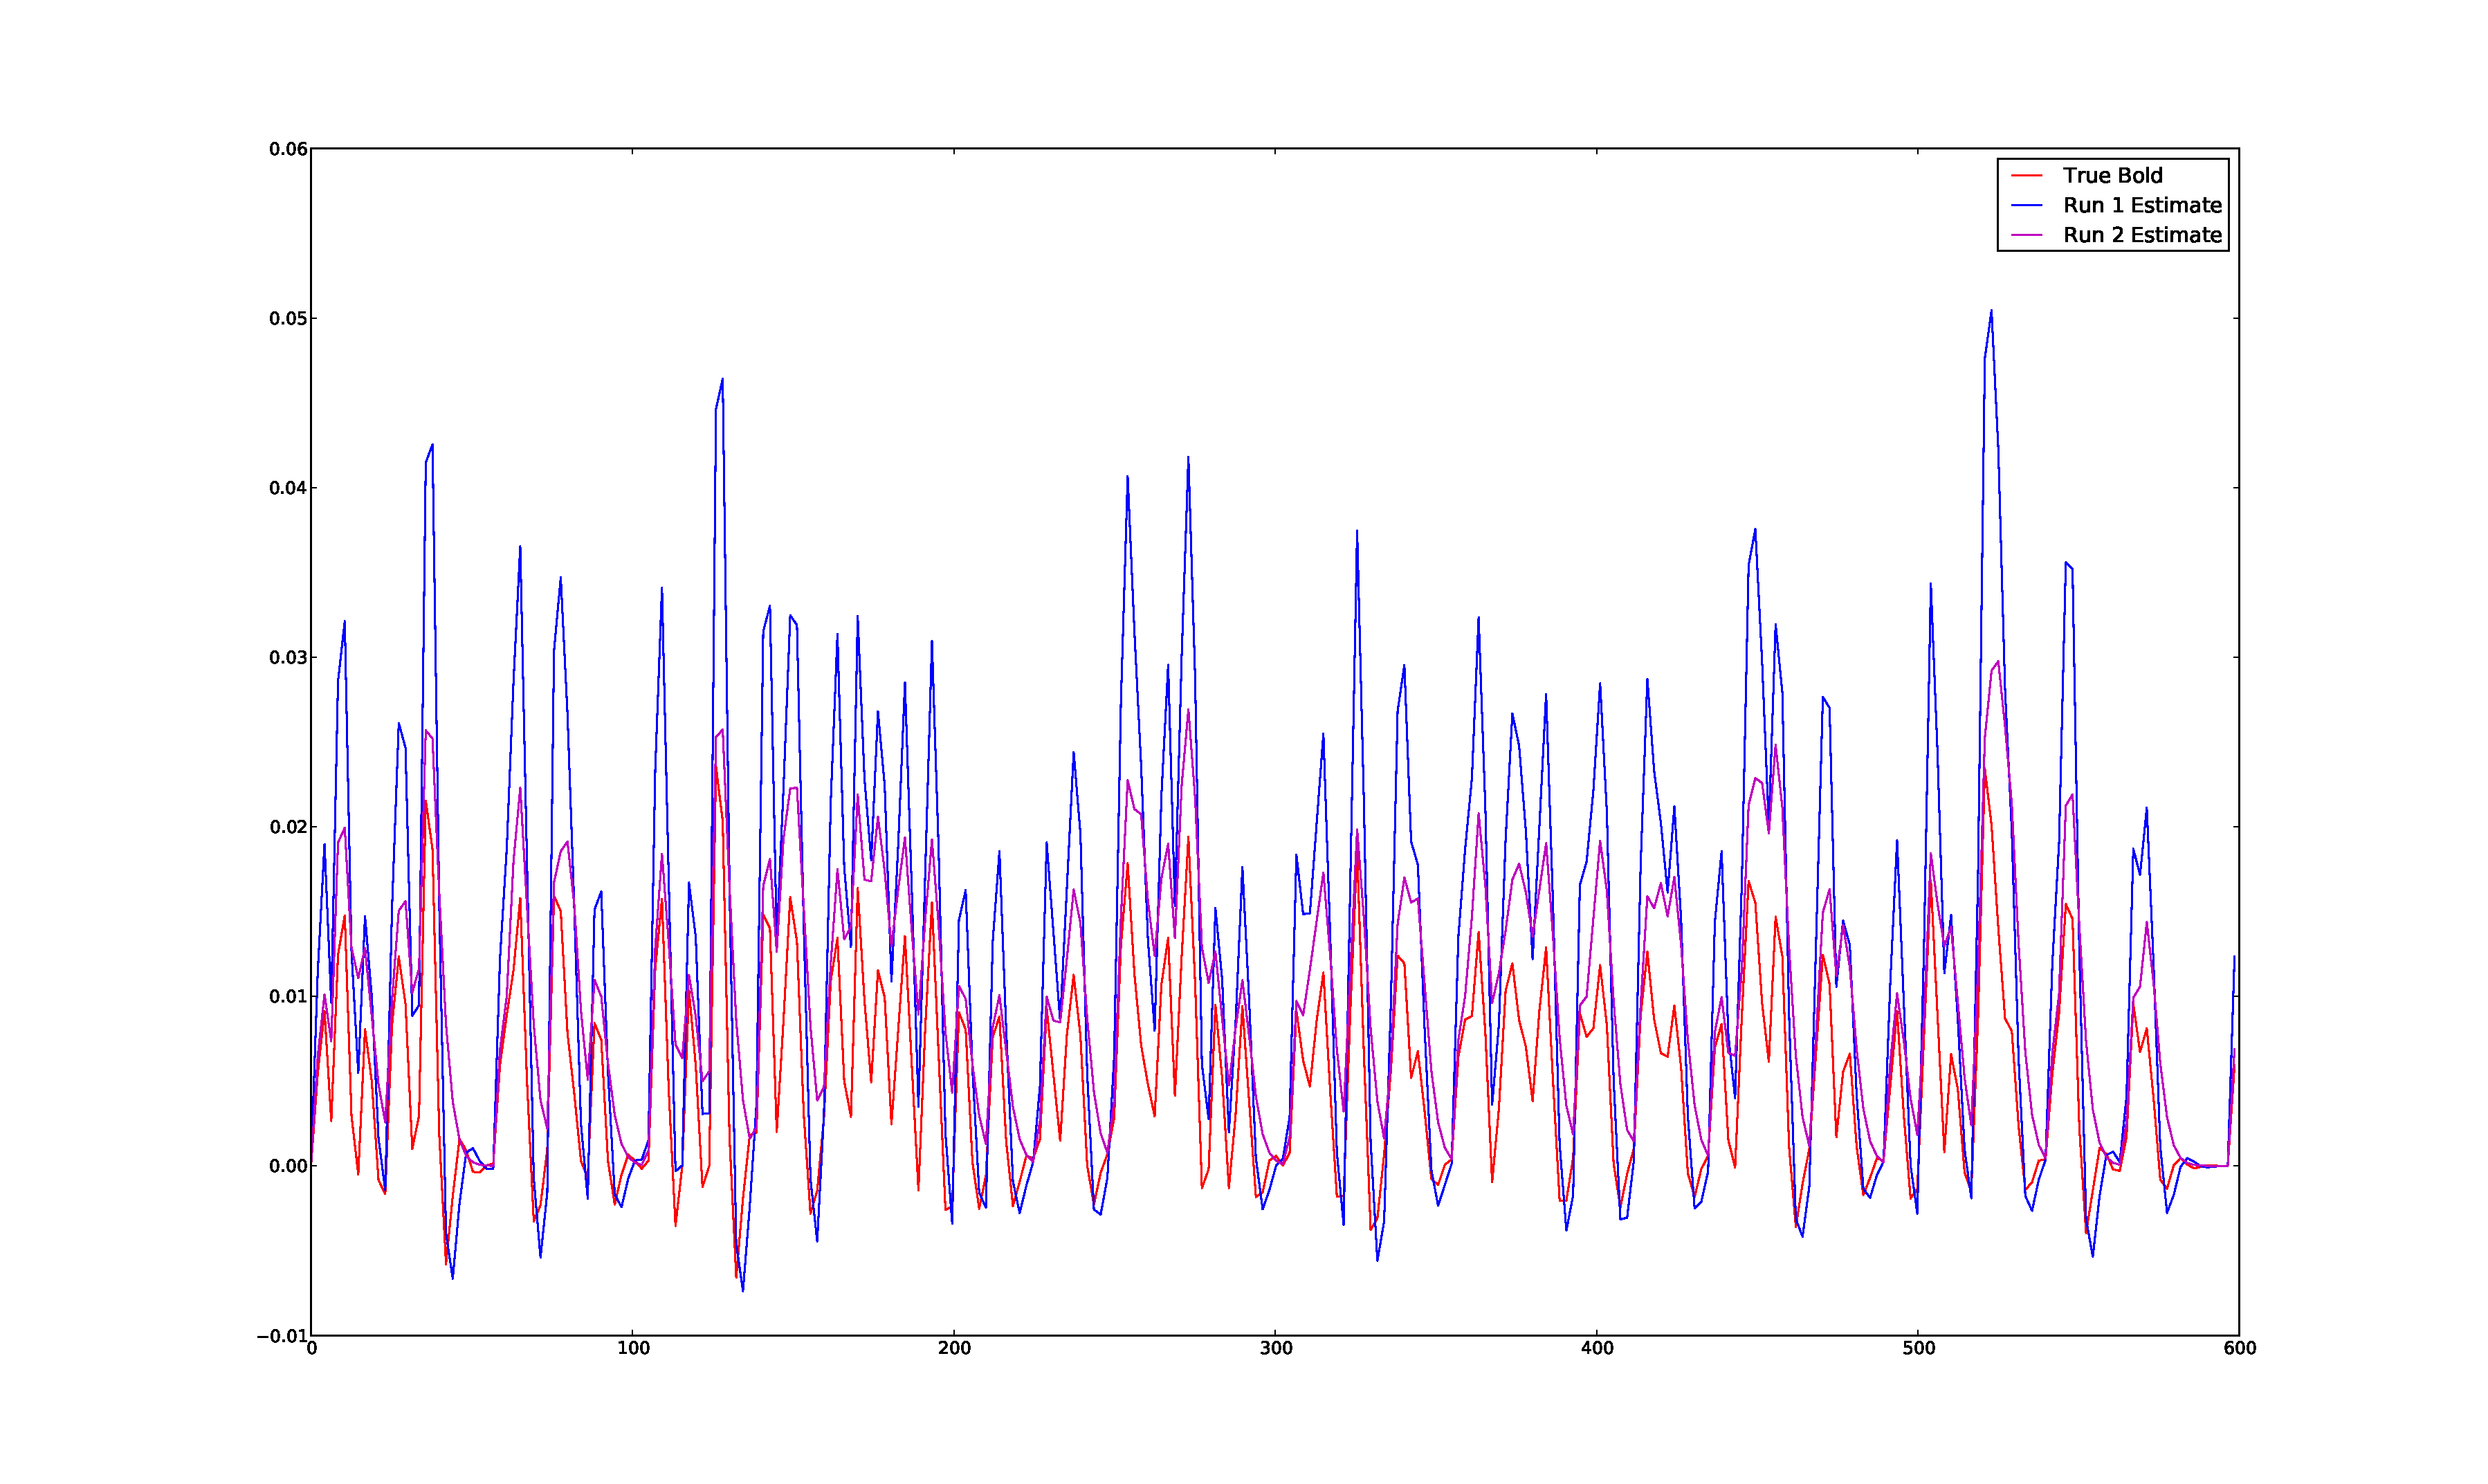
\includegraphics[clip=true,trim=6cm 2cm 6cm 3.5cm,width=17cm]{images/comparison_highnoise_just2}
\caption{The results for the noise realizations shown in \autoref{fig:NoiseComparisonJustTwo}.}
\label{fig:FitComparisonHighNoiseJust2}
\end{figure}

For the high noise simulation, the exact same procedure was performed as with the lower
noise simulation except that $\sigma_y$ and $\sigma_x$ were set to $.01$ and $.005$,
respectively. This is an order of magnitude higher than the previous tests, and indeed the
noise appears to dominate the output, as seen in \autoref{fig:HighNoiseRealization}.  
As before, the results of preprocessing are helpful in identifying the reason for
bias in the estimated output signal; thus the preprocessed signals are shown in 
\autoref{fig:PreprocessedHighNoise}. The results of the particle filter
for each of the eleven runs are shown in \autoref{fig:FitComparisonHighNoise}. 
As before, the preprocessing led the algorithm
to somewhat higher activation levels, and it would appear that the subtleties of
different time constants are being lost due to the noise. This is easily seen
by observing the post stimulus undershoots; many of the estimated time series
have no post-stimulus undershoot but rather decay directly to the base level.

\begin{table}[t]
\centering
\begin{tabular}{|c | c | c | c | c | c | c | c | c | c |}
\hline 
$\tau_0$ & $\alpha$ & $E_0$    & $V_0$    & $\tau_s$ & $\tau_f$ & $\epsilon$  & $ \sum \tau $ & $\sqrt{MSR}$  & $\sqrt{MSE}$\\
\hline 
\rowcolor[gray]{.8}
1.45 & .3 & .47 & .044 & 1.94 & 1.99 & 1.8  & 5.38 &  & \\
\hline 
\hline 
1.1900 & 0.2349 & 0.4223 & 0.128  & 1.0147 & 2.4779 & 1.1168 & 4.6826 &0.01406 &0.01573   \\
0.9721 & 0.2190 & 0.3051 & 0.061  & 0.5780 & 1.9960 & 3.4613 & 3.5461 &0.01373 &0.01378   \\
1.5795 & 0.1415 & 0.3380 & 0.1089 & 0.5843 & 2.1247 & 1.7834 & 4.2885 &0.01275 &0.01577   \\
1.1094 & 0.2374 & 0.5349 & 0.0351 & 1.2186 & 3.0736 & 2.3504 & 5.4016 &0.01673 &0.01154    \\
1.1071 & 0.2753 & 0.3365 & 0.0316 & 1.5057 & 2.6518 & 4.1910 & 5.2646 &0.01370 &0.01222   \\
0.5803 & 0.4793 & 0.4135 & 0.1189 & 0.9756 & 3.6902 & 1.0008 & 5.2461 &0.01150 &0.01316   \\
\rowcolor[rgb]{.9,.5,.5}
1.2952 & 0.2596 & 0.2756 & 0.2595 & 1.7026 & 2.8458 & 0.6617 & 5.8436 &0.01555 &0.01790   \\
\rowcolor[rgb]{.5,.5,.9}
1.5185 & 0.2199 & 0.2835 & 0.0742 & 0.8882 & 3.0771 & 1.7393 & 5.4838 &0.01205 &0.01246   \\
0.6874 & 0.3283 & 0.3979 & 0.1561 & 1.0778 & 3.1158 & 0.6643 & 4.8810 &0.01510 &0.01258   \\
1.0170 & 0.285  & 0.3474 & 0.0567 & 1.5877 & 2.6516 & 2.2852 & 5.2563 &0.01249 &0.01343   \\
0.9925 & 0.298  & 0.3221 & 0.2094 & 0.4276 & 2.2108 & 1.0167 & 3.6308 &0.01217 &0.01506   \\
\hline                                                                          
1.0954 & 0.2708 & 0.3615 & 0.1126 & 1.0510 & 2.7196 & 1.8428 & 4.8659 &0.01362 &0.01397\\
\hline 
\end{tabular}
\caption{Estimated Parameters on 10 different runs with high noise. First row is the true parameters.
The red row is Run 1 and the blue row is Run 2, as named in  \autoref{fig:NoiseComparisonJustTwo}
and \autoref{fig:FitComparisonHighNoiseJust2}}
\label{tab:HighNoiseResults} 
\end{table}

It is interesting to consider how the preprocessing and noise may effect the
parameters of the fitting model. Consider two runs, shown in 
\autoref{fig:NoiseComparisonJustTwo}, out of the previous eleven. 
Run 1 has higher peaks, in spite of the fact that both signals are based
on the same underlying signal. There also appears
to be more drift than the 20 measurements per knot could fit, which explains run 1's
prolonged increase at 170 seconds in. Interestingly, run 1 and run 2 have different
aspects of the signal that match better. Run 2 had a much better match to the 
peaks, when compared to the true signal, yet run 1 matched the post-stimulus
undershoot better. Its worth noting however, that the post-stimulus undershoots
here are much shorted than the observed prolonged post-stimulus undershoot
discussed in \autoref{sec:Post Stimulus Undershoot}. 
Despite the rather significant amount of noise, the ultimate results are 
actually rather good. \autoref{tab:HighNoiseResults} shows
the square-root mean-squared-error for all eleven runs, and highlights the two runs analyzed 
in \autoref{fig:ConvergenceRuns1} and \autoref{fig:ConvergenceRuns2}.

\begin{figure}
\subfigure[$\tau_0$, $\alpha$, $E_0$, $V_0$, Run 1]
{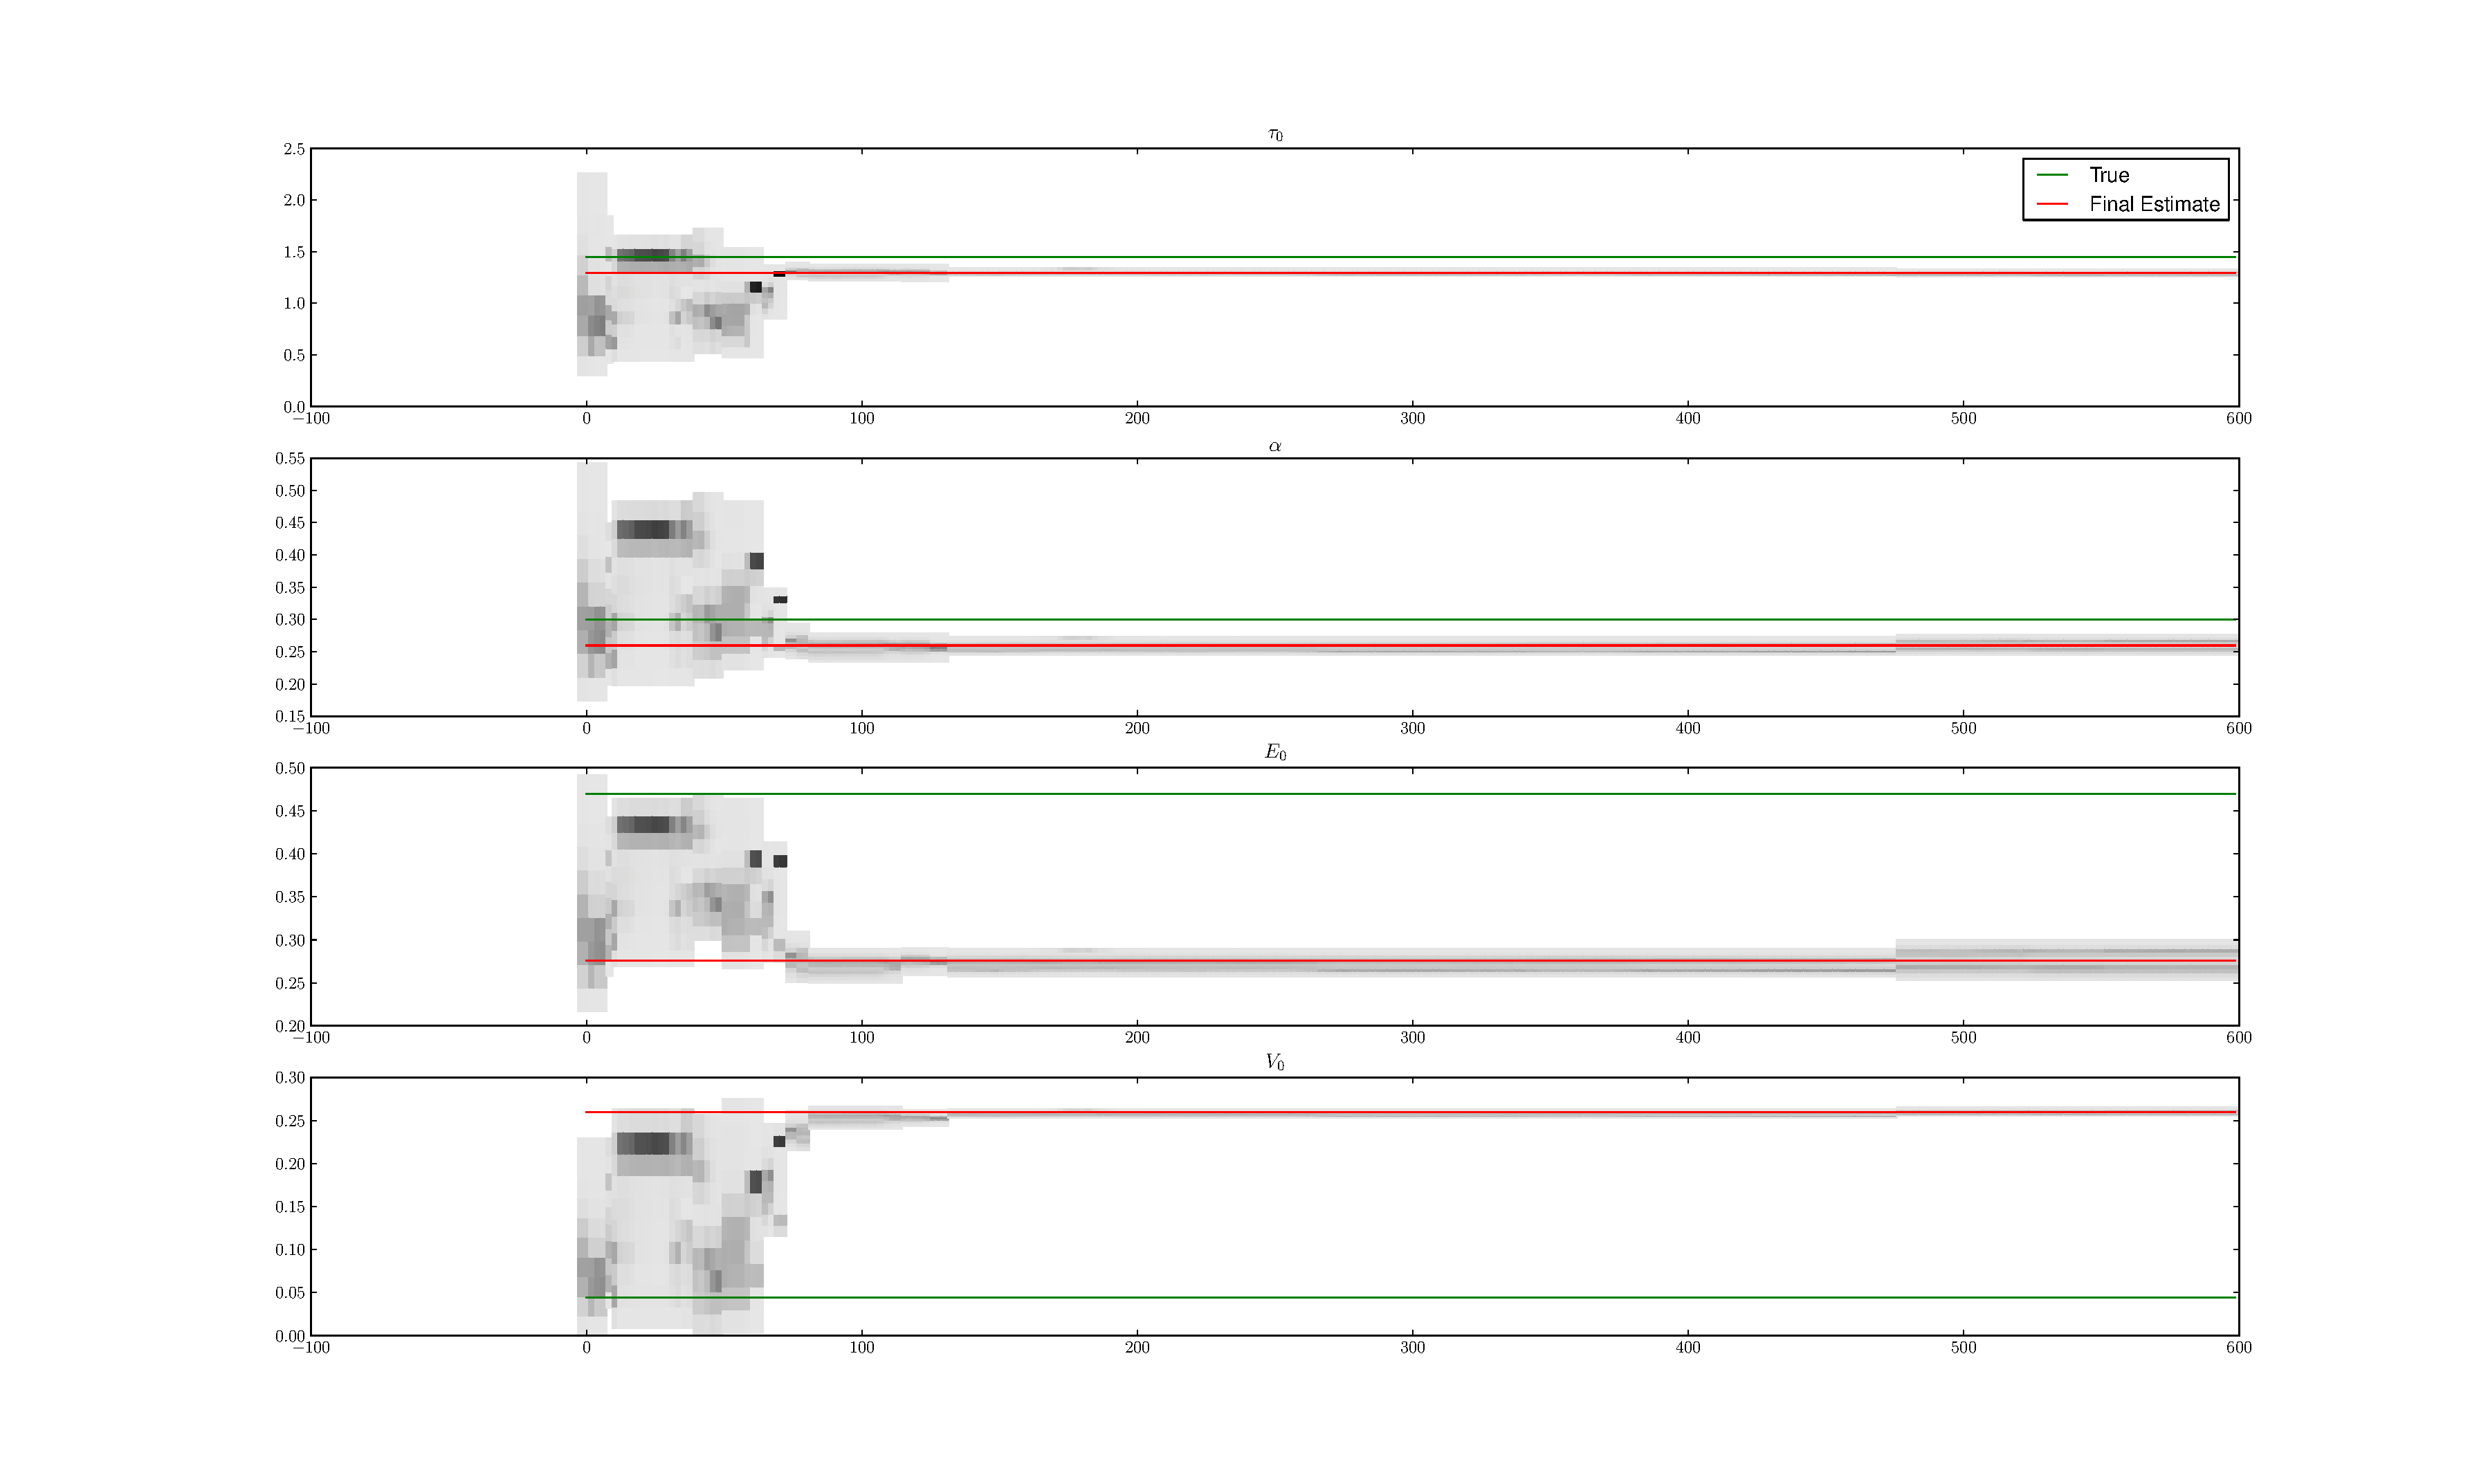
\includegraphics[clip=true,trim=6cm 2cm 6cm 3cm, width=14cm]{images/highnoise_run5_1}}\\
\end{figure}
\begin{figure}
\subfigure[$\tau_s$, $\tau_f$, $\epsilon$, $V$, Run 1] 
{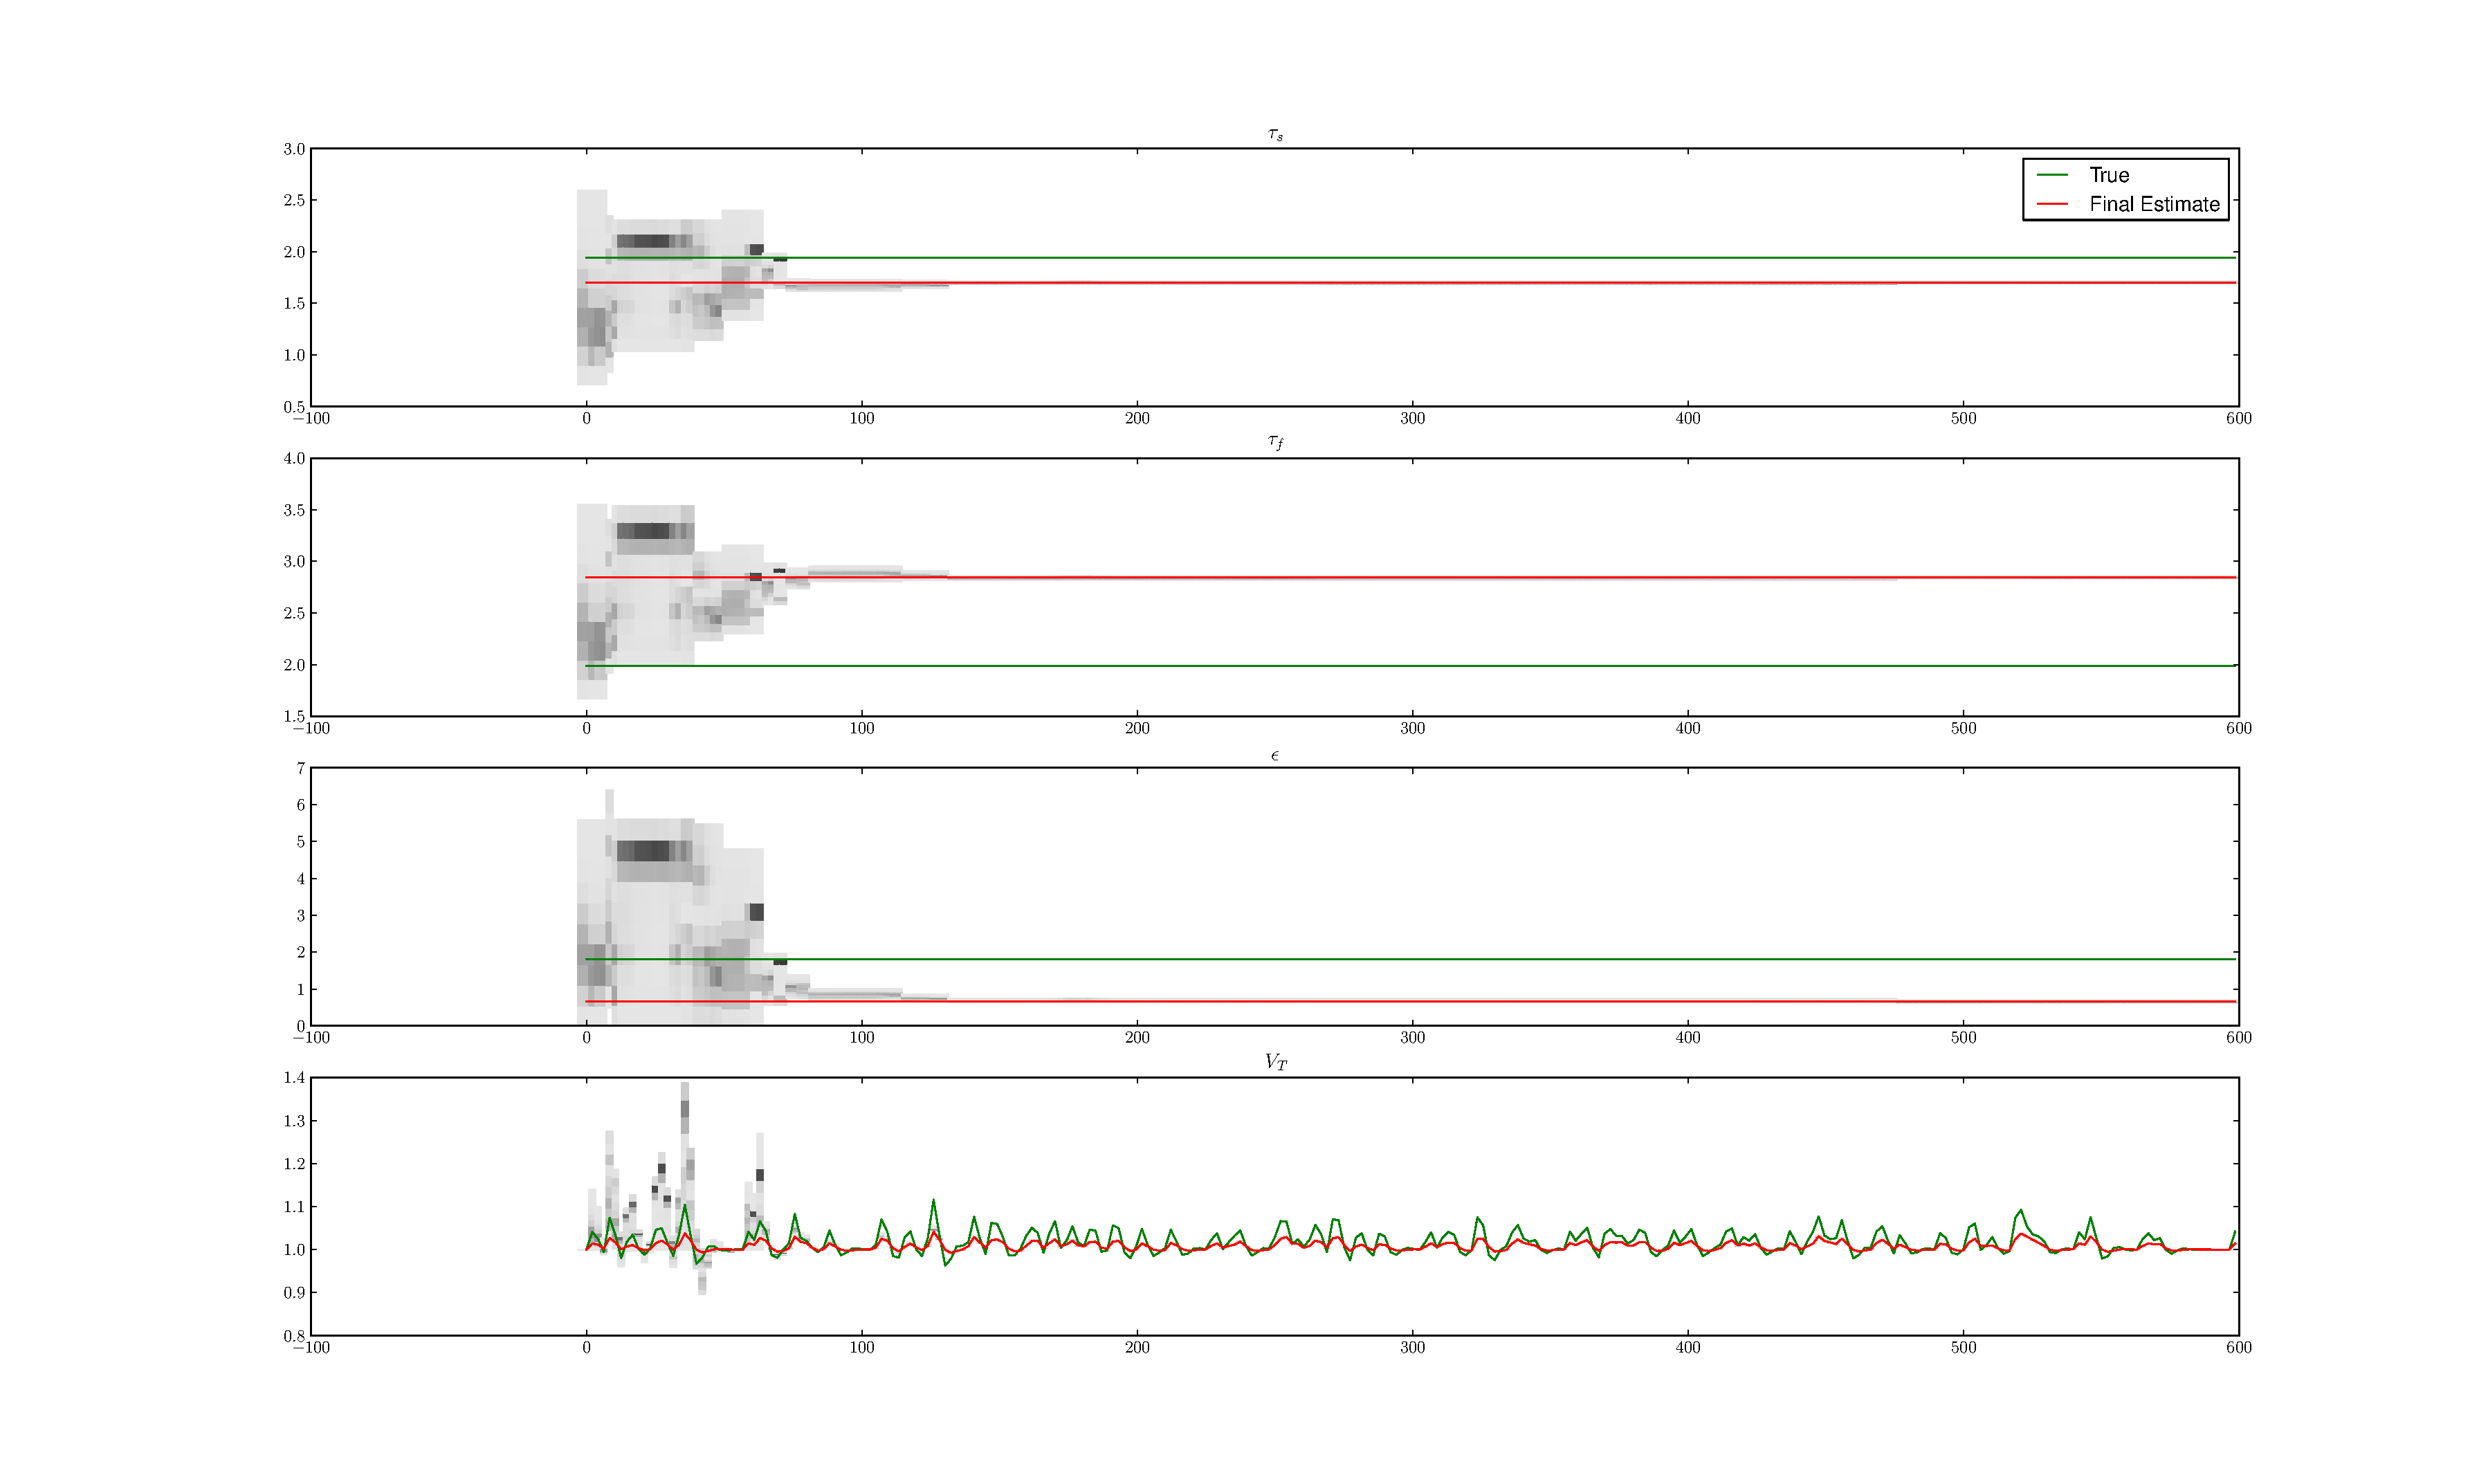
\includegraphics[clip=true,trim=6cm 2cm 6cm 3cm, width=14cm]{images/highnoise_run5_2}}\\
\end{figure}
\begin{figure}
\subfigure[$Q$, $S$, $F$, $BOLD$, Run 1 ]
{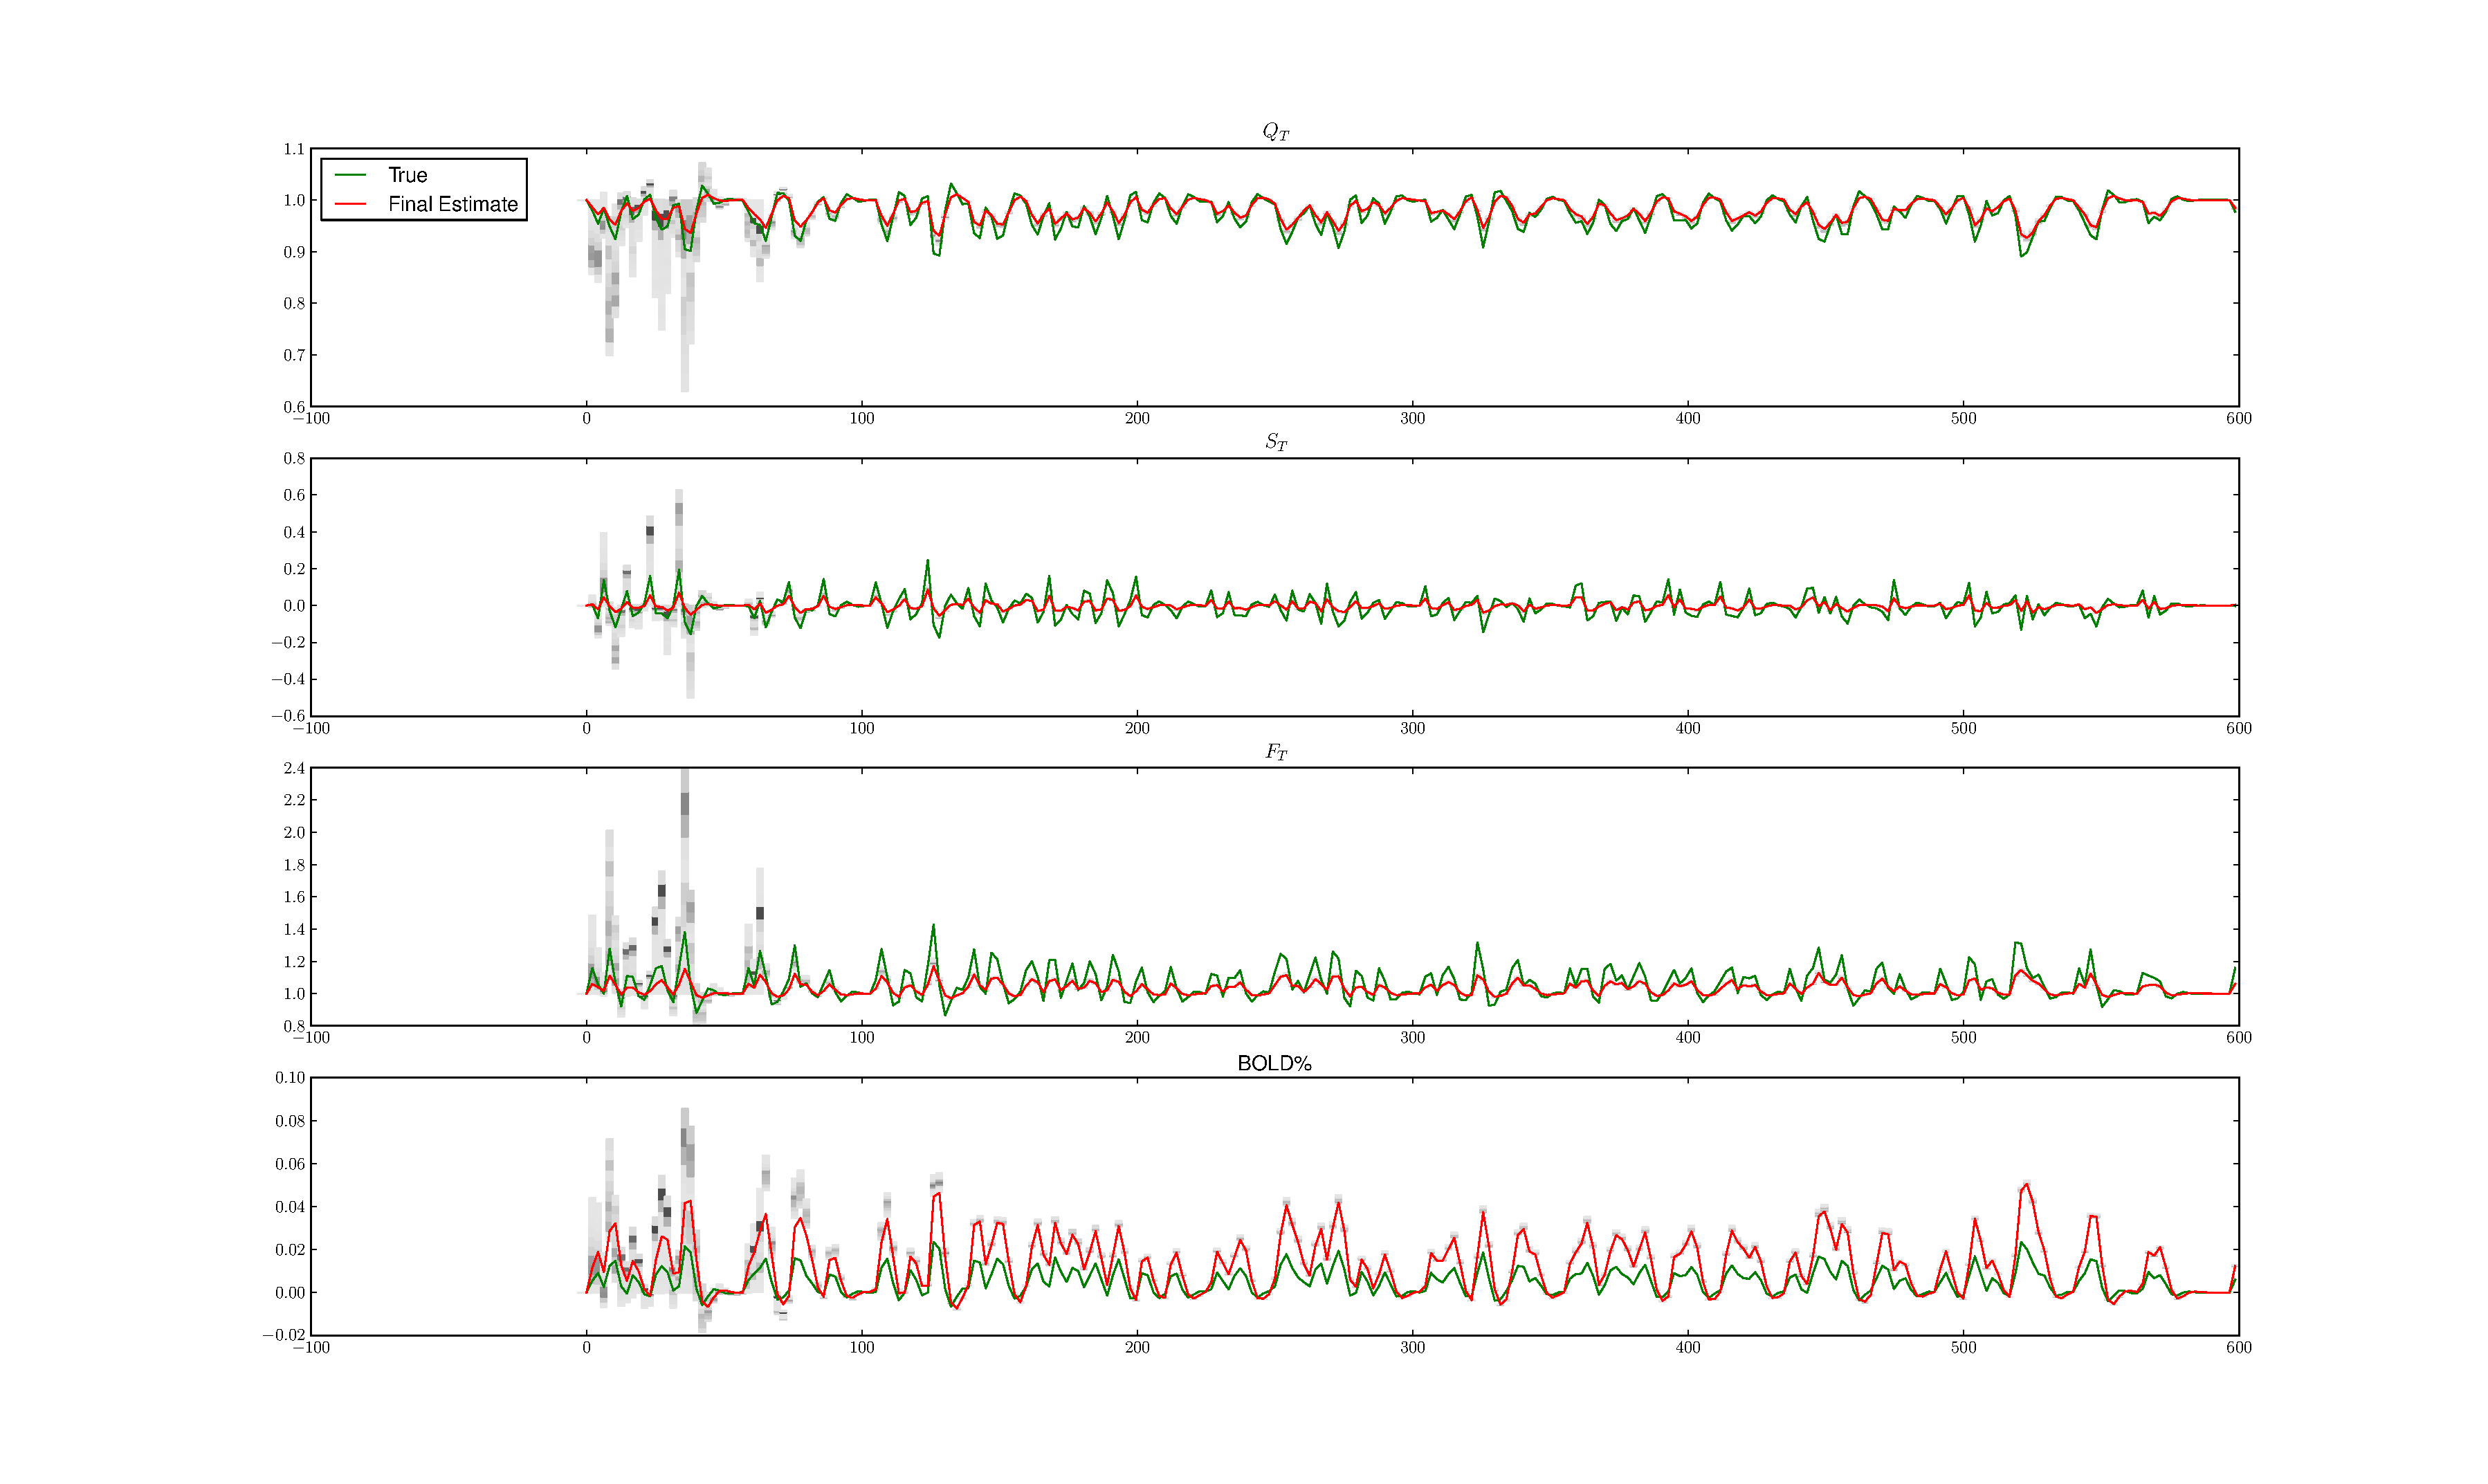
\includegraphics[clip=true,trim=6cm 2cm 6cm 3cm, width=14cm]{images/highnoise_run5_3}}
\caption{Converging histogram for parameters during run 1, as in \autoref{fig:NoiseComparisonJustTwo}.}
\label{fig:ConvergenceRuns1}
\end{figure}

\begin{figure}
\subfigure[$\tau_0$, $\alpha$, $E_0$, $V_0$, Run 2]
{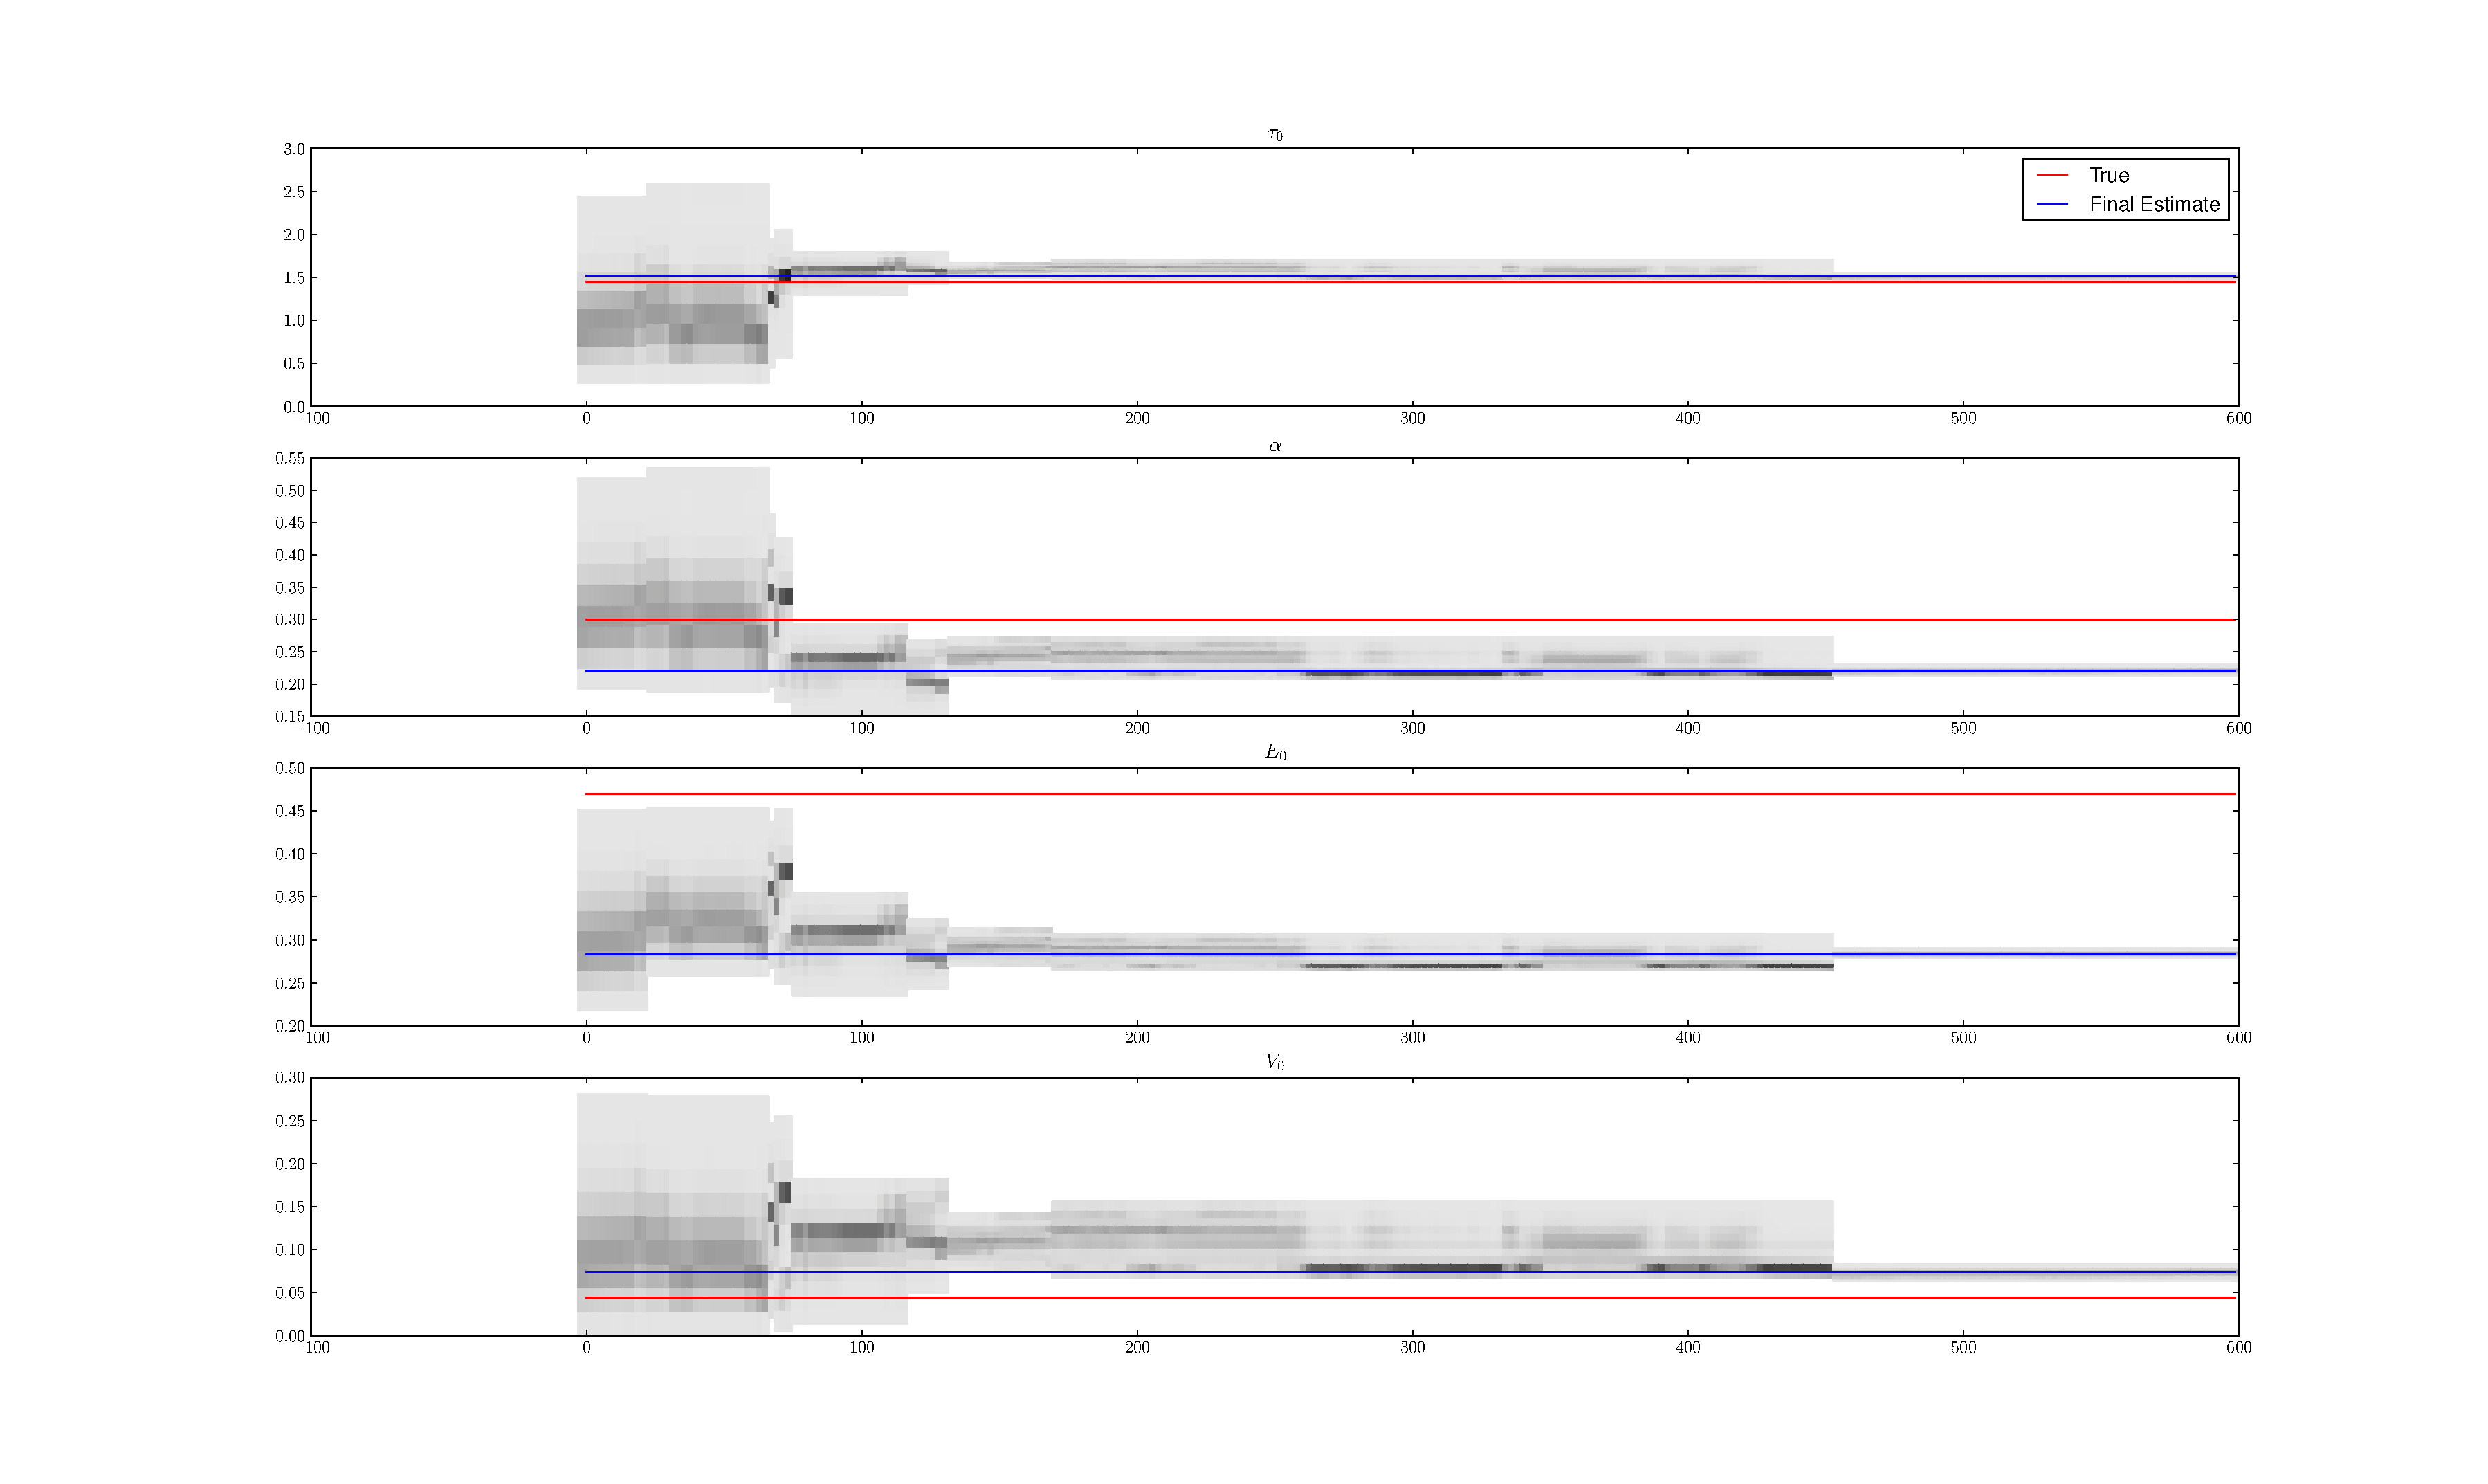
\includegraphics[clip=true,trim=6cm 2cm 6cm 3cm, width=14cm]{images/highnoise_run6_1}}\\
\end{figure}
\begin{figure}
\subfigure[$\tau_s$, $\tau_f$, $\epsilon$, $V$, Run 2] 
{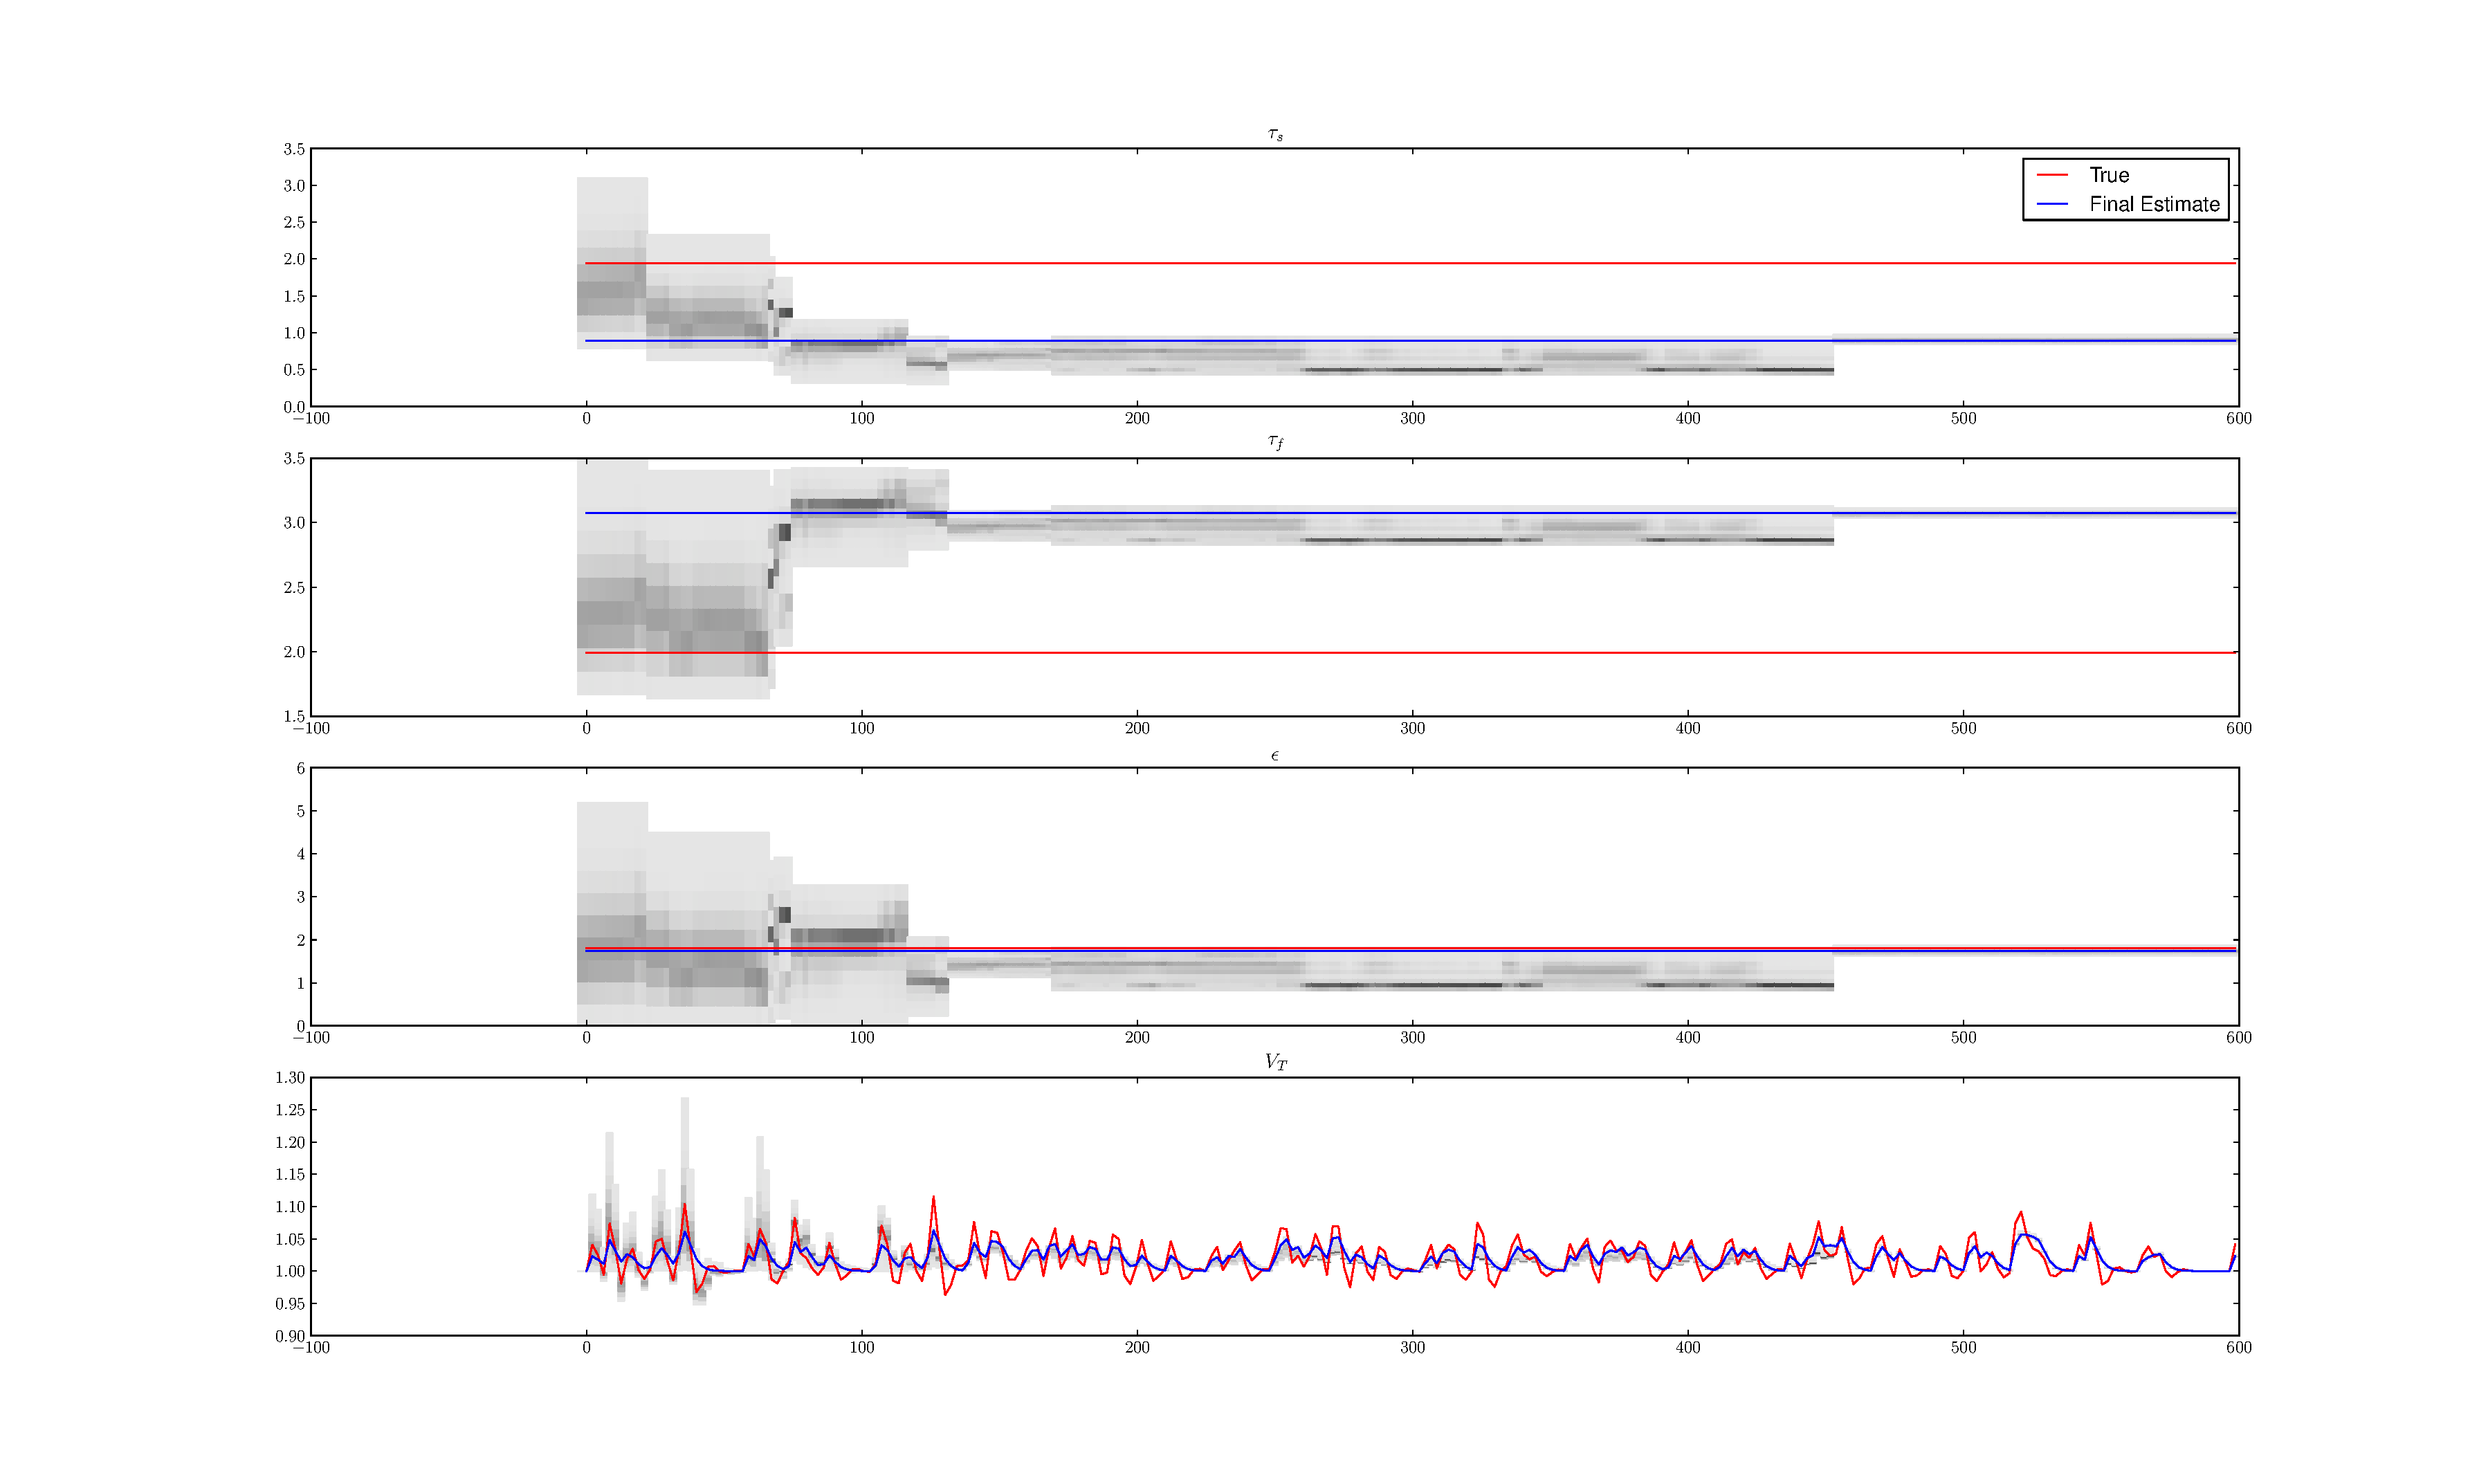
\includegraphics[clip=true,trim=6cm 2cm 6cm 3cm, width=14cm]{images/highnoise_run6_2}}\\
\end{figure}
\begin{figure}
\subfigure[$Q$, $S$, $F$, $BOLD$, Run 2 ]
{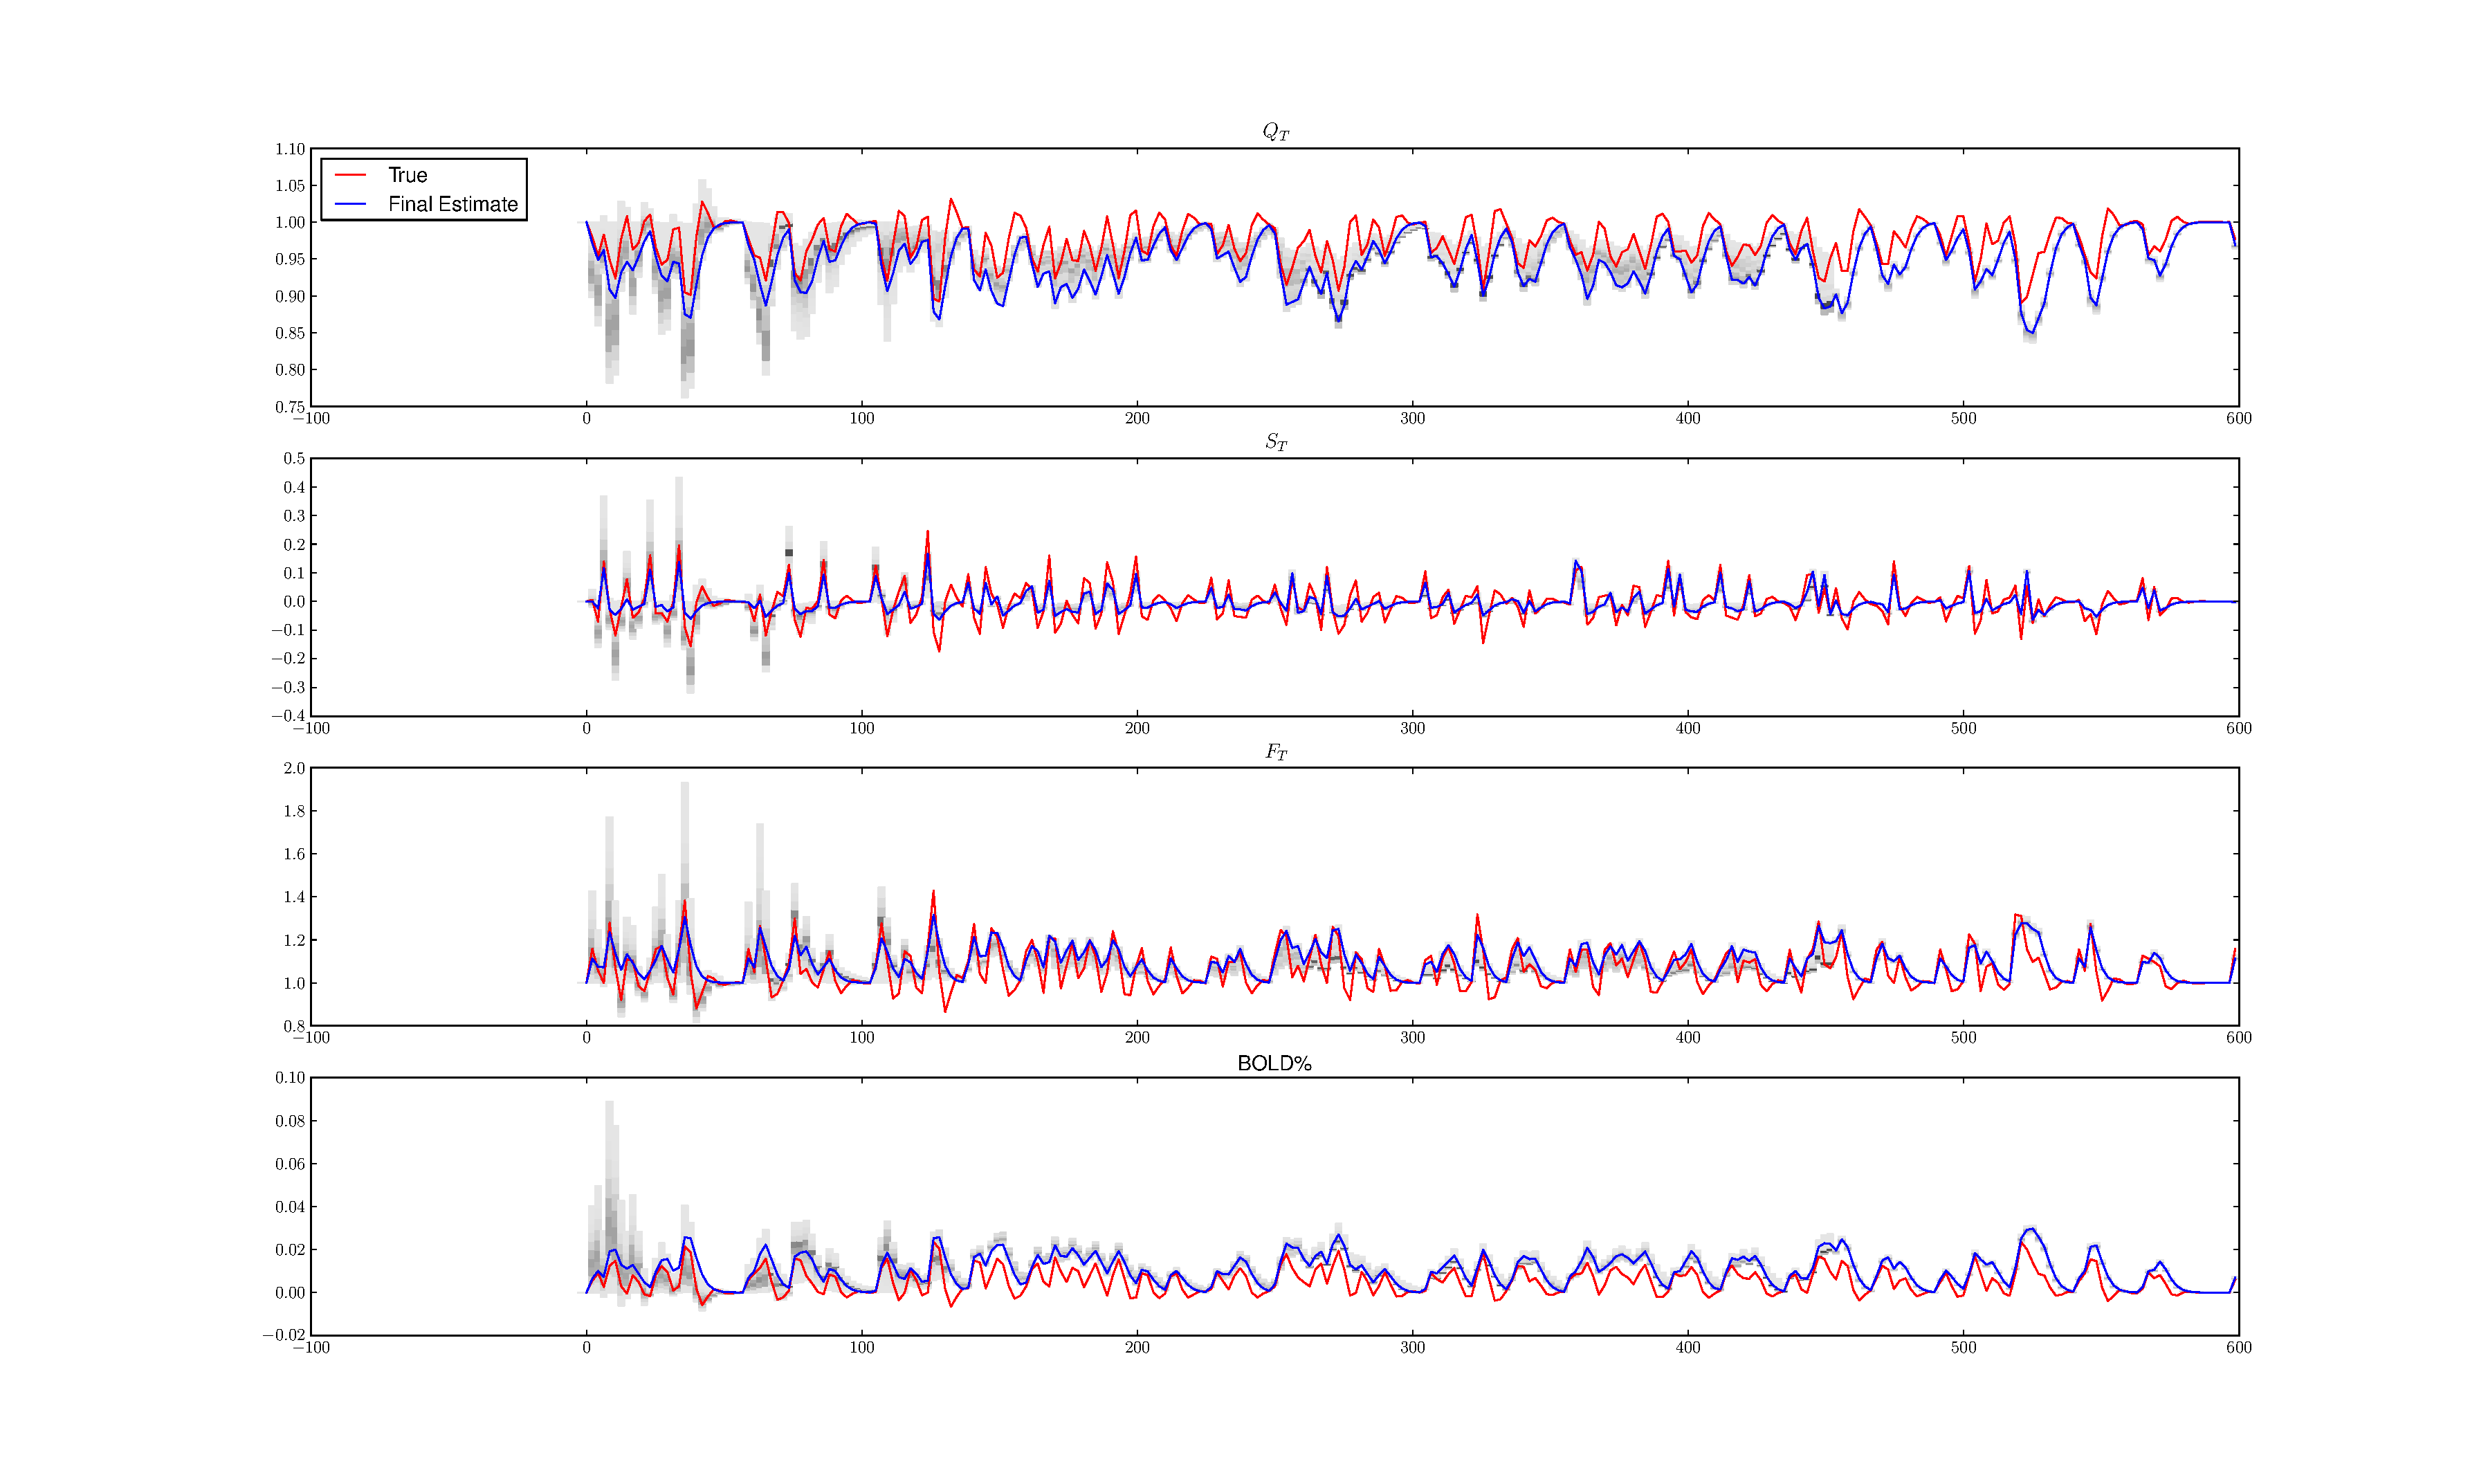
\includegraphics[clip=true,trim=6cm 2cm 6cm 3cm, width=14cm]{images/highnoise_run6_3}}
\caption{Converging histogram for parameters during run 2, as in \autoref{fig:NoiseComparisonJustTwo}.}
\label{fig:ConvergenceRuns2}
\end{figure}

There are a number of interesting convergence properties of the
particle filter when more noise is present, as both \autoref{fig:ConvergenceRuns1} and
\autoref{fig:ConvergenceRuns2} show. The particle filter seems to converge
significantly faster; as points tend to be further out on the weighting function. This
also causes significantly more resampling which is the explanation for the percieved
jumps in resolution that occur from time to time. Here it is clear that the mode and
the mean will not be substantially different. Because of the increased noise, its likely
that the weighting function is not sufficiently wide to account for the measurement noise.

The parameters arrived at for all ten filter runs are shown in \autoref{tab:HighNoiseResults}.
Clearly the additional noise have resulted in much more sporadic results. This is often the 
result when the particle filter converges too fast, a result of the weighting functions' variance
being smaller than the measurement noise ($.005$ vs. $.01$). The error
certainly suffers due to this effect.

%NO SIGNAL, LOW NOISE
\subsection{Pure-Noise, low magnitude}
\label{sec:PureNoiseLowMag}
The two final single-voxel tests force the particle filter to attempt to learn a noise-only
time series. In the first test the noise used will be the same as that from the \autoref{sec:HighNoise},
$\sigma_x = .01, \sigma_y = .005$. The parameters will be set the same as well, but the
stimulus/input neuronal efficiency ($\epsilon$) will be set to 0. In effect it is a region of the brain for
which no visual stimulus induces activity. The question then is how the
particle filter will respond to signal that does not correlate with the input, and how
the output may be differentiated from a time series that does. The time series'
are shown in \autoref{fig:NoiseOnly}, the preprocessed versions are shown in \autoref{fig:PreprocessedNoiseOnly}.
The line fits are shown in \autoref{fig:fits_noiseonly}. 

\begin{figure}[H]
\centering
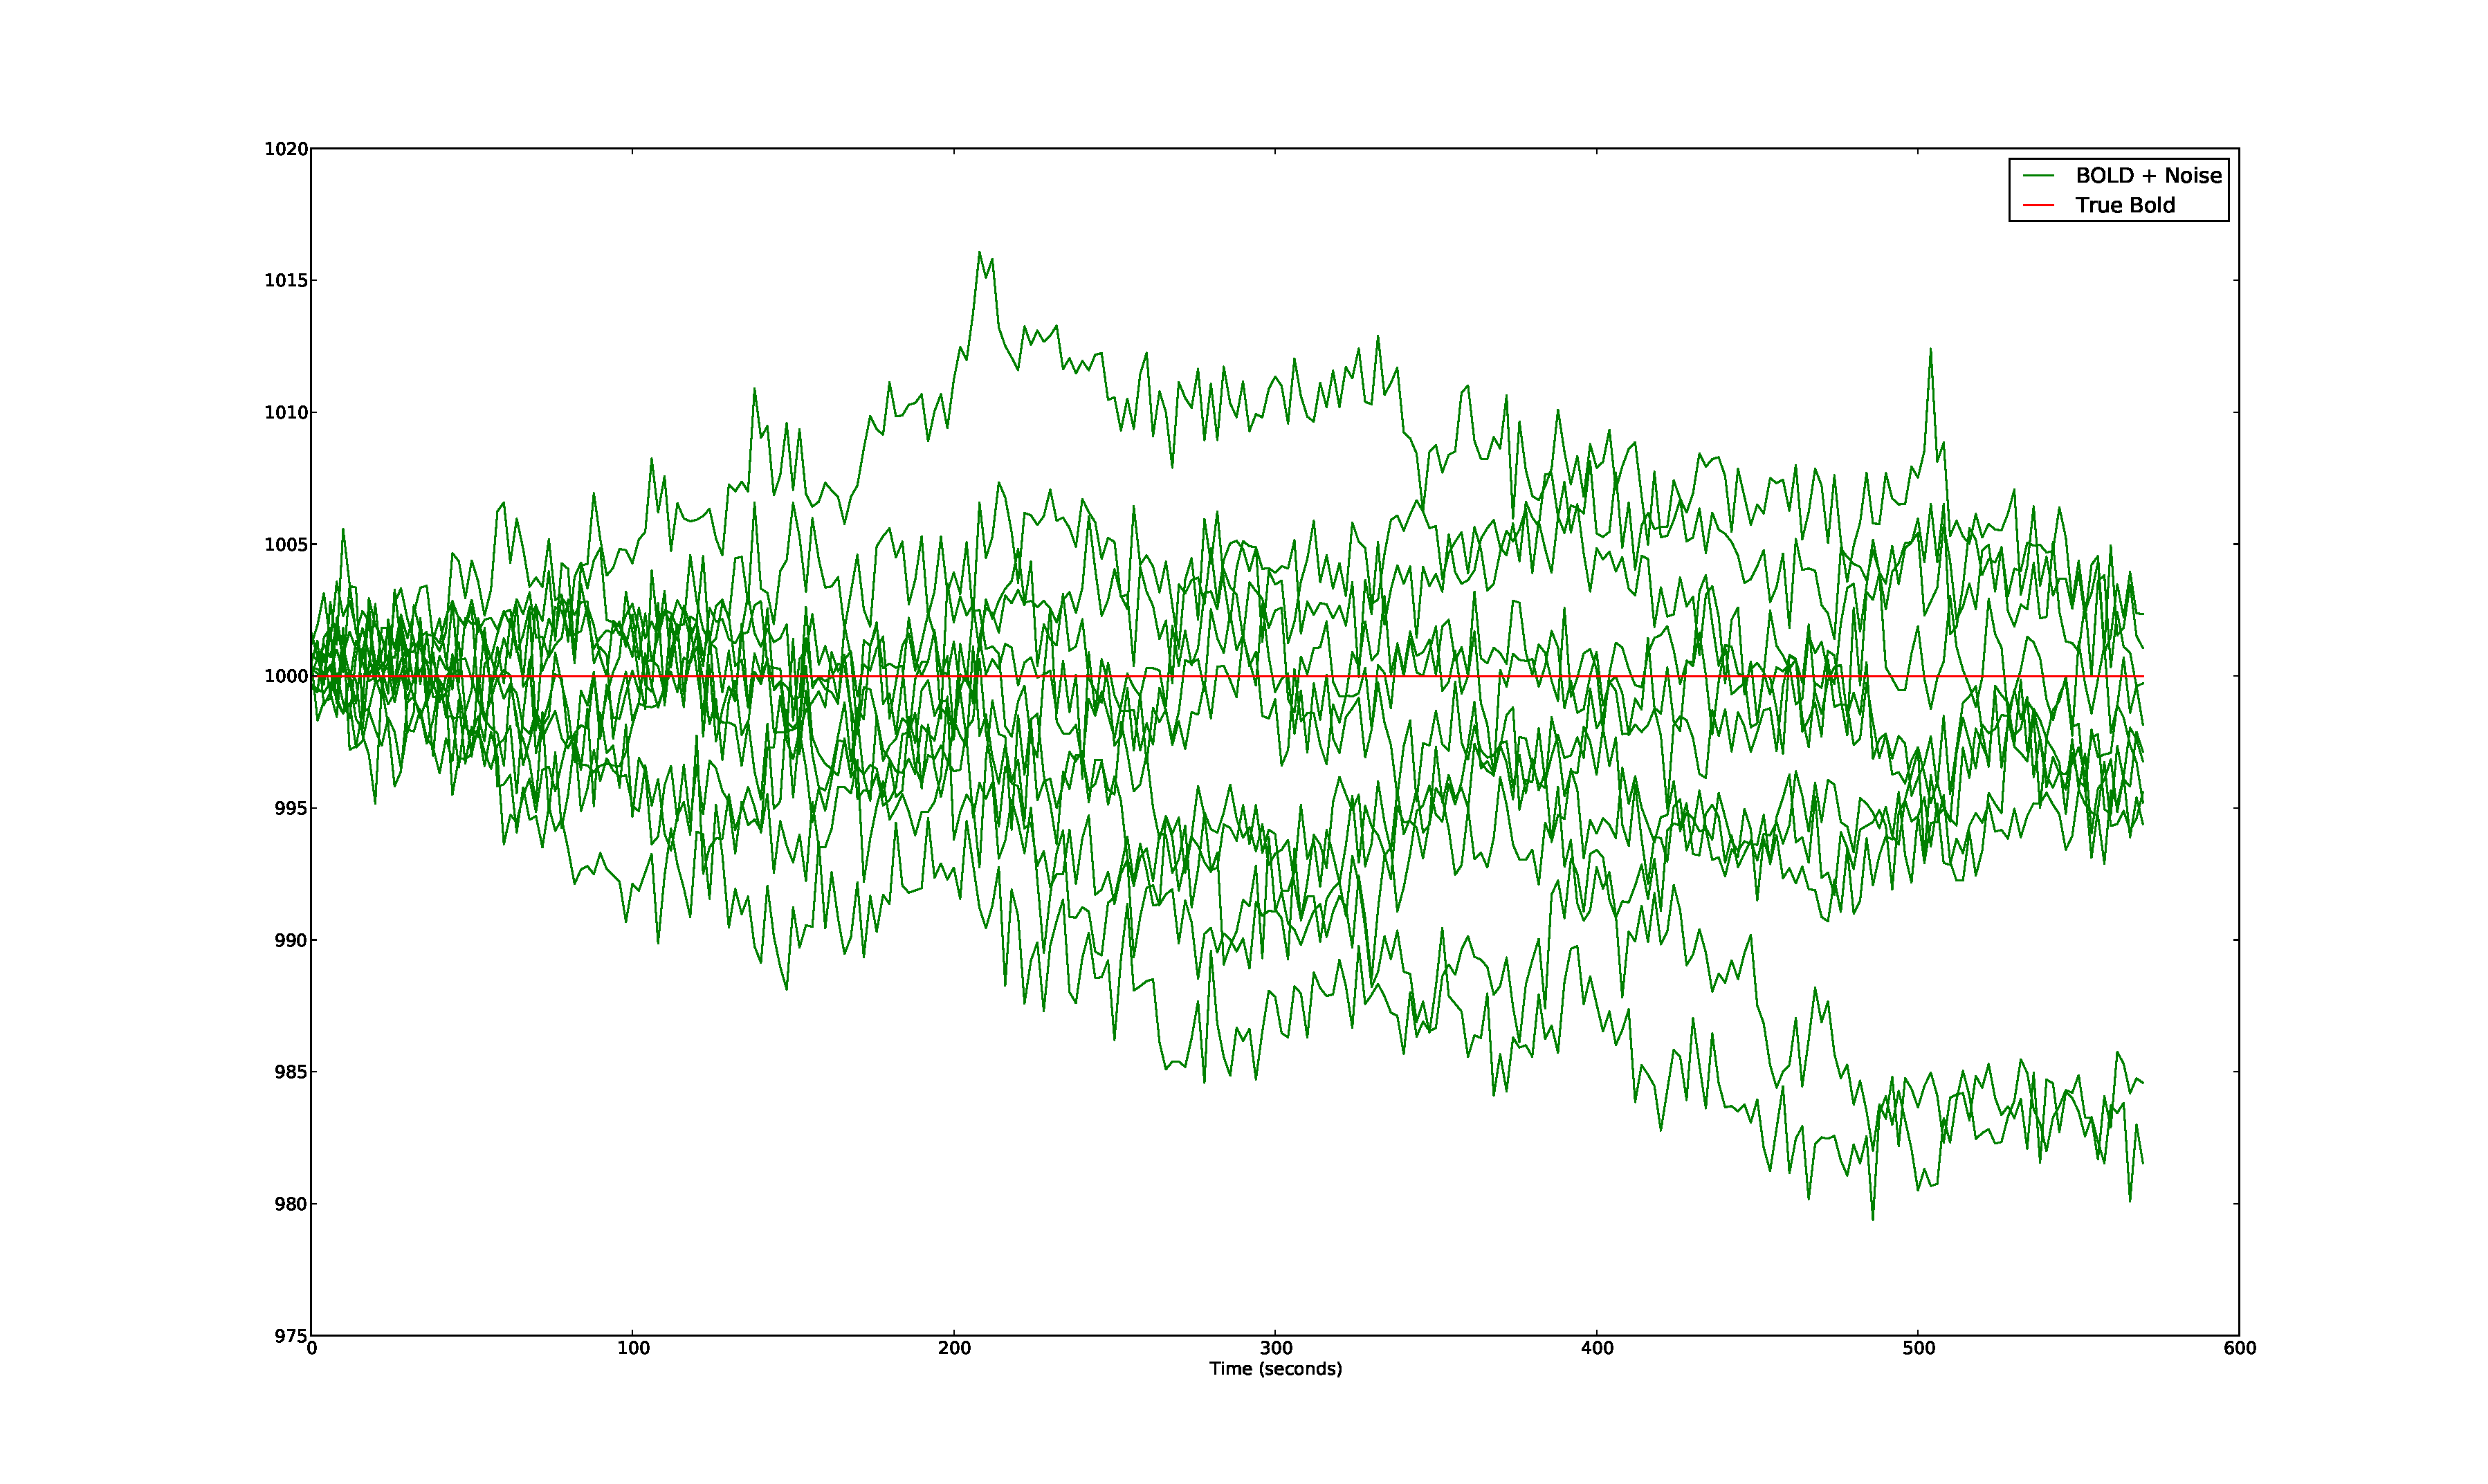
\includegraphics[clip=true,trim=6cm 3cm 6cm 3cm,height=7cm]{images/realization_noiseonly}
\caption{Time-series lacking any real signal. With, $\sigma_x = .01, \sigma_y=.005$}
\label{fig:NoiseOnly}
\end{figure}

\begin{figure}[H]
\centering
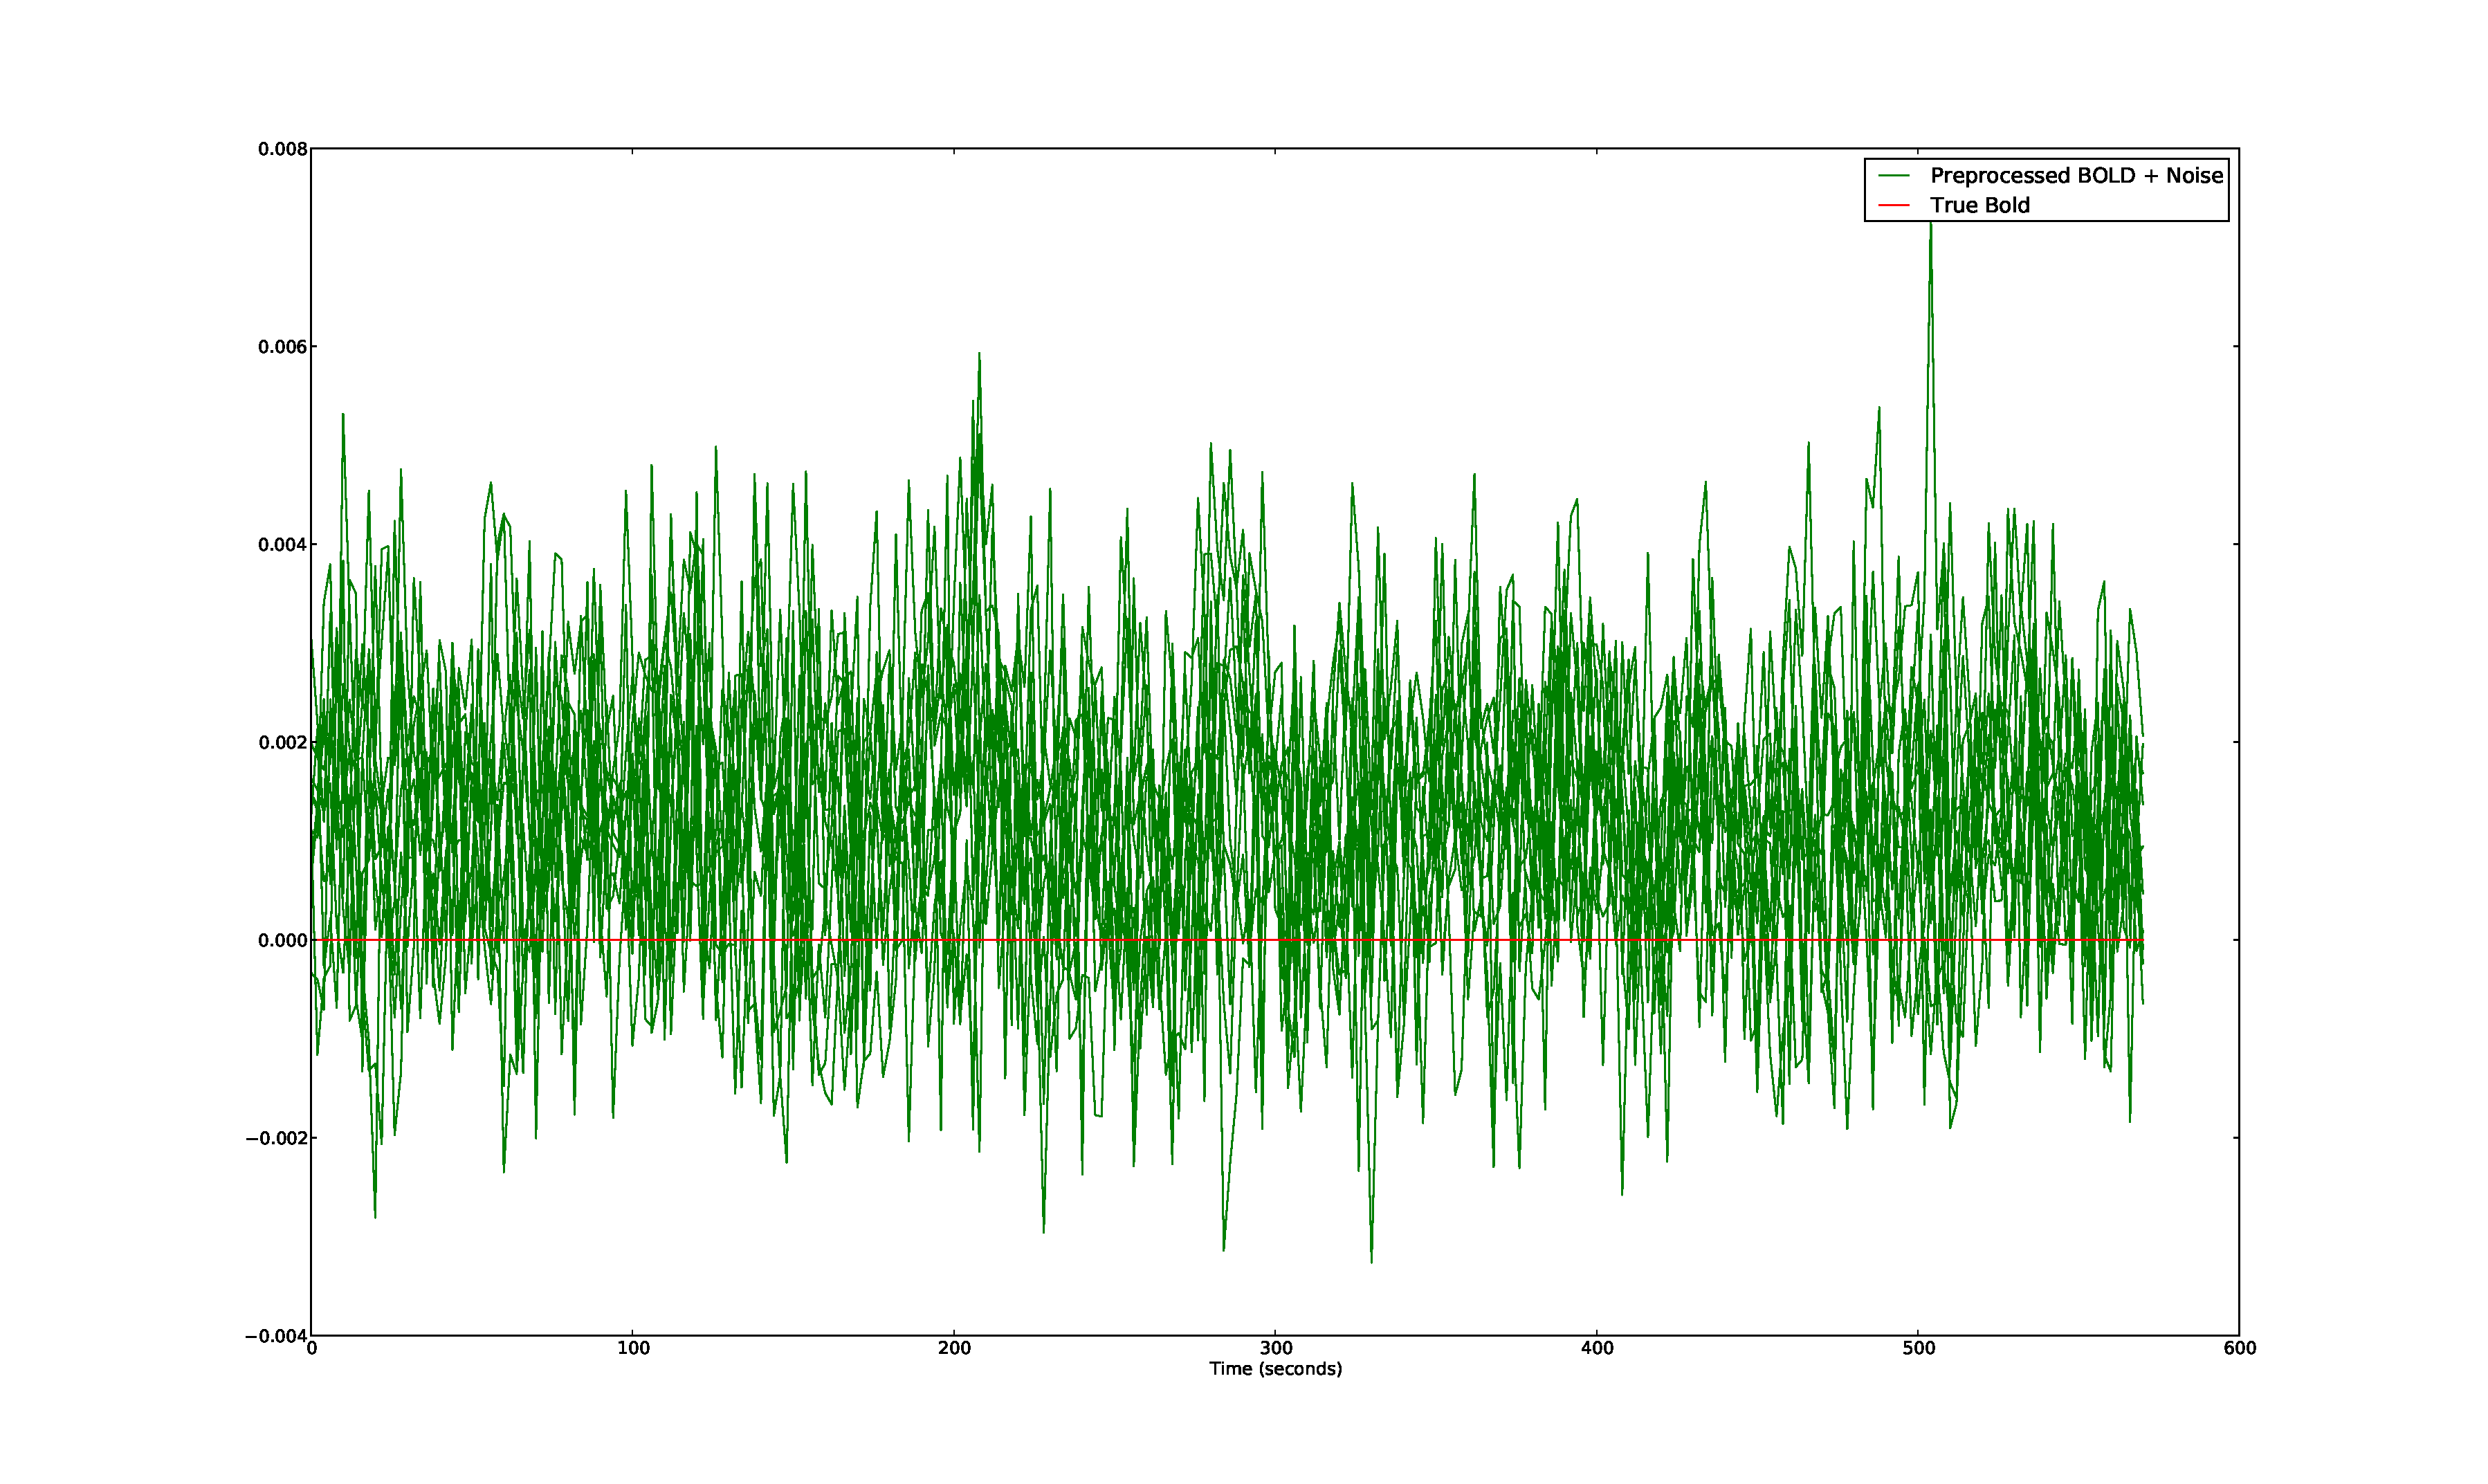
\includegraphics[clip=true,trim=6cm 3cm 6cm 3cm,height=7cm]{images/preprocessed_noiseonly}
\caption{A comparison of the preprocessed signals for the signal-free case. (
$\sigma_y = .01, \sigma_x = .005$)}
\label{fig:PreprocessedNoiseOnly}
\end{figure}

\begin{table}[t]
\centering
\begin{tabular}{|c | c | c | c | c | c | c | c | c |}
\hline 
$\tau_0$ & $\alpha$ & $E_0$    & $V_0$    & $\tau_s$ & $\tau_f$ & $\epsilon$  &  $\sqrt{MSR}$   \\
\hline 
1.0324 & 0.33211 & 0.34058 & 0.03012 & 1.40665 & 2.52079 & 0.5311 &   0.00167  \\
 0.98189 & 0.33047 & 0.3386 & 0.03014 & 1.45707 & 2.47232 & 0.45049 & 0.00159   \\
 1.0429 & 0.33224 & 0.34124 & 0.02946 & 1.4618 & 2.49245 & 0.43012 &  0.00165   \\
 1.02054 & 0.3321 & 0.33484 & 0.02586 & 1.45848 & 2.48741 & 0.4193 &  0.00151   \\
 1.0565 & 0.33405 & 0.33758 & 0.02791 & 1.43784 & 2.52545 & 0.47517 & 0.00152   \\
 1.01867 & 0.33528 & 0.33918 & 0.02782 & 1.48345 & 2.49605 & 0.44209 &0.00156   \\
 1.051 & 0.33038 & 0.33837 & 0.02985 & 1.47651 & 2.48621 & 0.42719 &  0.00159   \\
 1.00281 & 0.32929 & 0.33988 & 0.0298 & 1.43519 & 2.49256 & 0.48899 & 0.00164   \\
 1.00893 & 0.33273 & 0.33982 & 0.0289 & 1.42903 & 2.49754 & 0.45688 & 0.00168   \\
 1.01289 & 0.33275 & 0.3376 & 0.02997 & 1.41188 & 2.49881 & 0.50628 & 0.00183   \\
 1.10247 & 0.33371 & 0.3419 & 0.02939 & 1.43774 & 2.53384 & 0.44079 & 0.00195   \\
\hline                                                                  
1.03009 & 0.33228 & 0.33905 & 0.02902 & 1.44506 & 2.50031 & 0.46076 & 0.00165 \\
\hline
\end{tabular}
\caption{Estimated Parameters on 11 different runs with low noise and no signal present.}
\label{tab:NoiseOnlyResults} 
\end{table}

\begin{figure}[H]
\centering
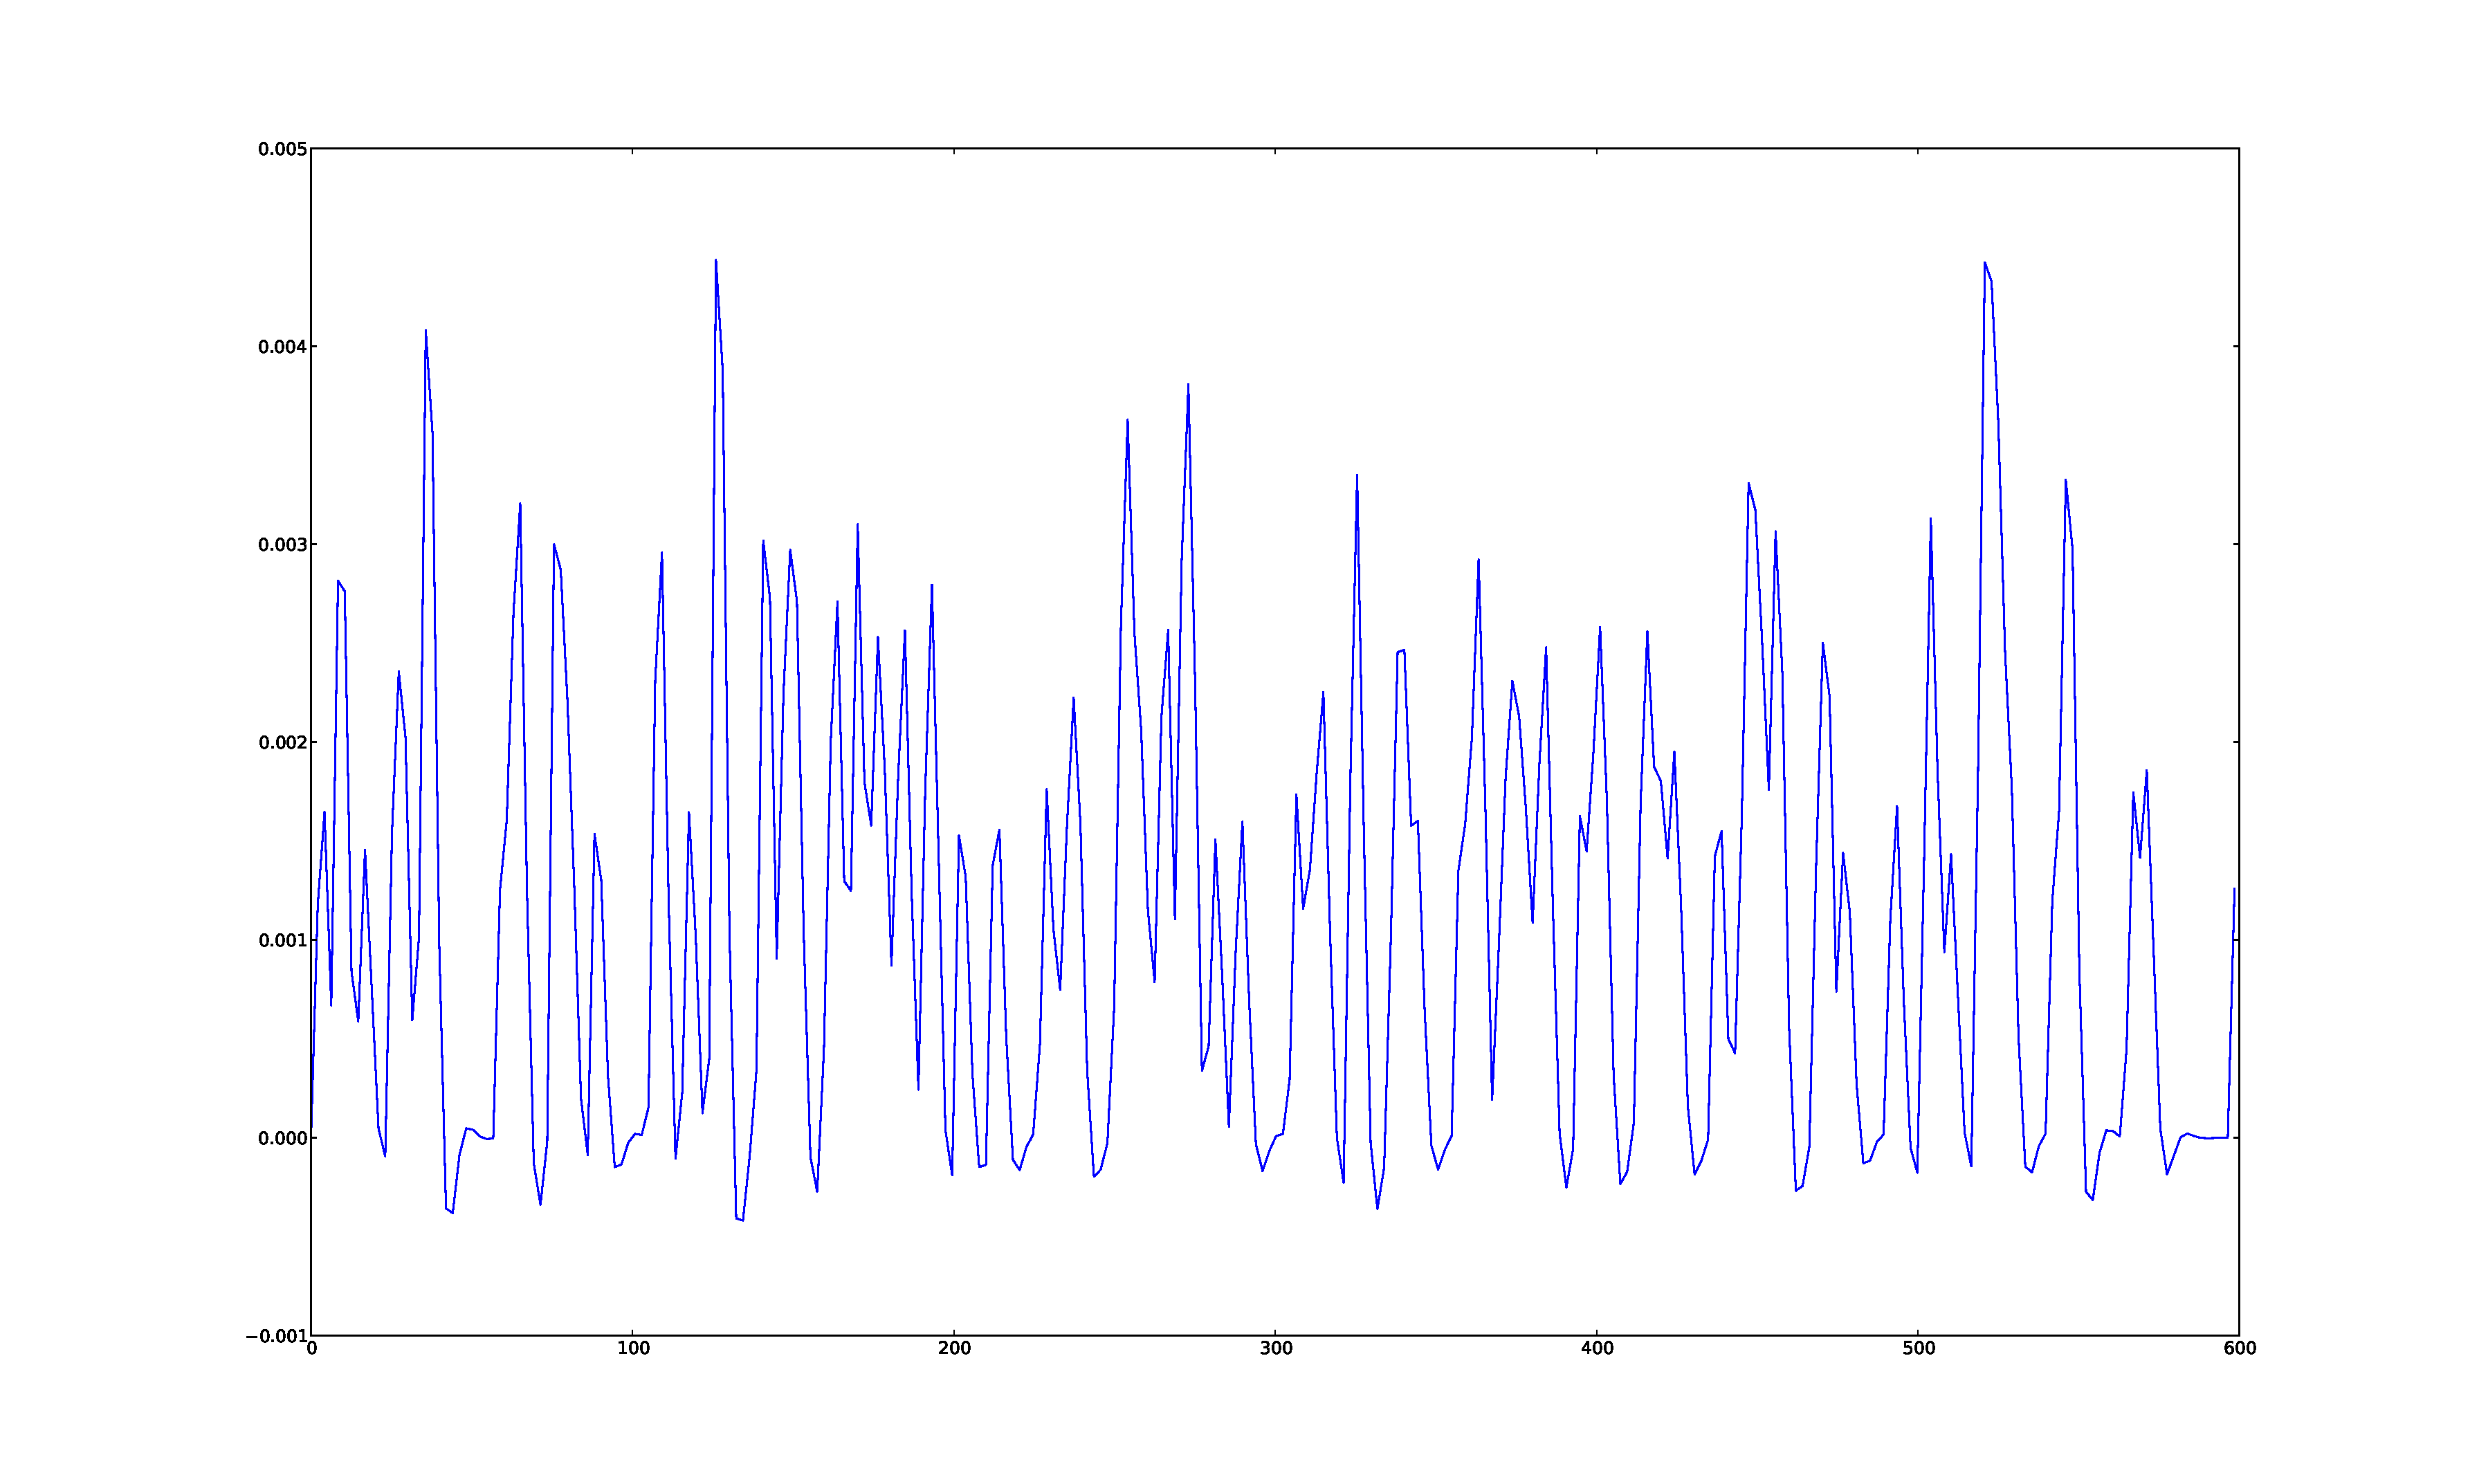
\includegraphics[clip=true,trim=6cm 3cm 6cm 3cm,height=9cm]{images/fits_noiseonly}
\caption{Fits to the non-active, low noise signal. Note that the line is thick because all
the fits overlap. This is all 11 fitted lines.}
\label{fig:fits_noiseonly}
\end{figure}

\begin{figure}[H]
\centering
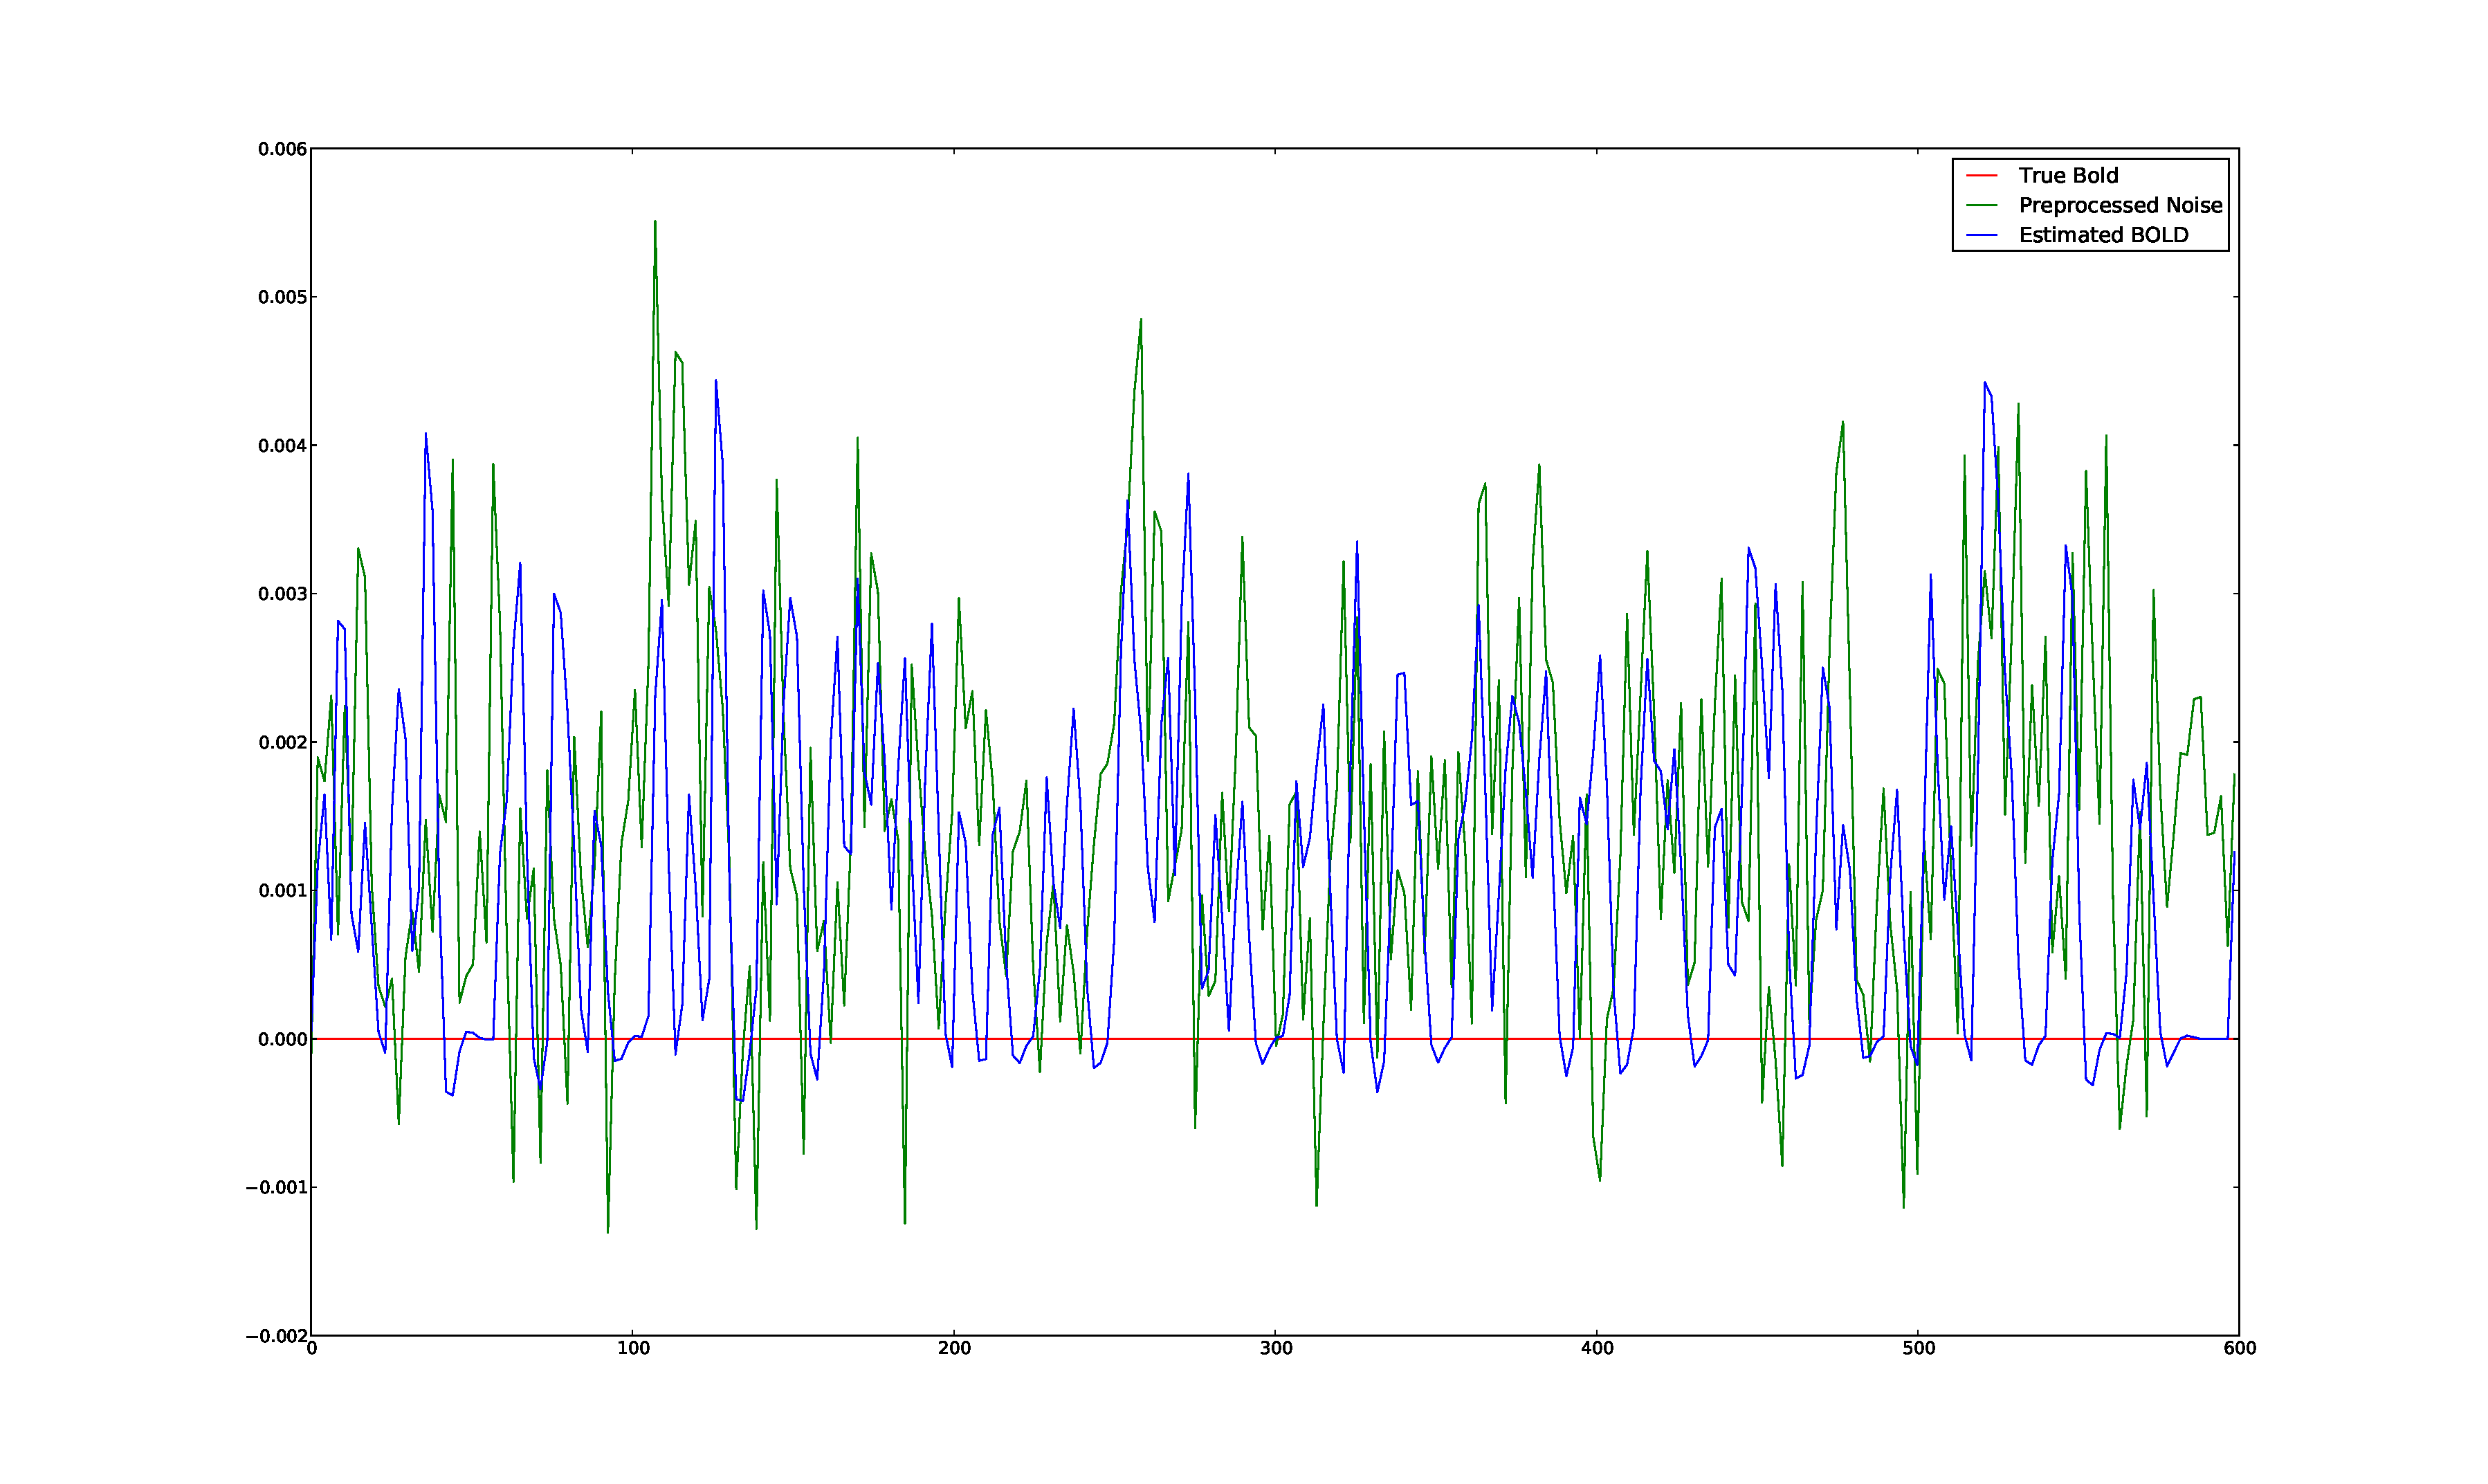
\includegraphics[clip=true,trim=6cm 3cm 6cm 3cm,height=9cm]{images/justnoise_fit_0}
\caption{Fit from a single particle filter run, with the noise input. }
\label{fig:justnoise_fit_0}
\end{figure} %uses allnoise/ALLNOISE-0-w0

\begin{figure}[H]
\centering
\subfigure[$\tau_0$, $\alpha$, $E_0$, $V_0$]
{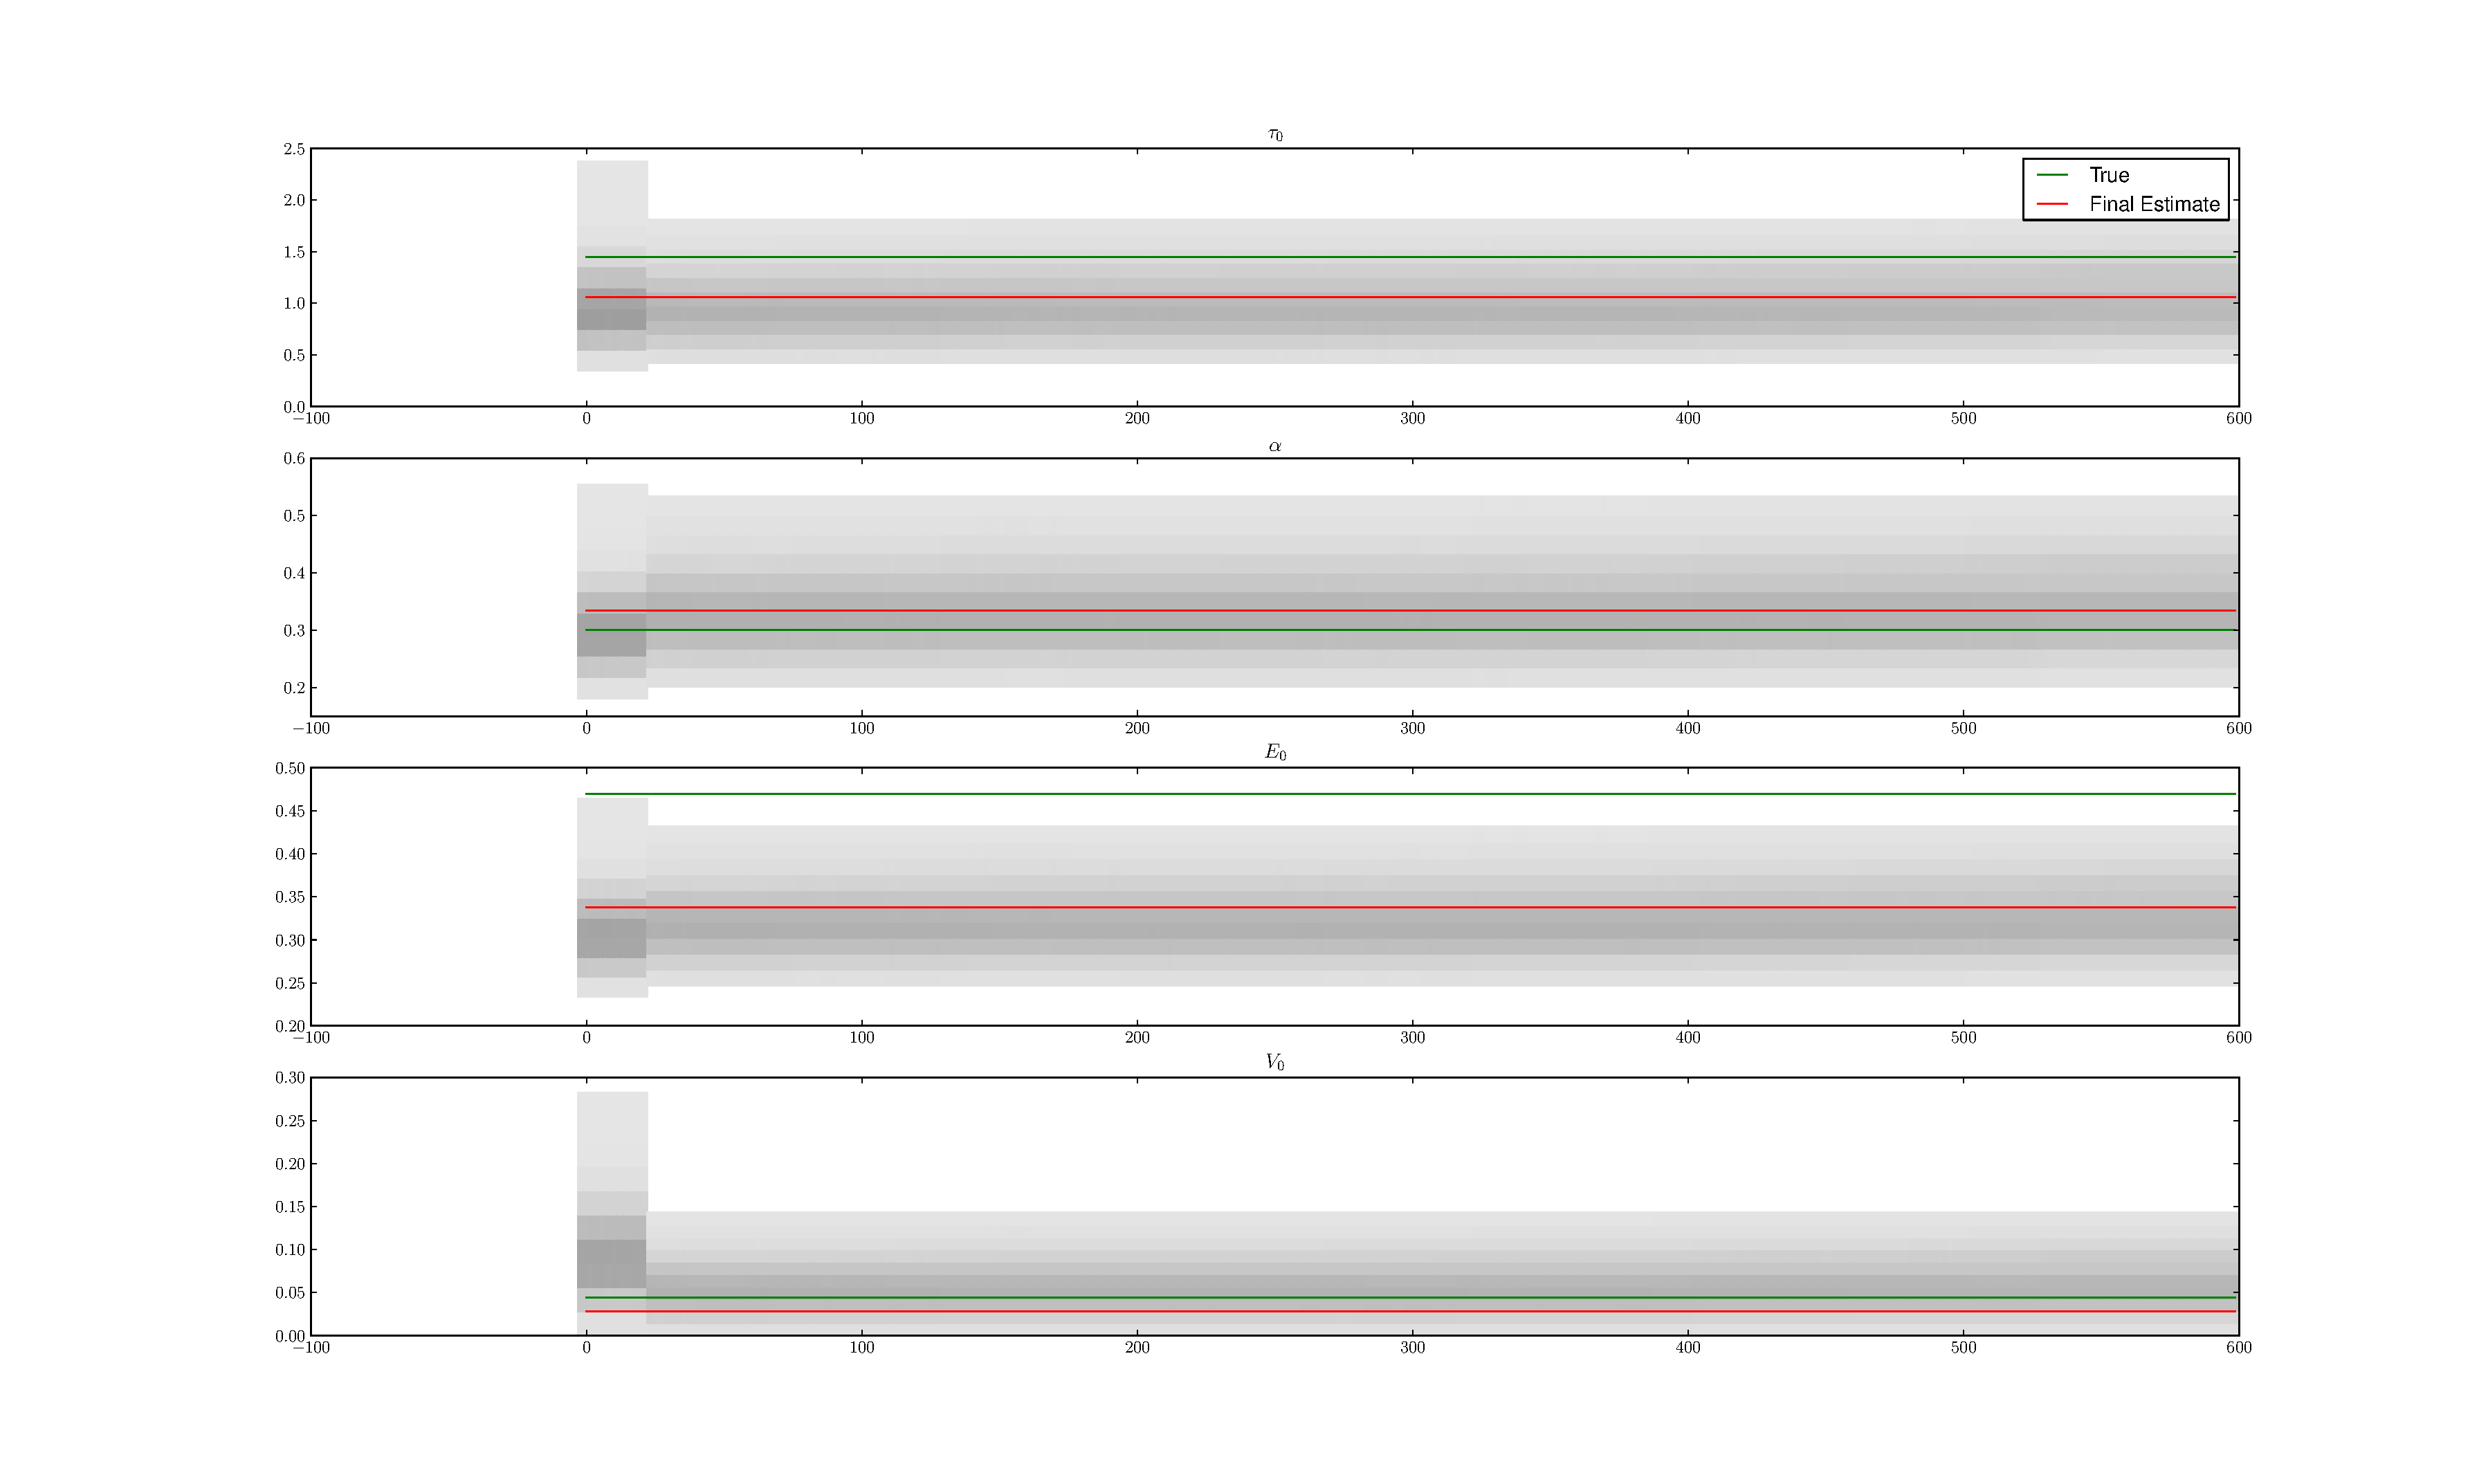
\includegraphics[clip=true,trim=6cm 2cm 6cm 3cm, height=9cm]{images/justnoise_hist_1}}\\
\end{figure}

\begin{figure}[H]
\centering
\subfigure[$\tau_s$, $\tau_f$, $\epsilon$, $V$] 
{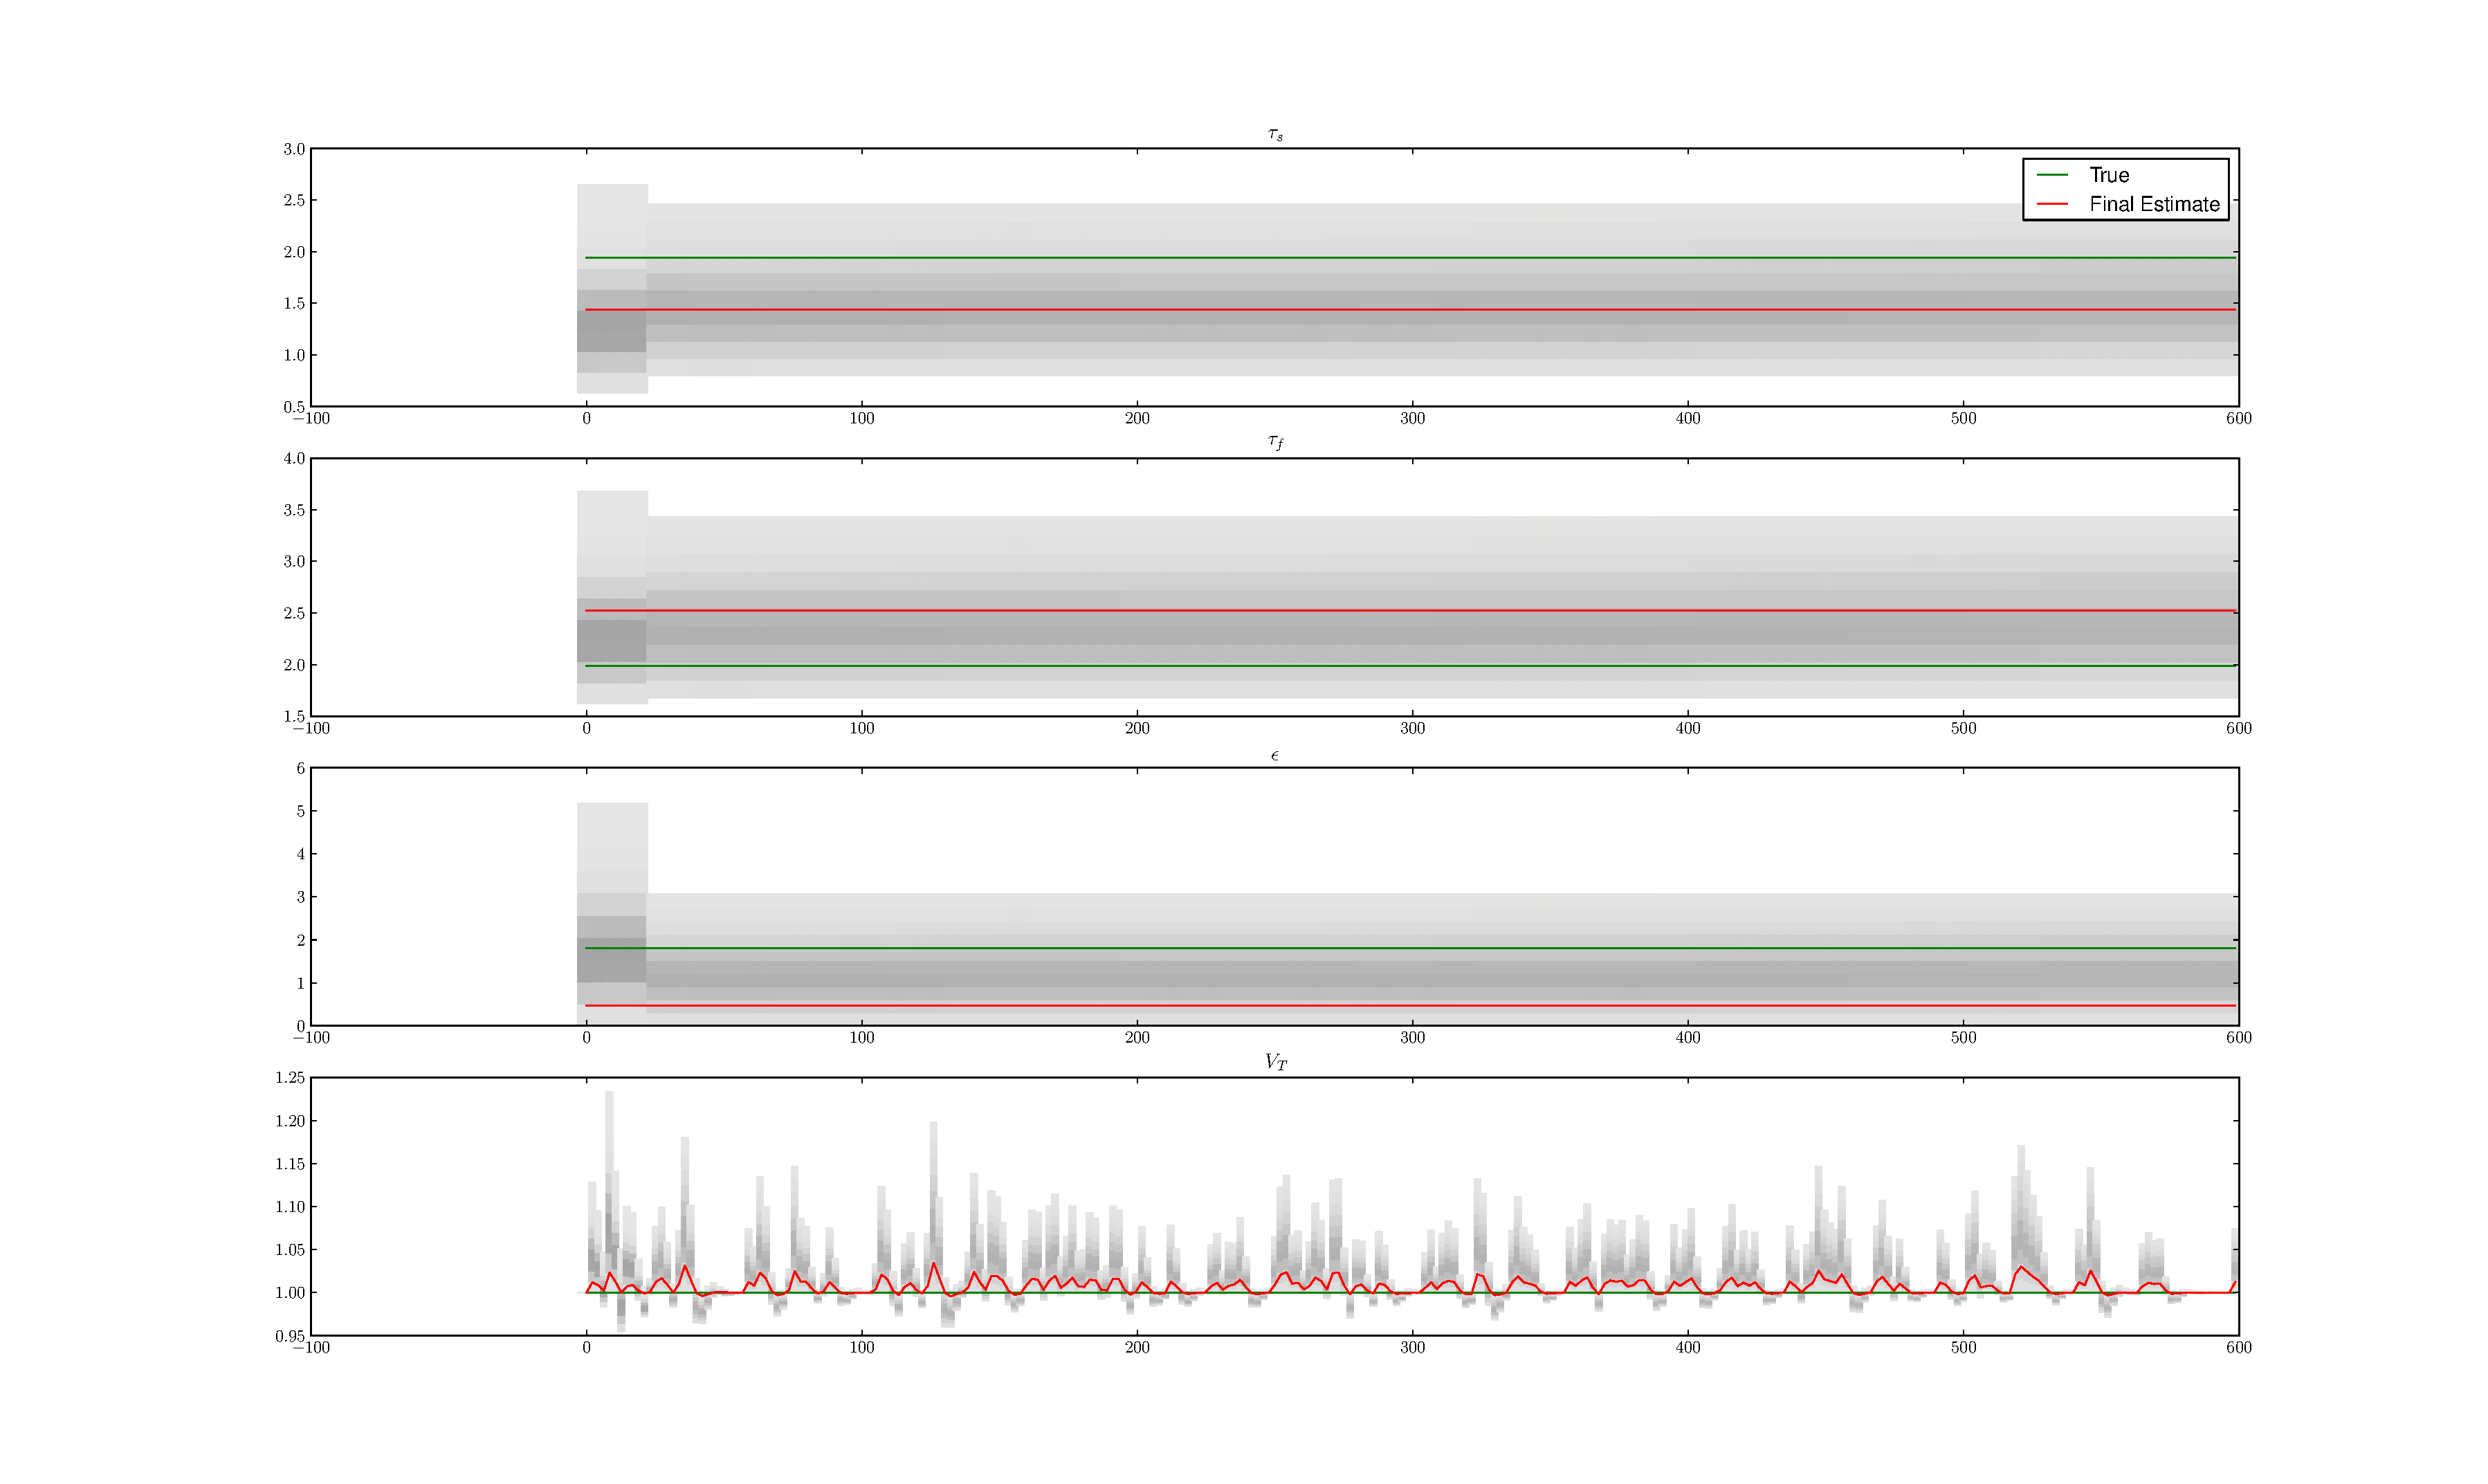
\includegraphics[clip=true,trim=6cm 2cm 6cm 3cm, height=9cm]{images/justnoise_hist_2}}\\
\end{figure}

\begin{figure}[H]
\centering
\subfigure[$Q$, $S$, $F$, $BOLD$ ]
{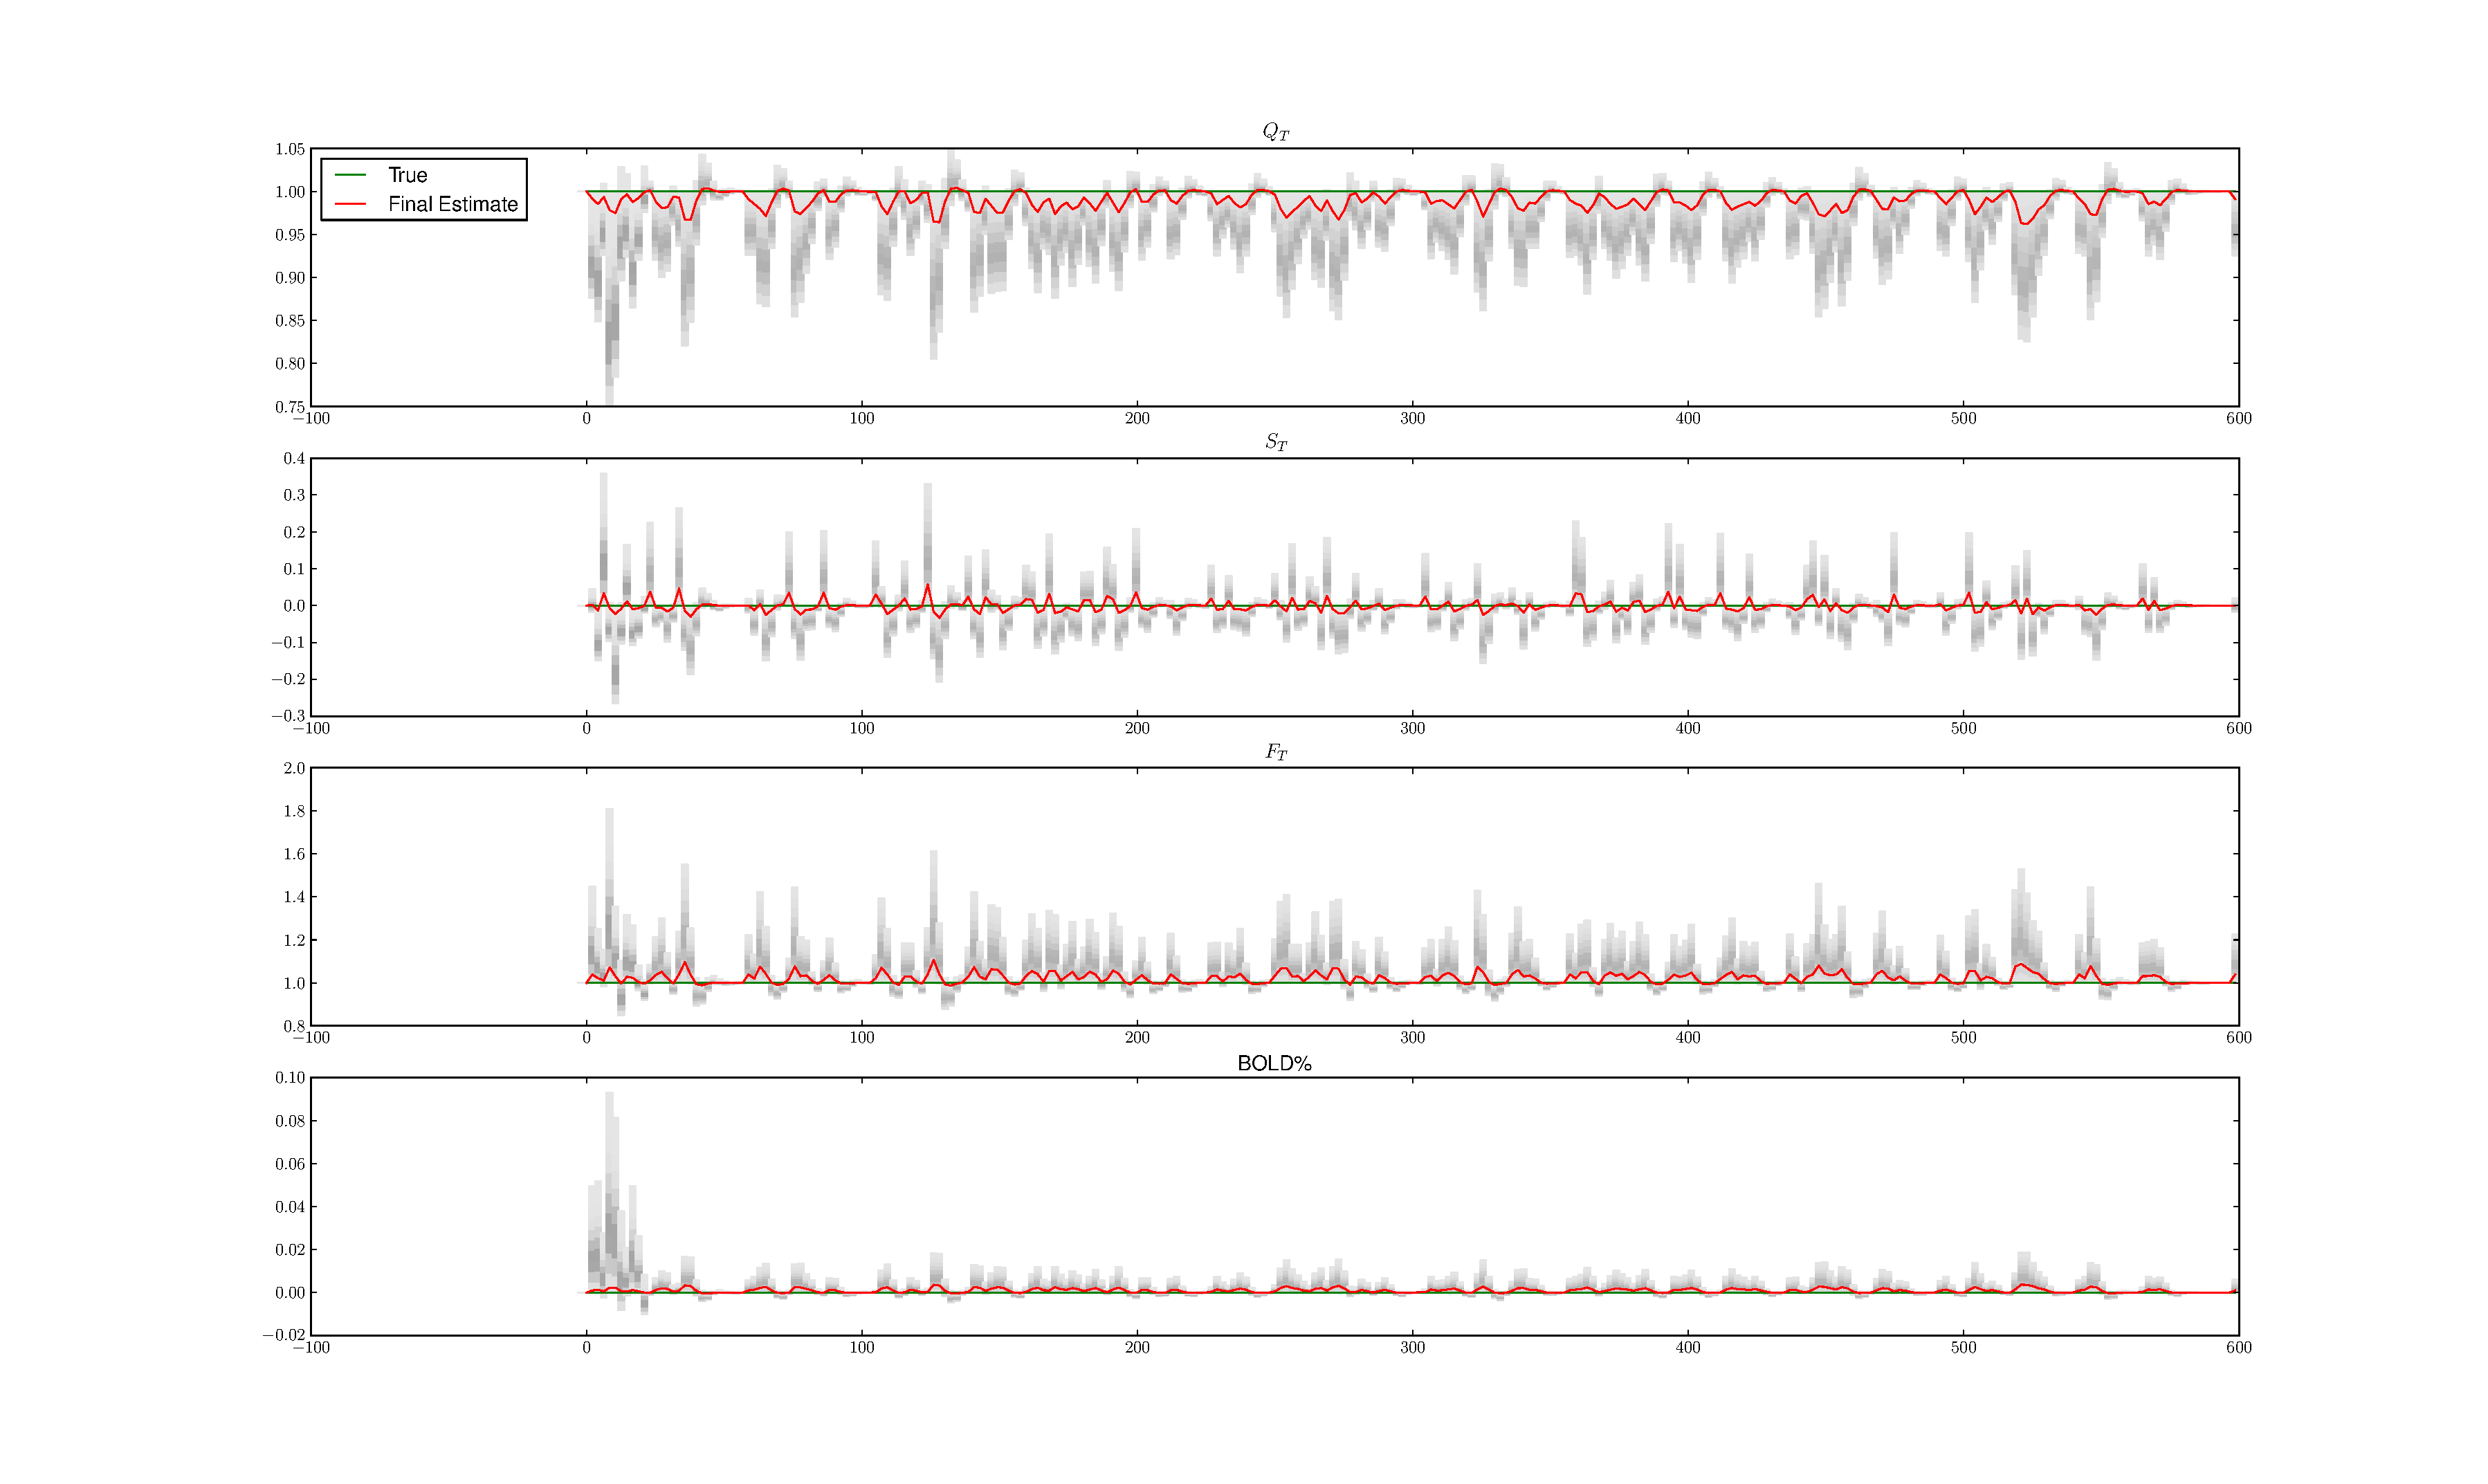
\includegraphics[clip=true,trim=6cm 2cm 6cm 3cm, height=9cm]{images/justnoise_hist_3}}
\caption{Converging histogram for parameters when the signal consists purely of low level noise. 
Same run as \autoref{fig:justnoise_fit_0}}
\label{fig:JustNoiseConvergence}
\end{figure}

The data shows that the parameters have not taken any visible turns into
unrealistic territory; individual parameters will not be a distinguishing factor
in determining the validity of the model. Additionally the residual 
also appears to be lower than the residual of the low noise simulation from earlier. 
The precision with which the convergence occurred is actually the best seen in any
simulation.  The reason for the low error is that the overall
signal is significantly smaller than any other simulation in this thesis.
The peaks never even 1\% difference, with most staying even below .5\% 
(\autoref{fig:PreprocessedNoiseOnly}). Because the stayed 
well within the range of $.005$, which is the standard deviation of the weighting function
the particles did not ever get substantially different weights. Thus, the reason
the fits are in such agreement is that no particles gained increased weight, and so
no convergence occurred at all, as further shown by \autoref{fig:JustNoiseConvergence}. 
This is good evidence that a per time-series weighting function could benefit
even out the convergence rate; and thus allow better determination between signals
like this and low noise case from earlier.
Thus we have now seen how the particle filter responds when the signal is completely
random and low level, however there is also some possibility that the signal will
be random, yet active. Thus one more test is necessary; time series with no 
underlying signal (as far as responding stimuli) but with enough noise to 
actually be considered a signal. 

%NO SIGNAL, VERY HIGH NOISE
\subsection{Pure Noise, High Magnitude}
\label{sec:PureNoiseHighMag}
To determine how the particle filter will respond to active, yet unrelated
portions of the brain, in this section random data will again be used, but
with even higher standard deviations. To simulate this case another
pure noise signal was generated using a $\sigma_x$ of $.1$ and a $\sigma_y$ of $.05$.

As before, the convergence all seems to follow a similar path, leaving almost no
variance in the estimated time series (\autoref{fig:fits_noiseonly_high}). Now, however
the peaks are comparable to peaks in a real timeseries. Interestingly the algorithm
suffered from almost constant particle deprivation, meaning that the heuristic
for rescuing the particle filter from particle deprivation, discussed in
\autoref{sec:Resampling} in fact was working against the proper course of action. 
 The proper course of action in this case would be for the particle filter to fail,
 since no particle can really properly estimate a random sequence. When this mechanism
 was removed, all 11 runs stopped due to particle deprivation (all weights hit zero). 
 The problem with allowing particle deprivation to occur is that it can \emph{rarely}
 occur if the prior happens to not be dense enough in the area of the solution. Thus,
 there is an issue of false positives vs. false negatives. A middle ground, such as 
 allowing deprivation to occur if the recovery mechanism has already triggered once
 may be an acceptable compromise, however it would be difficult to strike the 
 right balance. Instead, for the purposes here, I depend on other methods, described
 later, evaluate if the results were reasonable or not. 

\begin{figure}[H]
\centering
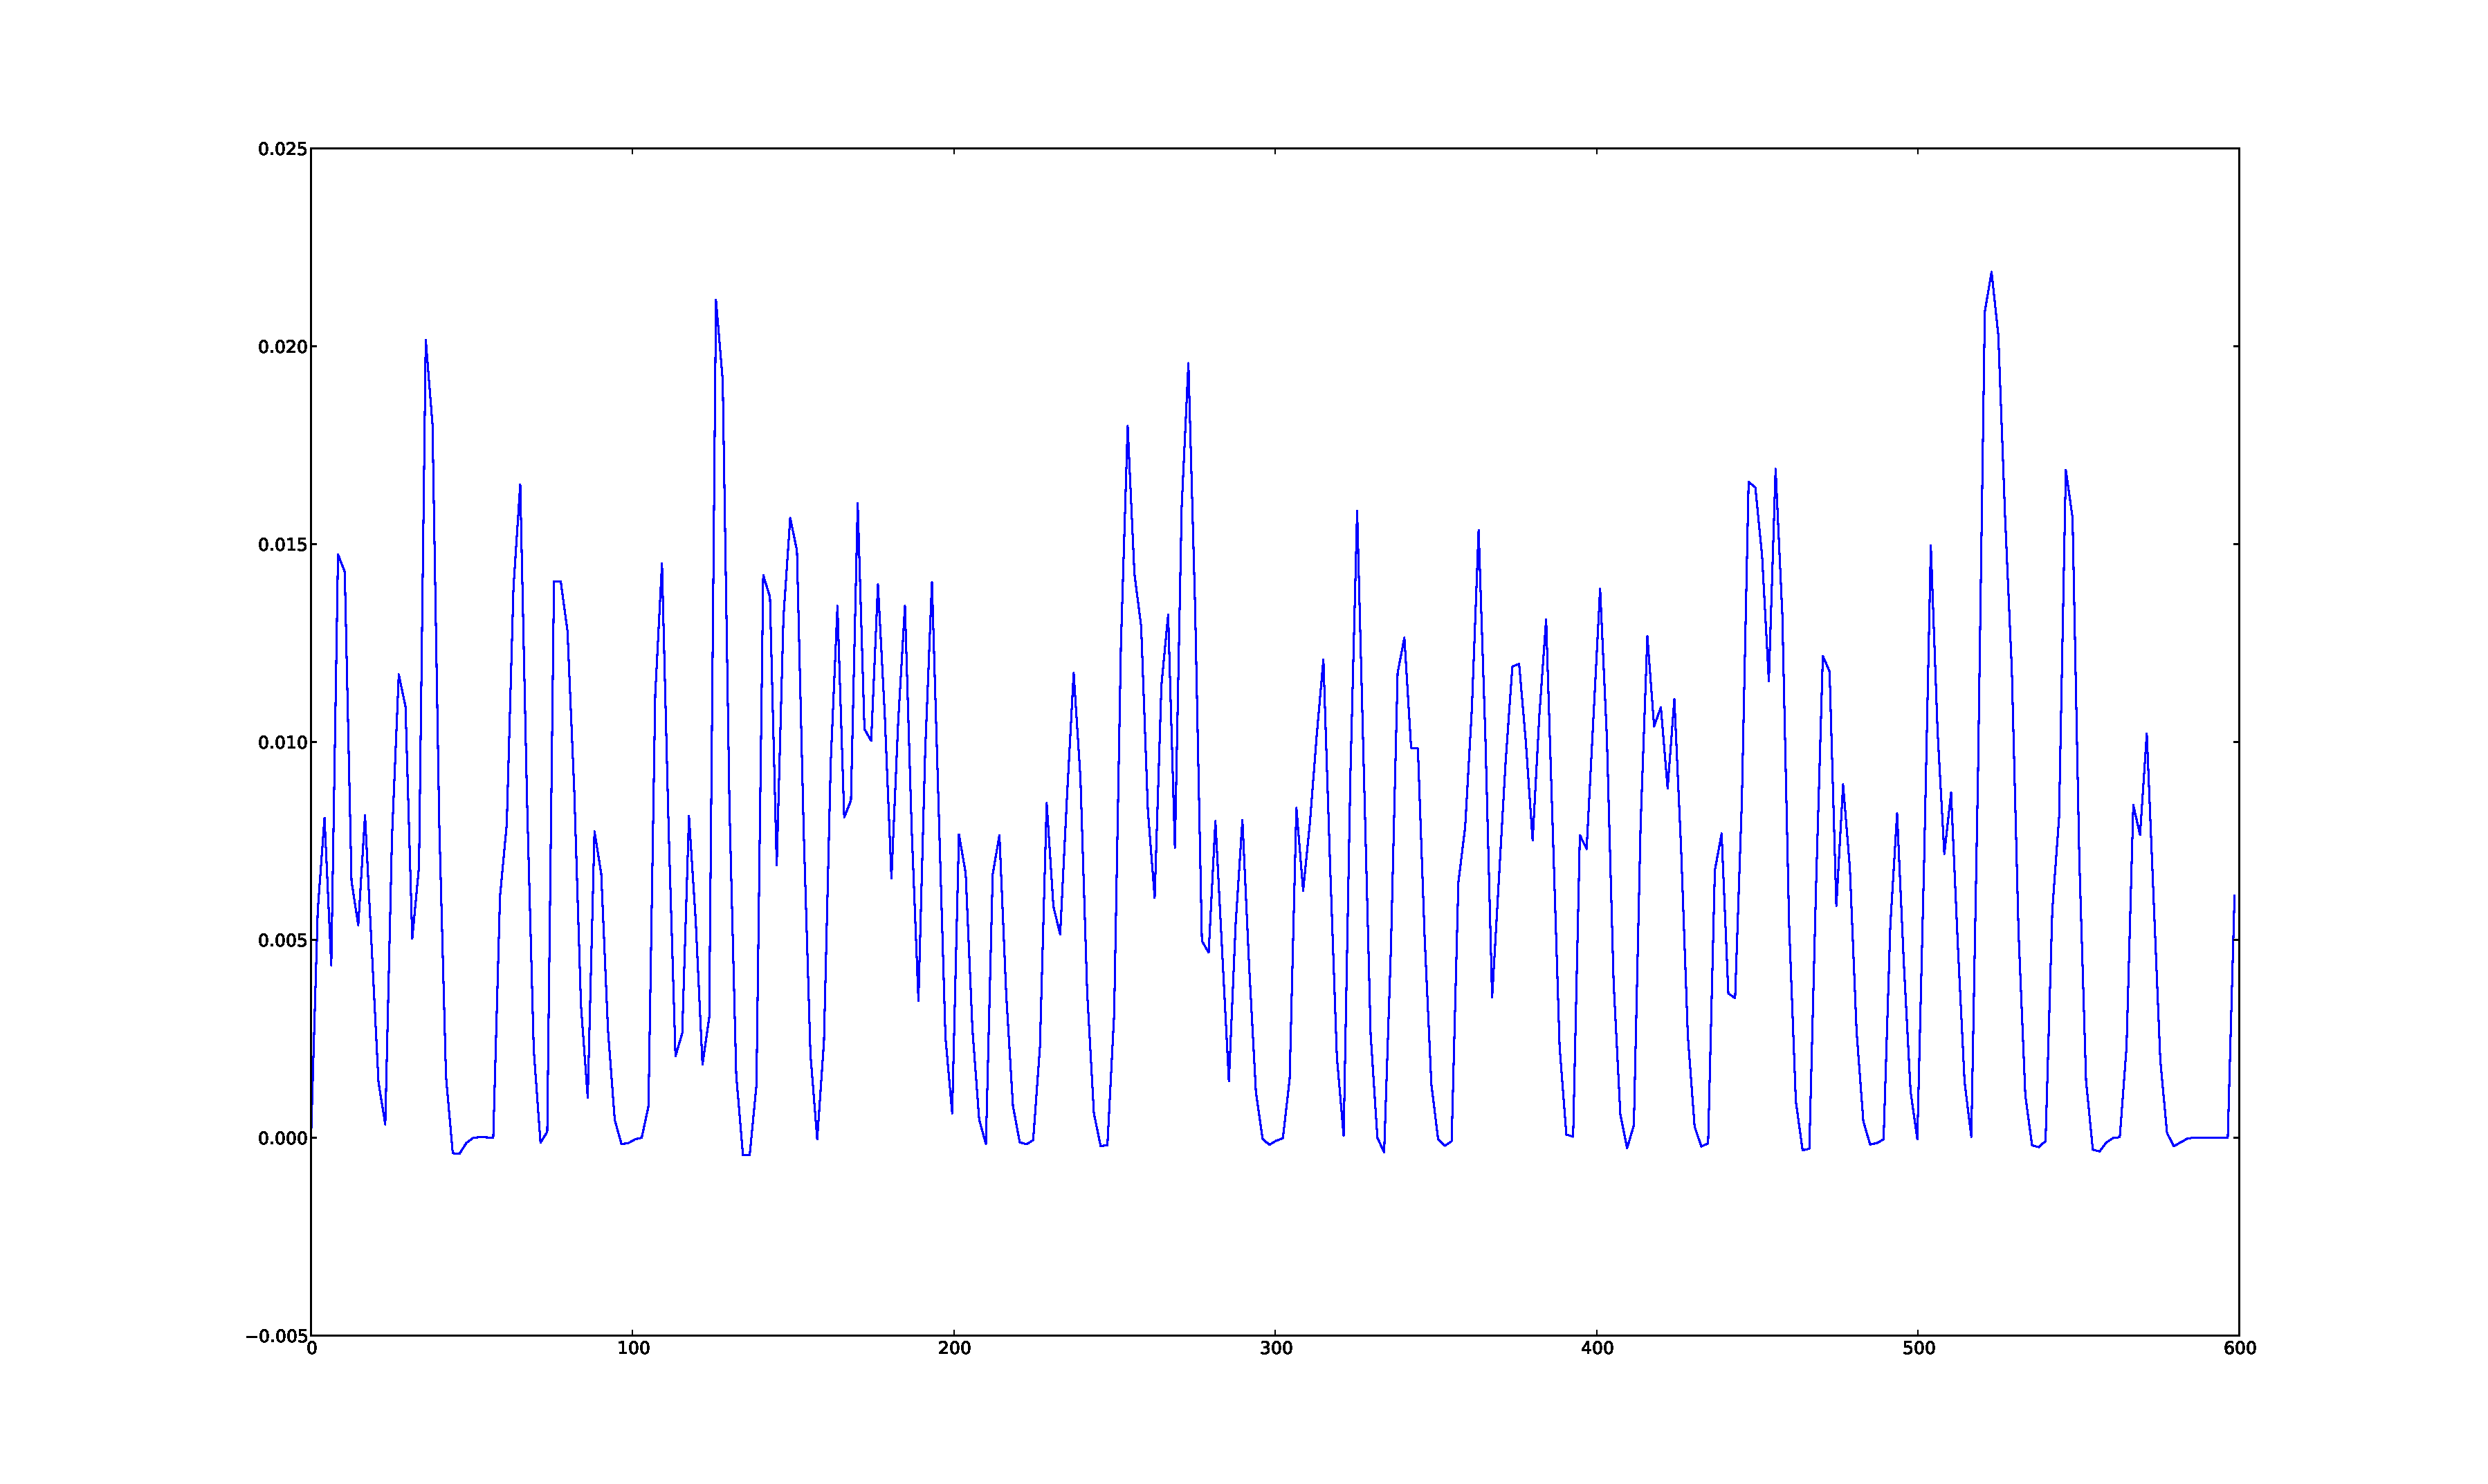
\includegraphics[clip=true,trim=6cm 3cm 6cm 3cm,height=9cm]{images/fits_noiseonly_high}
\caption{Fits to the non-active, high noise signal. Note that the line is thick because all
the fits overlap. This is all 11 fitted lines.}
\label{fig:fits_noiseonly_high}
\end{figure}

\begin{figure}[H]
\centering
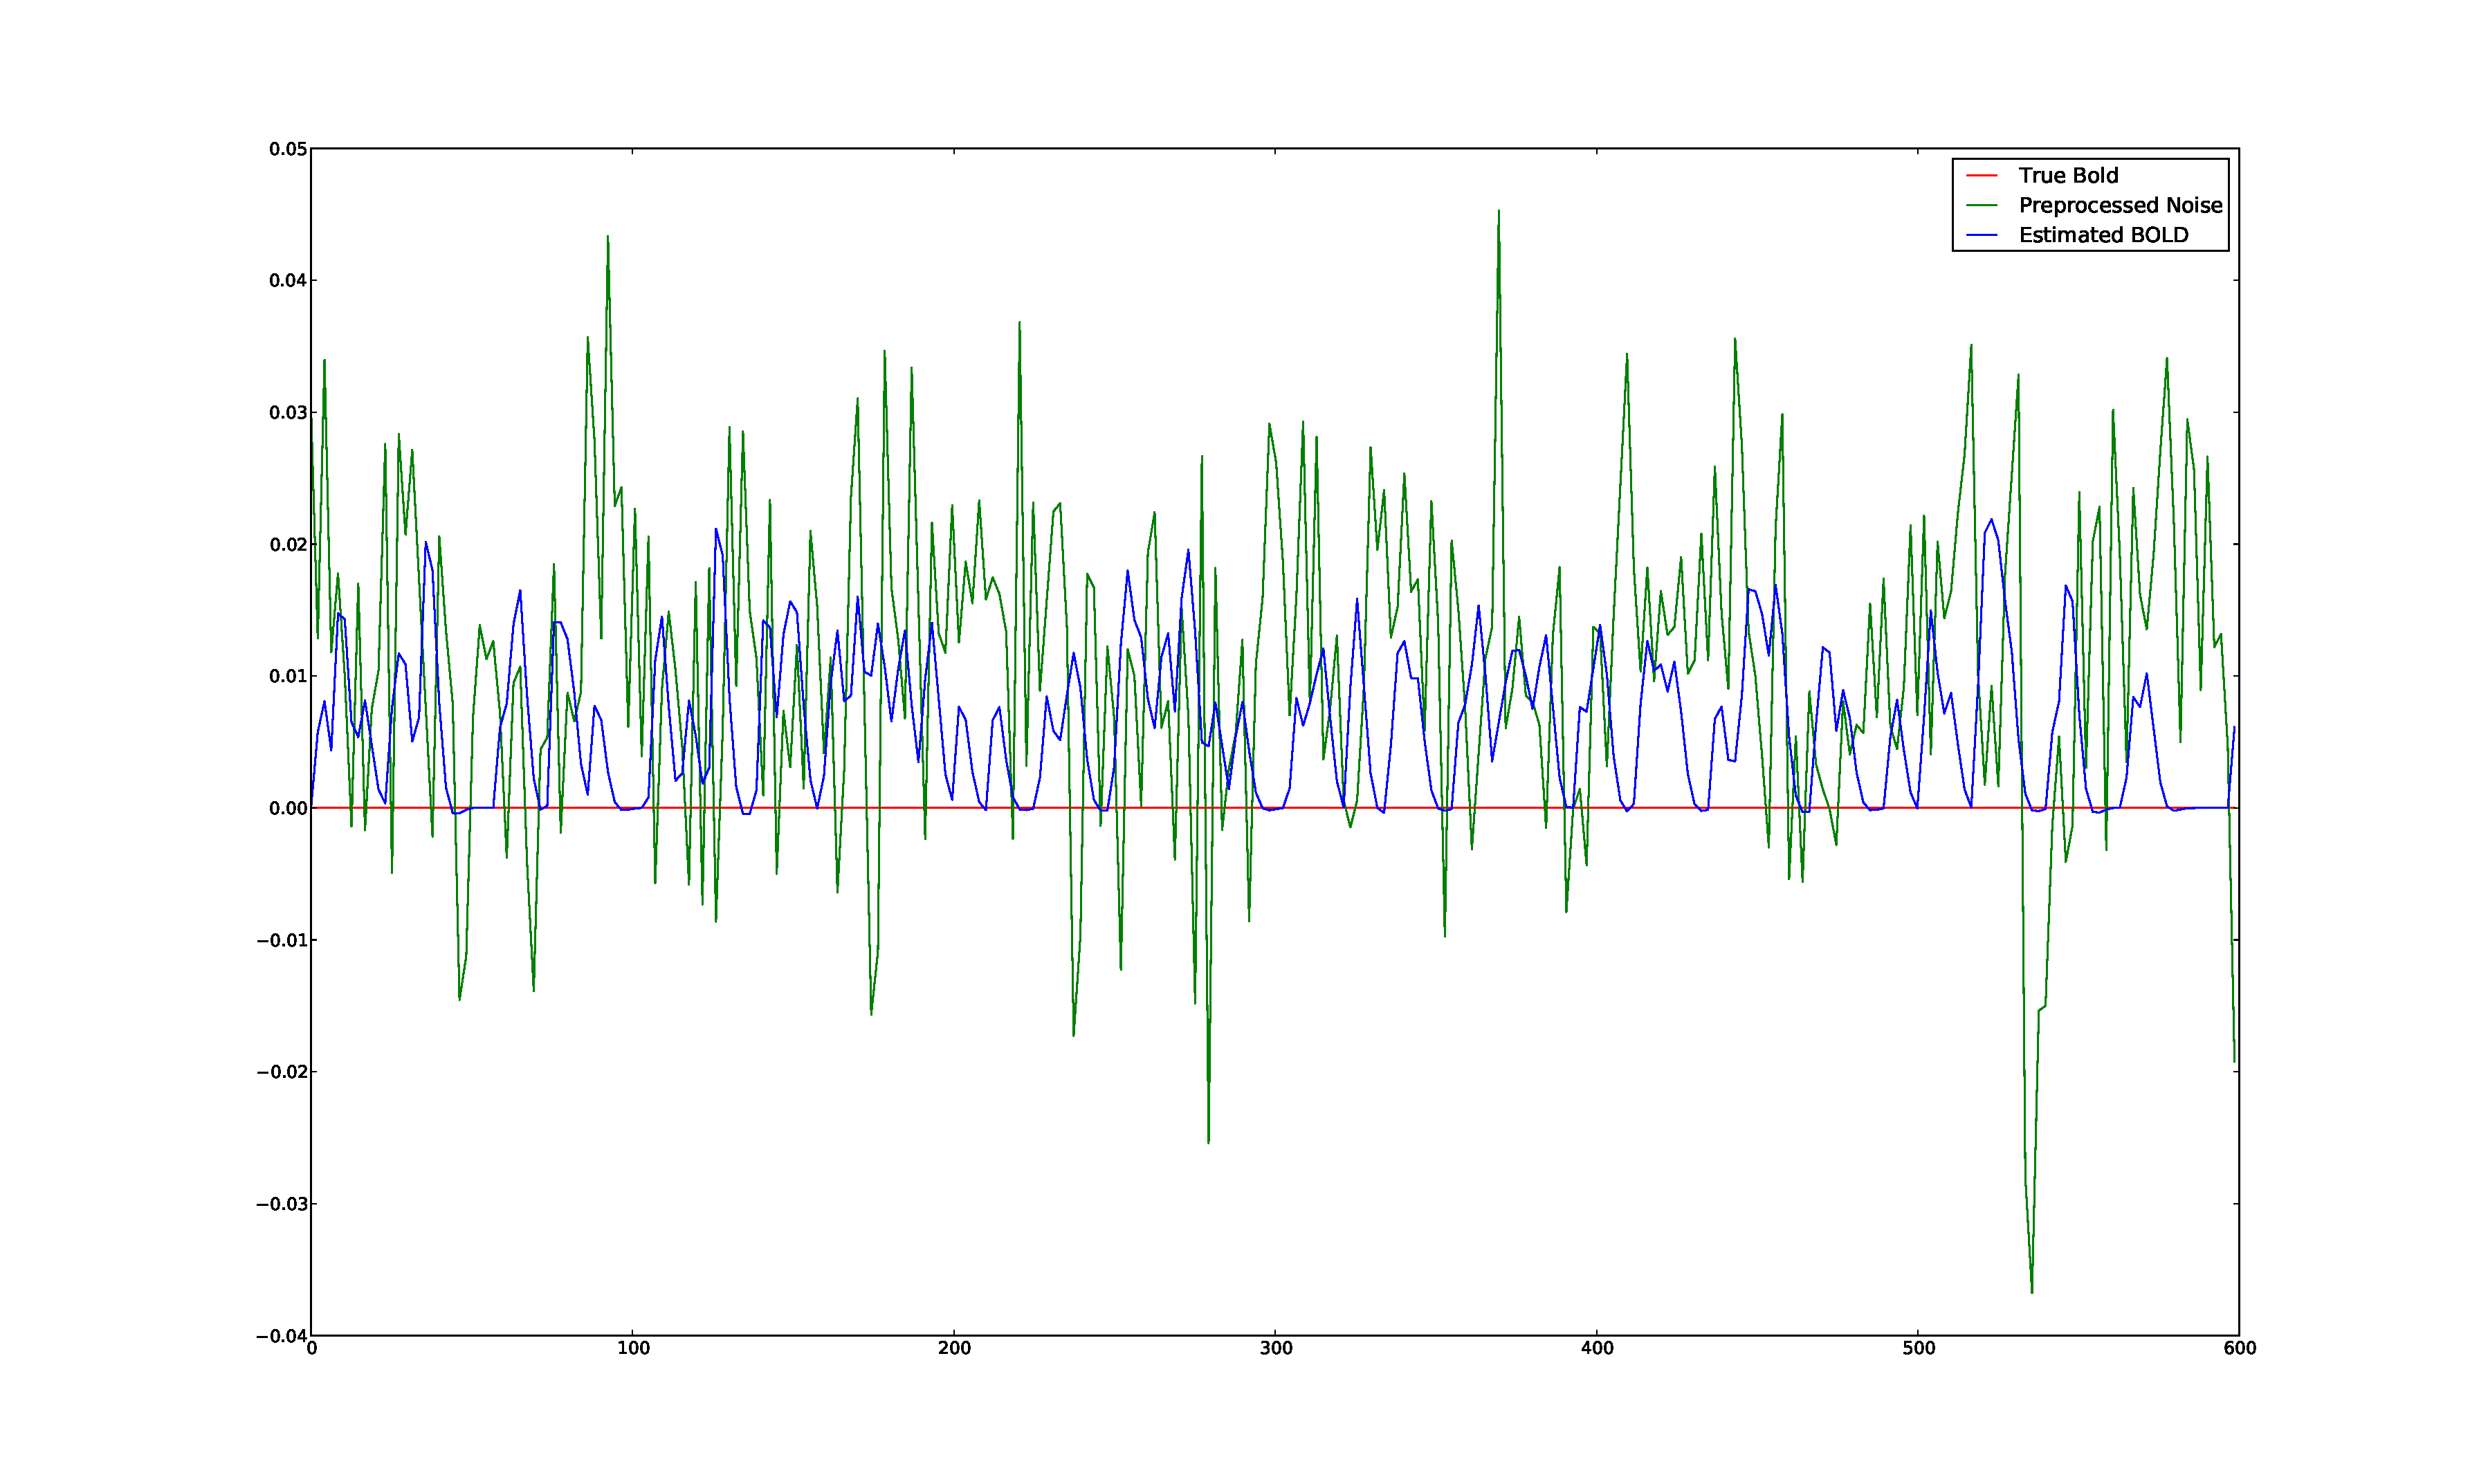
\includegraphics[clip=true,trim=6cm 3cm 6cm 3cm,height=9cm]{images/justbignoise_fit_0}
\caption{Fit from a single particle filter run, with the noise input. }
\label{fig:justbignoise_fit_0}
\end{figure} %uses allnoise/ALLNOISE-0-w0

%\begin{figure}[H]
%\centering
%\subfigure[$\tau_0$, $\alpha$, $E_0$, $V_0$]
%{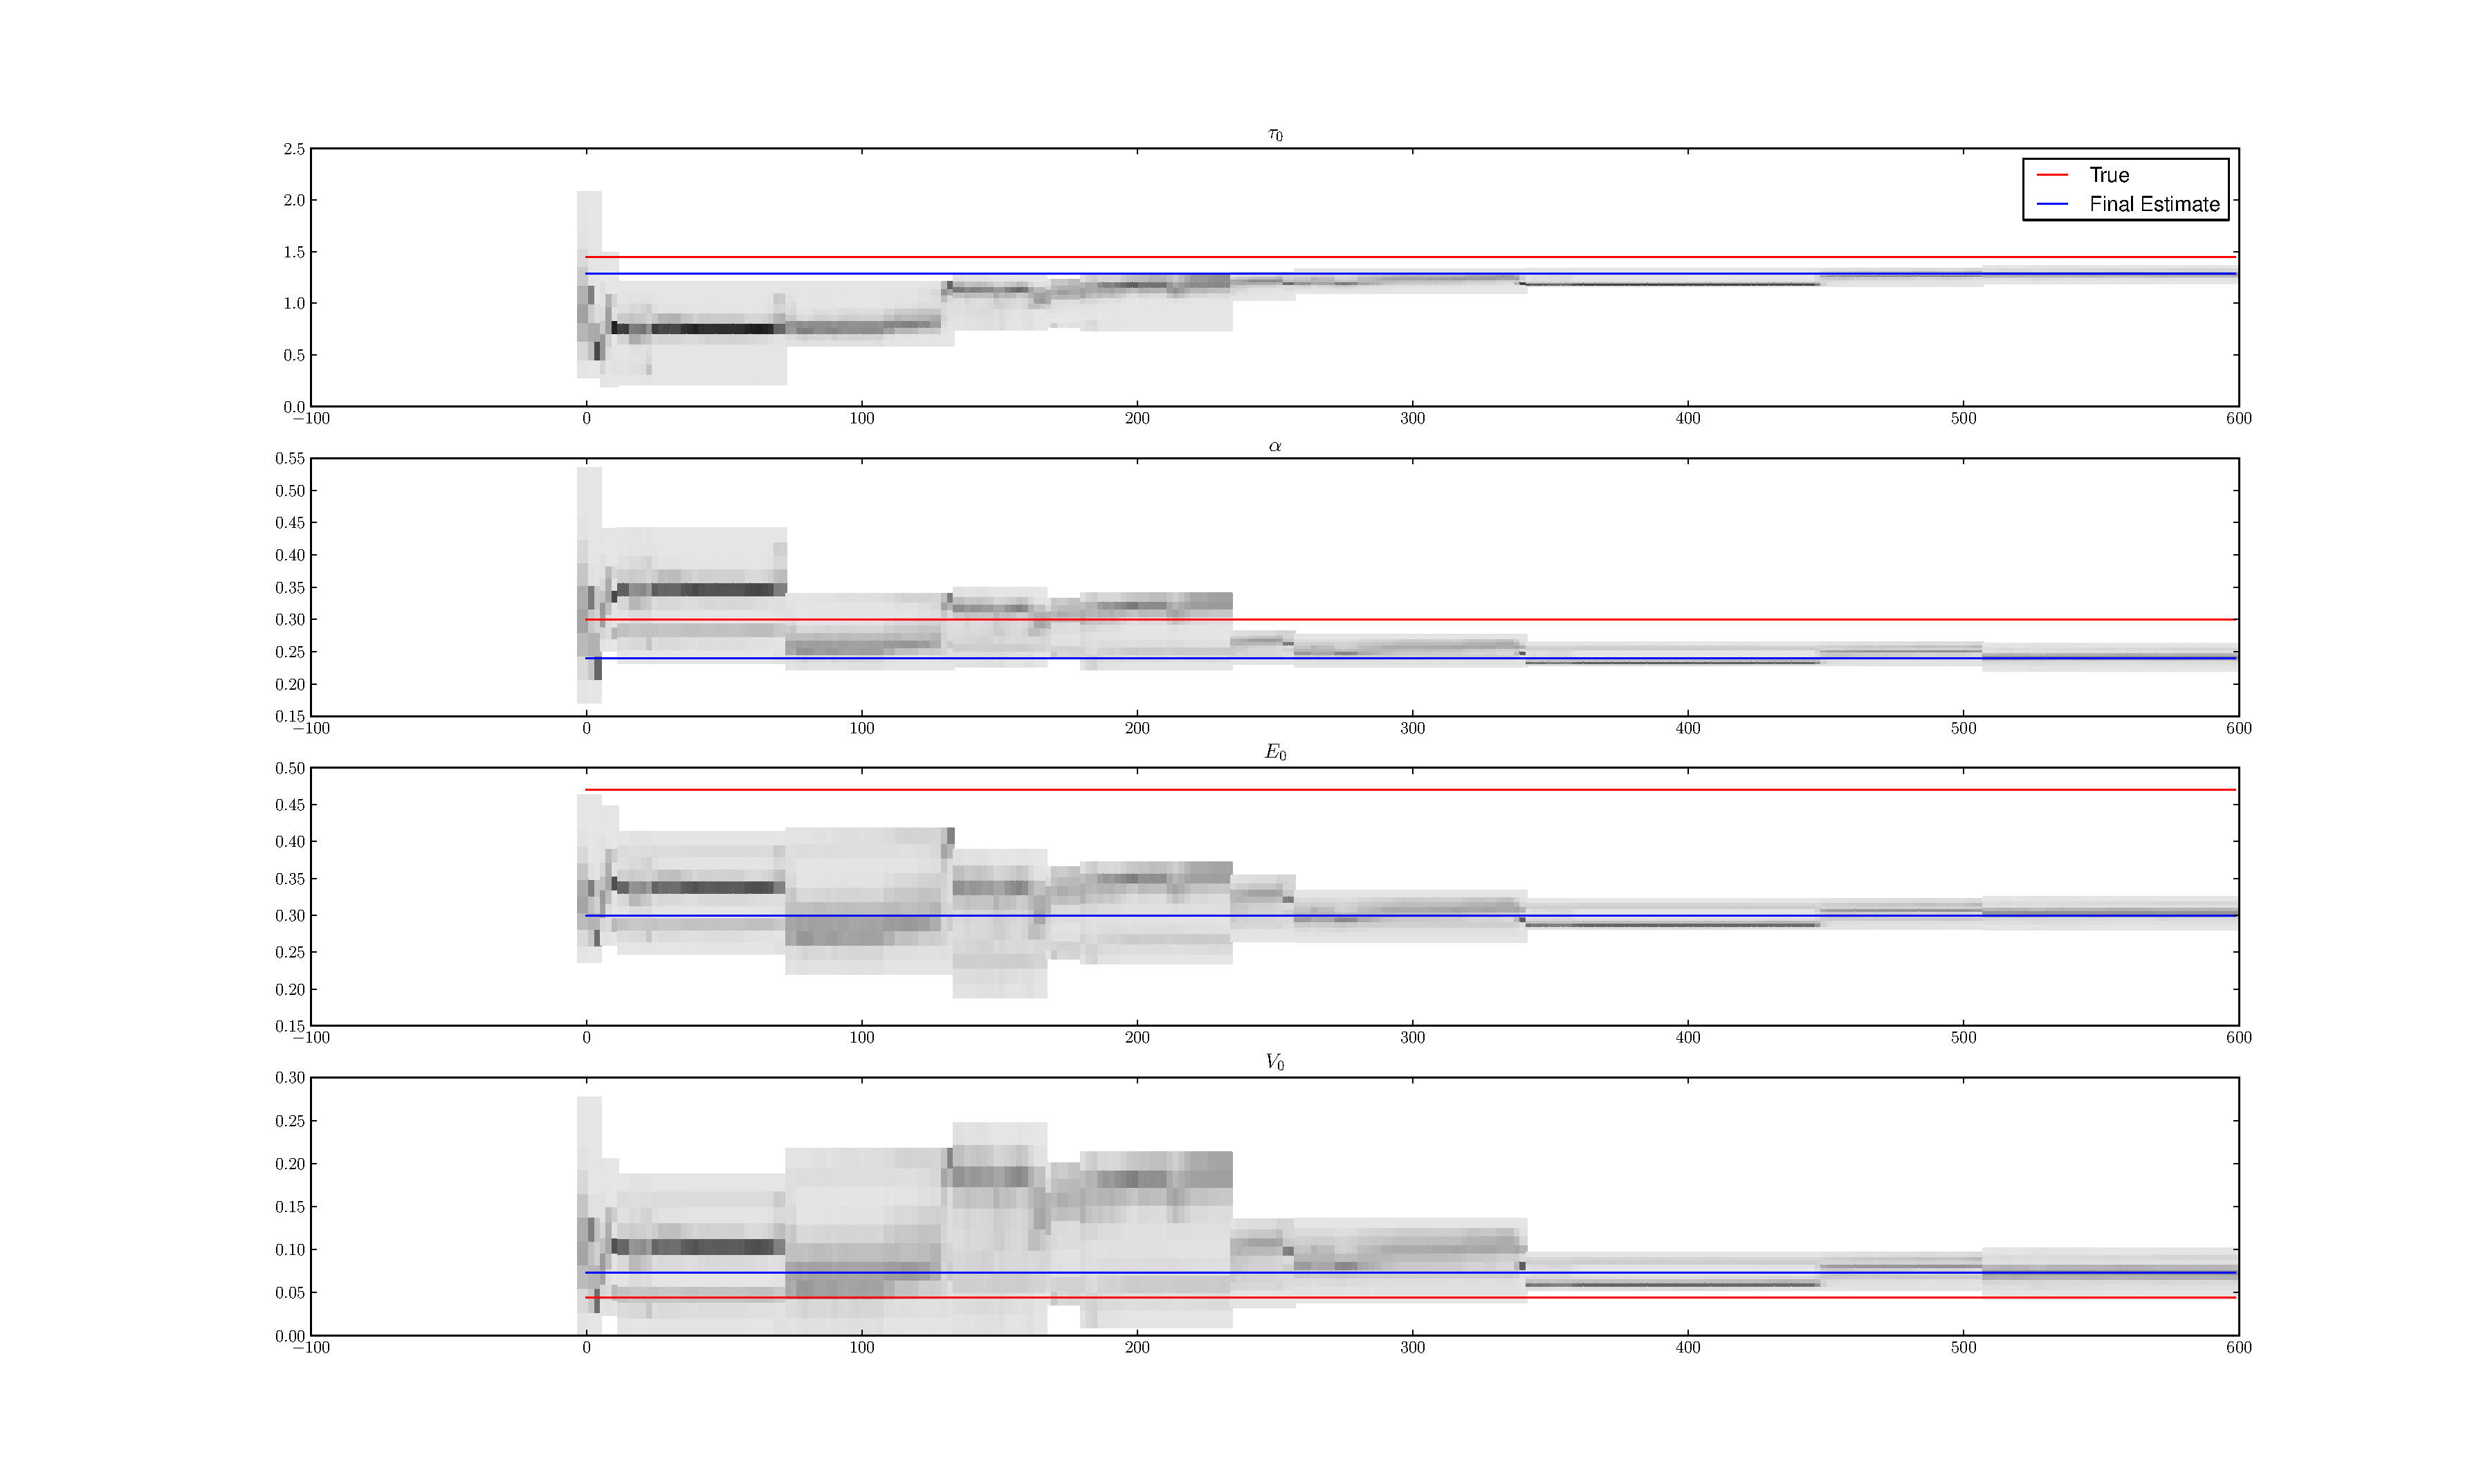
\includegraphics[clip=true,trim=6cm 3cm 6cm 3cm, height=9cm]{images/justbignoise_1}}\\
%\end{figure}
%\begin{figure}[H]
%\subfigure[$\tau_s$, $\tau_f$, $\epsilon$, $V$] 
%{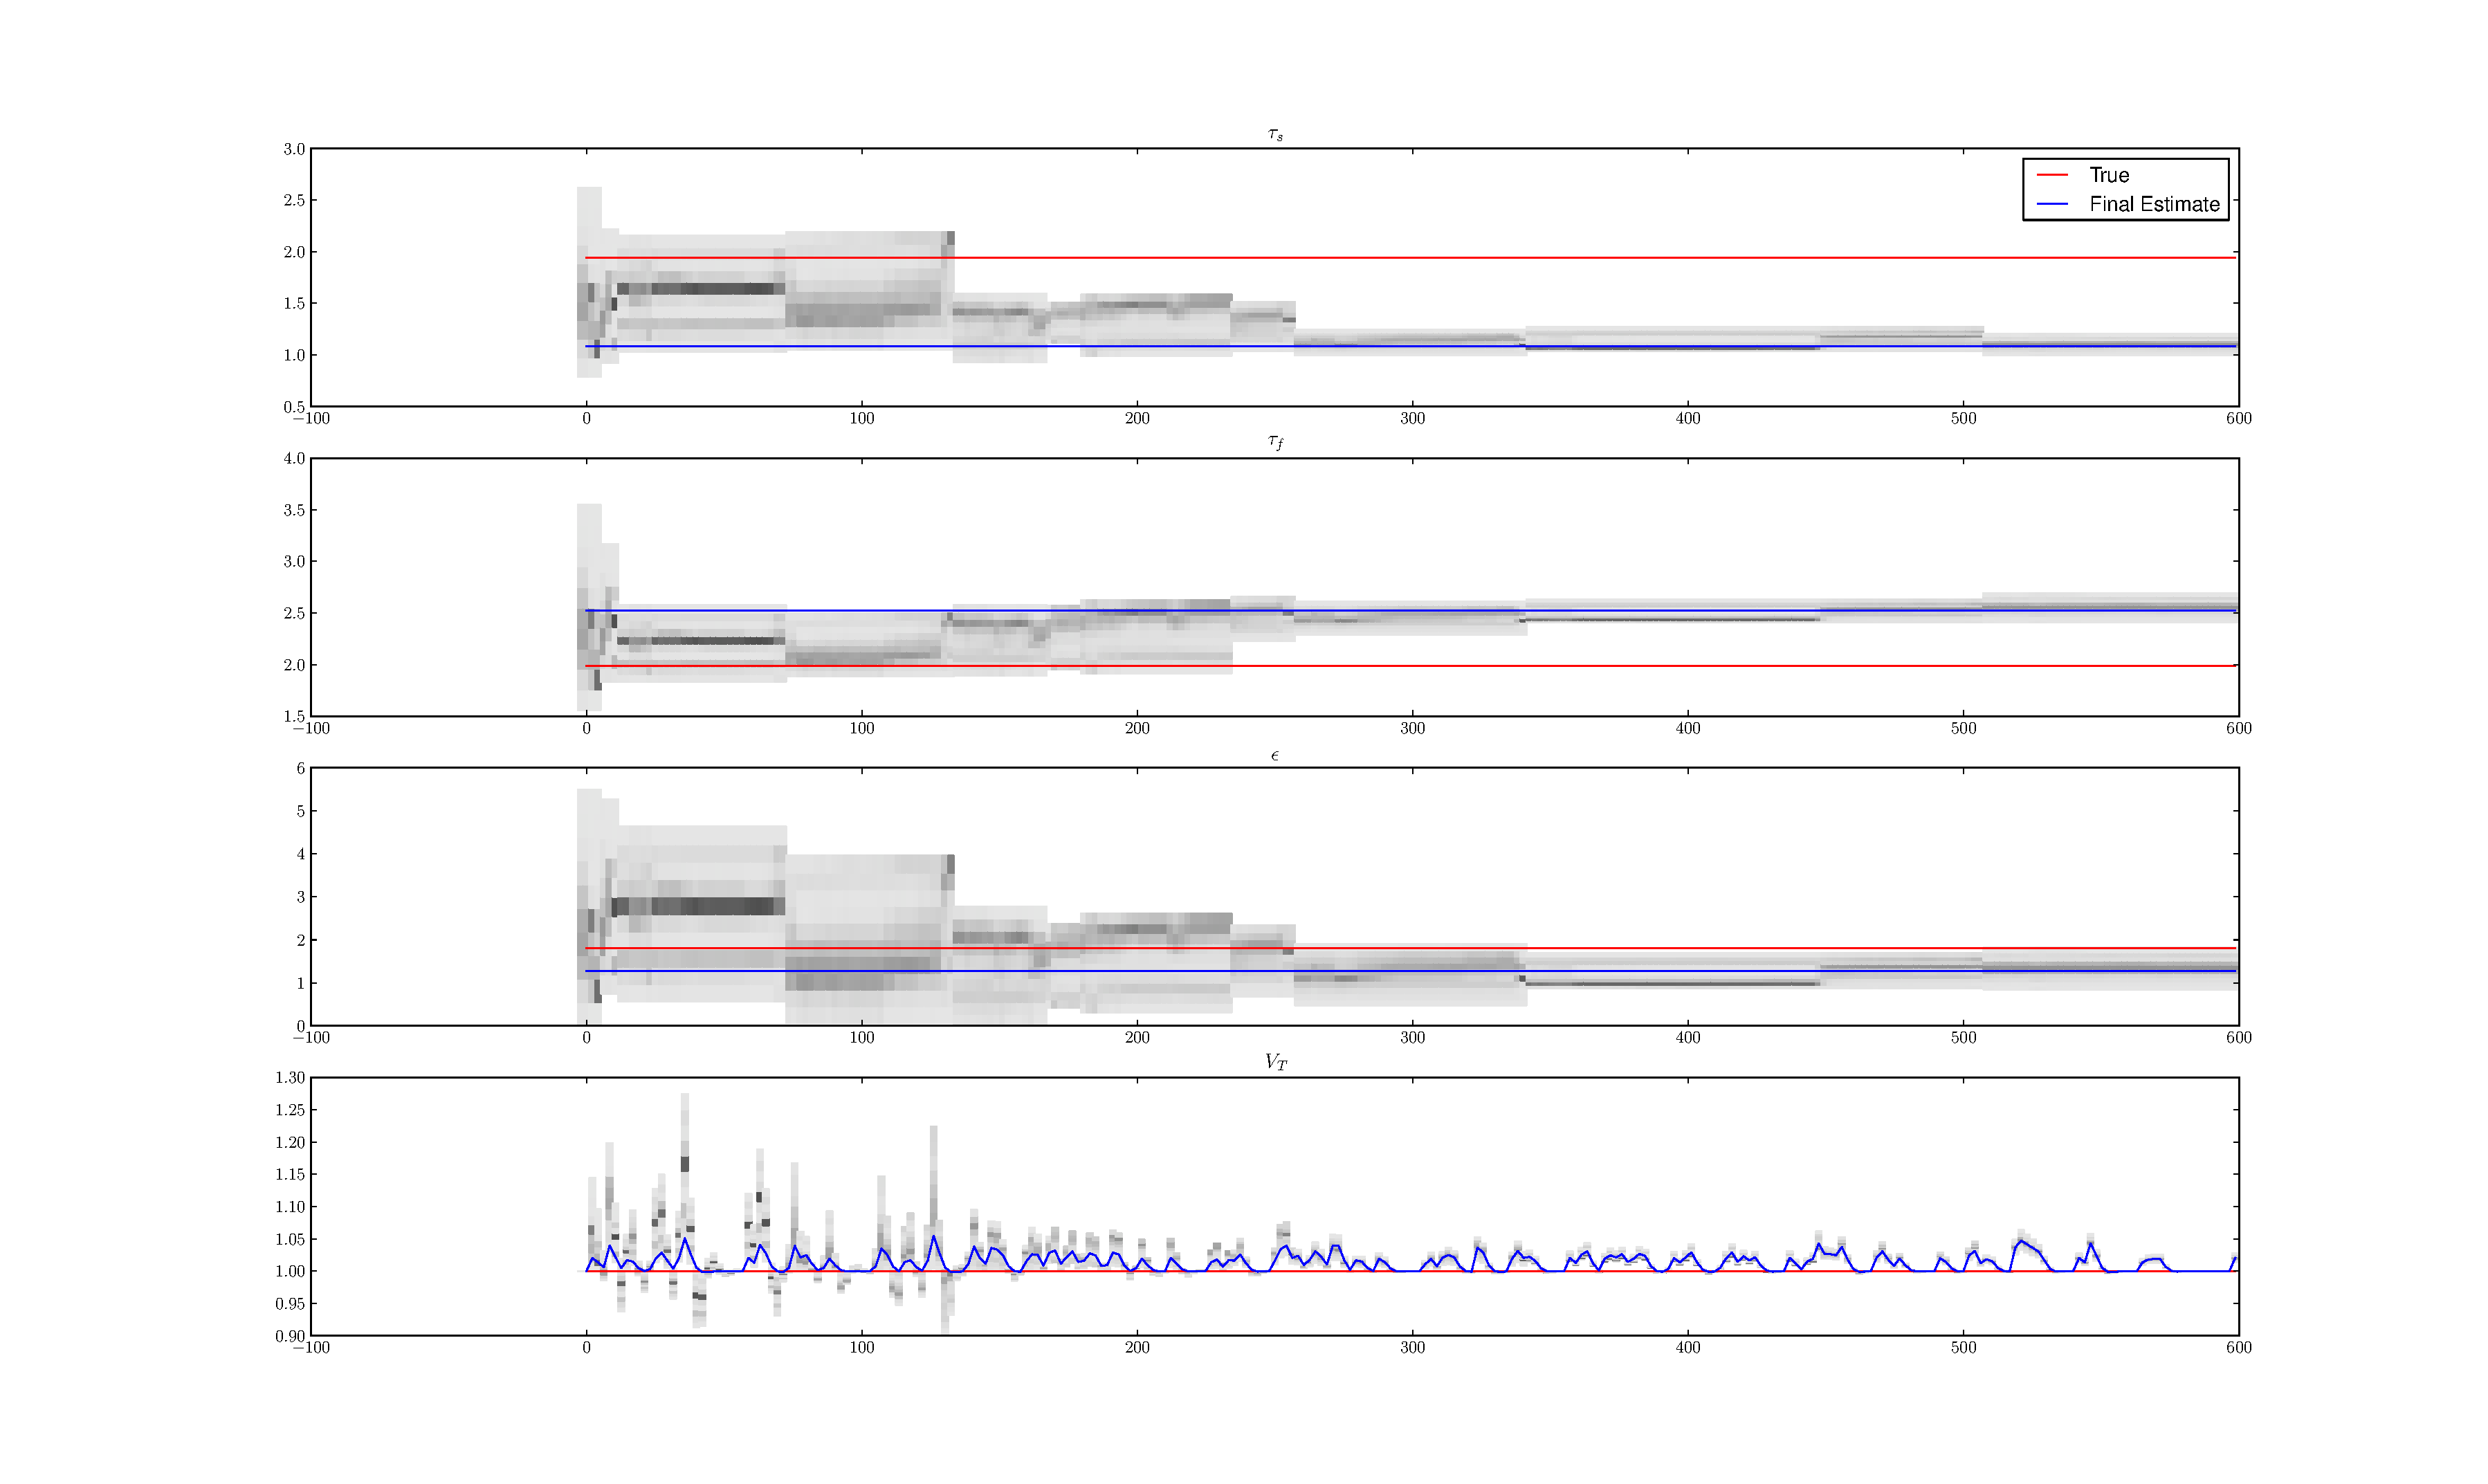
\includegraphics[clip=true,trim=6cm 3cm 6cm 3cm, height=9cm]{images/justbignoise_2}}\\
%\end{figure}
%\begin{figure}[H]
%\subfigure[$Q$, $S$, $F$, $BOLD$ ]
%{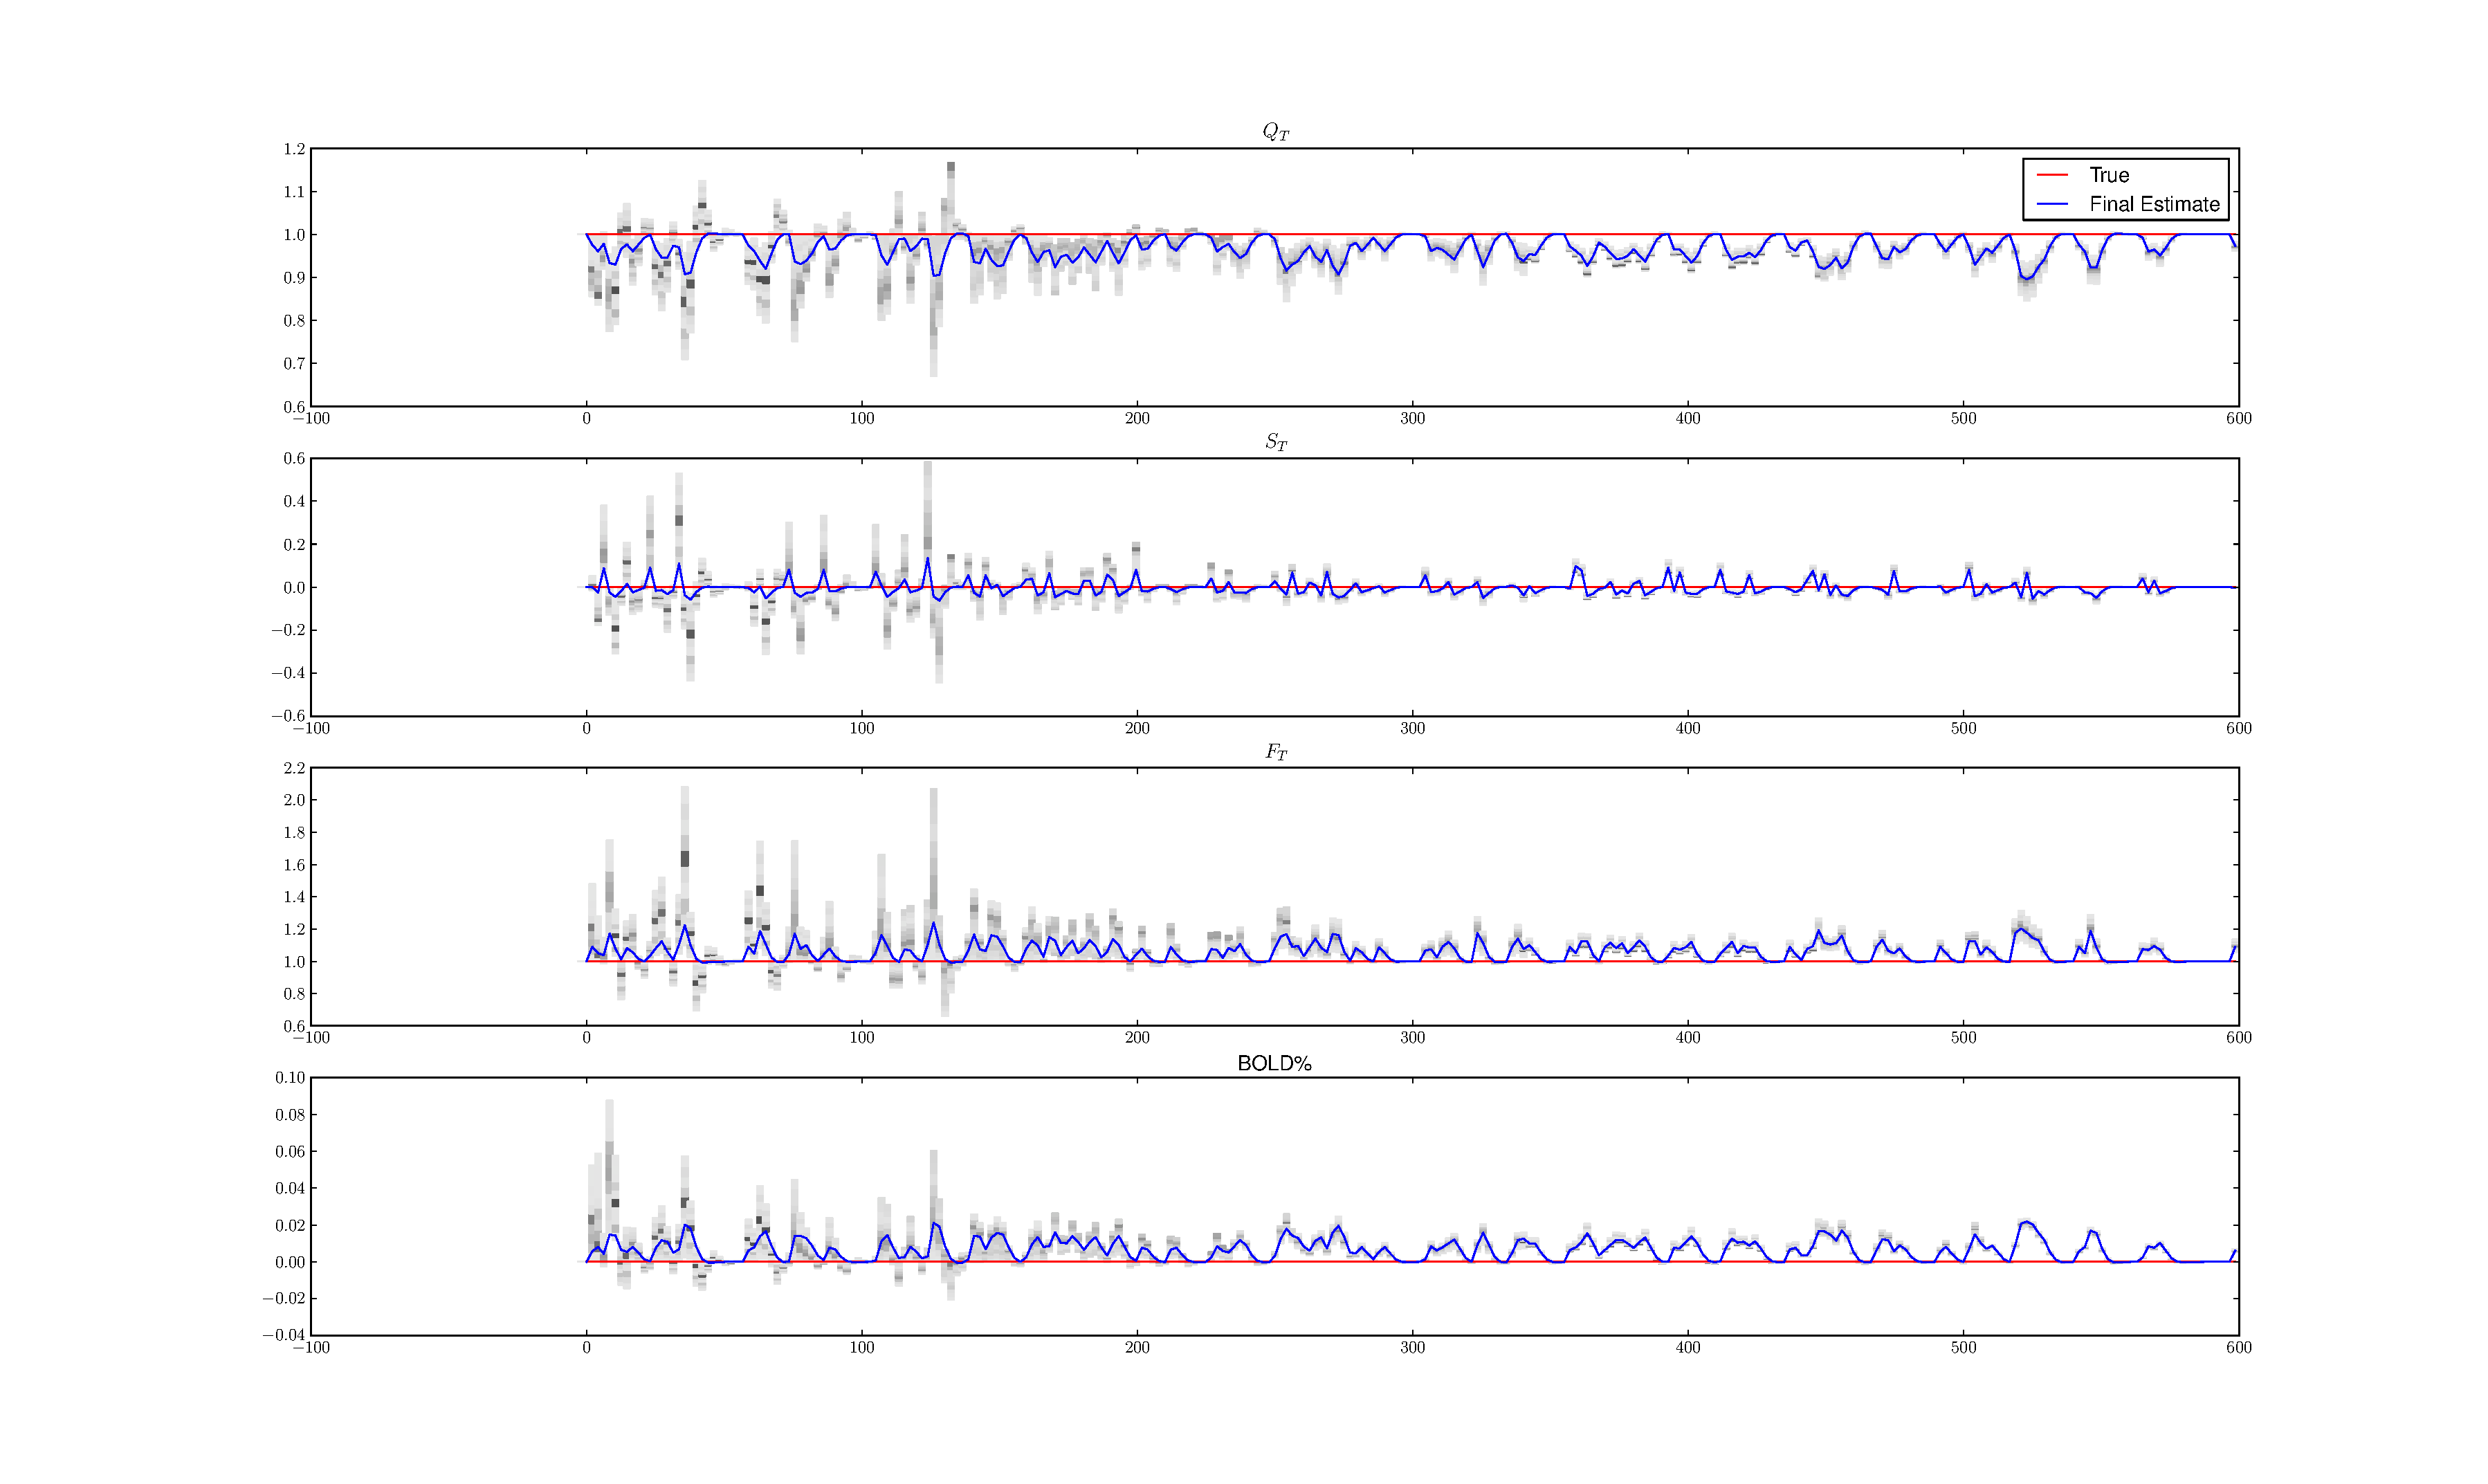
\includegraphics[clip=true,trim=6cm 3cm 6cm 3cm, height=9cm]{images/justbignoise_3}}
%\caption{Converging histogram for parameters when the signal consists purely of noise, with peaks comparable  to 
%the convential BOLD signal. ($\sigma_y = .01, \sigma_x = .005$). Same run as fit in \autoref{fig:justbignoise_fit_0}}
%\label{fig:JustNoiseConvergenceLarge}
%\end{figure}

From \autoref{fig:justbignoise_fit_0} it is clear that, despite the fact that the input 
is competely detached from the signal, a non-zero response by the particle filter does
lead to decreased residual. This is primarily due to the preprocessing which forces the signal to
have a non-zero mean. While this scheme could create a type of artificial activation for
the particle filter, in reality the residual will still be less than if the signal were left
with zero mean, and the particle filter stayed flat. At best the particle filter will 
over-smooth, estimating a centerline to noisy signal. In such a case
the residual will be the same as the alternative, although the mutual information will 
be different.

\subsection{Single Voxel Review}
\label{sec:SingleVoxelReview}
\begin{table}[t]
\centering
\begin{tabular}{|c | c | c | c | c | c | c | c | c |}
\hline 
& \multicolumn{4}{|c|}{Signal} & \multicolumn{4}{|c|}{No Signal}\\
\hline
& \multicolumn{2}{|c|}{Low Noise} & \multicolumn{2}{|c|}{High Noise} 
& \multicolumn{2}{|c|}{$\sigma_y = .001, \sigma_x = .0005$} 
& \multicolumn{2}{|c|}{$\sigma_y = .01, \sigma_x = .005$}\\
\hline 
& $M.I.$ & N. Res. &
  $M.I.$ & N. Res. &
  $M.I.$ & N. Res. &
  $M.I.$ & N. Res. \\
\hline       
\hline       
1 &   0.86687  &0.47801 &  0.09077  &1.03894 &  0.06326  &  1.29501 & 0.03024  &1.33641 \\
2 &   0.93975  &0.53177 &  0.13767  &0.95165 &  -0.01075  & 1.30175 & -0.02677 &1.33667 \\
3 &   0.82382  &0.5458  &  0.13505  &0.99539 &  0.02345  &  1.26287 & -0.0111  &1.15957 \\
4 &   0.94661  &0.49824 &  0.04341  &1.16129 &  -0.00906  & 1.43196 & 0.00147  &1.09988 \\
5 &   0.94281  &0.46805 &  0.13718  &1.03972 &  0.00663  &  1.25664 & -0.00204 &1.20107 \\
6 &   0.92539  &0.459   &  0.12337  &1.00214 &  -0.00816  & 1.2708 &  0.01775  &1.04589 \\
7 &   0.98892  &0.46096 &  0.15381  &1.08847 &  0.02664  &  1.15441 & 0.03163  &1.20543 \\
8 &   0.98796  &0.51838 &  0.11325  &1.05962 &  0.03285  &  1.27456 & 0.01951  &1.1225 \\
9 &   0.8804   &0.5253  &  0.09669  &1.0157  &  0.01628  &  1.32024 & 0.01039  &1.08637 \\
10 &  0.88721   &0.49211 & 0.18339  &1.18996 &  0.00407  &  1.34456 & 0.00508  &1.22135 \\
11 &  0.96644   &0.49092 & 0.10949  &0.95368 &  0.03323  &  1.32522 & -0.01284 &1.11737 \\
\hline                                                                         
mean &0.92329  &0.49714 & 0.12037   &1.04514 &  0.01622  &  1.29437 & 0.00576  &1.17568 \\
\hline                                                                           
min &  0.82382  &0.459   &  0.04341  &0.95165 & -0.01075  & 1.15441 & -0.02677 &1.04589 \\
\hline                                                                         
max &  0.98892  &0.5458  & 0.18339   &1.18996 & 0.06326  &  1.43196 & 0.03163  &1.33667 \\
\hline
\end{tabular}
\caption{Mutual Information and the normalized $\sqrt{MSE}$, 
    for signal/noise configurations.}
\label{tab:SignleVoxelActivationComparison} 
\end{table}

The first step in determining the validity of a model is to provide some order of quality
to rate the results by. Unfortunately, because of the variability in the signal levels the
raw $\sqrt{MSR}$ cannot perform this task. As demonstrated by \autoref{sec:PureNoiseLowMag},
a low residual does not necessarily indicate a good fit. 
Therefore, instead I  normalized the signal based on a value proportional to
the magnitude of the signal. Considering the tendency of FMRI noise to have large unexplainable
peaks and troughs, rather than using MAX and MIN values to estimate the scale of the 
signal, I used a robust estimator of 
scale; the Median-Absolute-Deviation (MAD). This is an estimator of the standard
deviation, and thus a good estimator of the scale of the input signal. 
The normalized residual values are 
shown in \autoref{tab:SignleVoxelActivationComparison}. A second potential method of 
gauging performance is mutual information. Mutual information is a method of measuring
the interdependence of two random variables. If two signals are truly independent,
then the mutual information will be zero. Although ideally suited to Bernoulli 
random variables where there are a finite number of options, by using histograms
it is possible to derive a joint distribution of two signals. The algorithm for 
mutual information is based on that joint distribution:
\begin{equation}
\sum_{x,y} p(x,y) \log_2\left(\frac{p(x,y)}{p(x)p(y)}\right)
\end{equation}
Unfortunately the number of bins causing bias in the output, thus to correct for this,
I subtracted the estimated bias:
\begin{equation}
\text{bias} = \frac{N_{bins}}{2Nlog(2)}
\end{equation}
where $N$ is the number of samples and $N_{bins}$ is the number of bins. For all
the mutual information estimates in this work 6 bins are used for the marginal
distribution of each signal. Additionally, throughout log base 2 will be used.
This leads to 36 total bins in the joint, so the bias is: 
\begin{equation}
\text{bias} = \frac{18}{N}
\end{equation}
After calculating the empirical mutual information, I subtracted the bias from
the estimated mutual information. Note that this can result in negative mutual
information, which should not technically be possible; so any negative mutual information
was taken as 0.

Comparing the results of \autoref{sec:HighNoise} and \autoref{sec:PureNoiseHighMag}, 
distinguishing between these cases with ether normalized residual or mutual information
is not clear cut. While the average mutual information is in fact more than 10 times
greater than the average mutual information in the two non-signal cases, the maximum
mutual information of the low noise/no signal case exceeds the minimum M.I. of the high noise/signal
case. The Low Noise/ signal determination is easier to make; given
the minimum mutual information is above $.8$ and the maximum normalized residual is below $.6$.
However, it is worth noting that the worst case scenario  for mutual information (maximum) in the
low noise/no signal case does not concur with the worse case (minimum) normalized residual. 
There is no reason why this has to be the case, it is beneficial. In
other words, if it were necessary to make a statement that
a particular voxel active or inactive; the accuracy would improve if both techniques
were used with loose restrictions, but a voxel would only be considered active if the
voxel passed both tests. 

There were two primary purposes of these tests. First, given the nature of monte-carlo
techniques it is important to ensure consistency of results. Although the parameter
sets were somewhat inconsistent, the quality of the fit was actually quite consistent
across eleven runs. The second purpose was of course to determine how the particle 
filter responded to different signal to noise ratios. 

\section{Multi-voxel Simulation}
To test the usefulness of the particle filter for I used a modified version of the FSL tool 
POSSUM to generate an entire FMRI image from a parameter map. The parameter map was generated
by taking an existing activation map and assigning discrete parameter sets to each region.
The result was a four dimensional (length x width
x height x parameter) image with spatially varying parameters. Possum was then modified
to take a parameter map and generate activation levels depending on the parameters at that
point. The patch for POSSUM will be made available. As an unfortunate side effect of 
not using Possums' original activation scale, I manually added 750 to the total level of
simulated Possum images. This is because the BOLD \% difference levels were in the range
of 50 - 100\% from the base, about 5 times as large as they should have been. Ultimately
this has no effect on the quality of the simulation and should not effect the 
underlying parameters (other than perhaps $\epsilon$ and $V_0$). 
Also worth noting is that the noise level was set to an SNR of 20, due to changes in the 
program the true signal-to-noise ratio was much lower, as seen in the fit in \autoref{fig:simslicefit1}.

\begin{figure}[H]
\centering
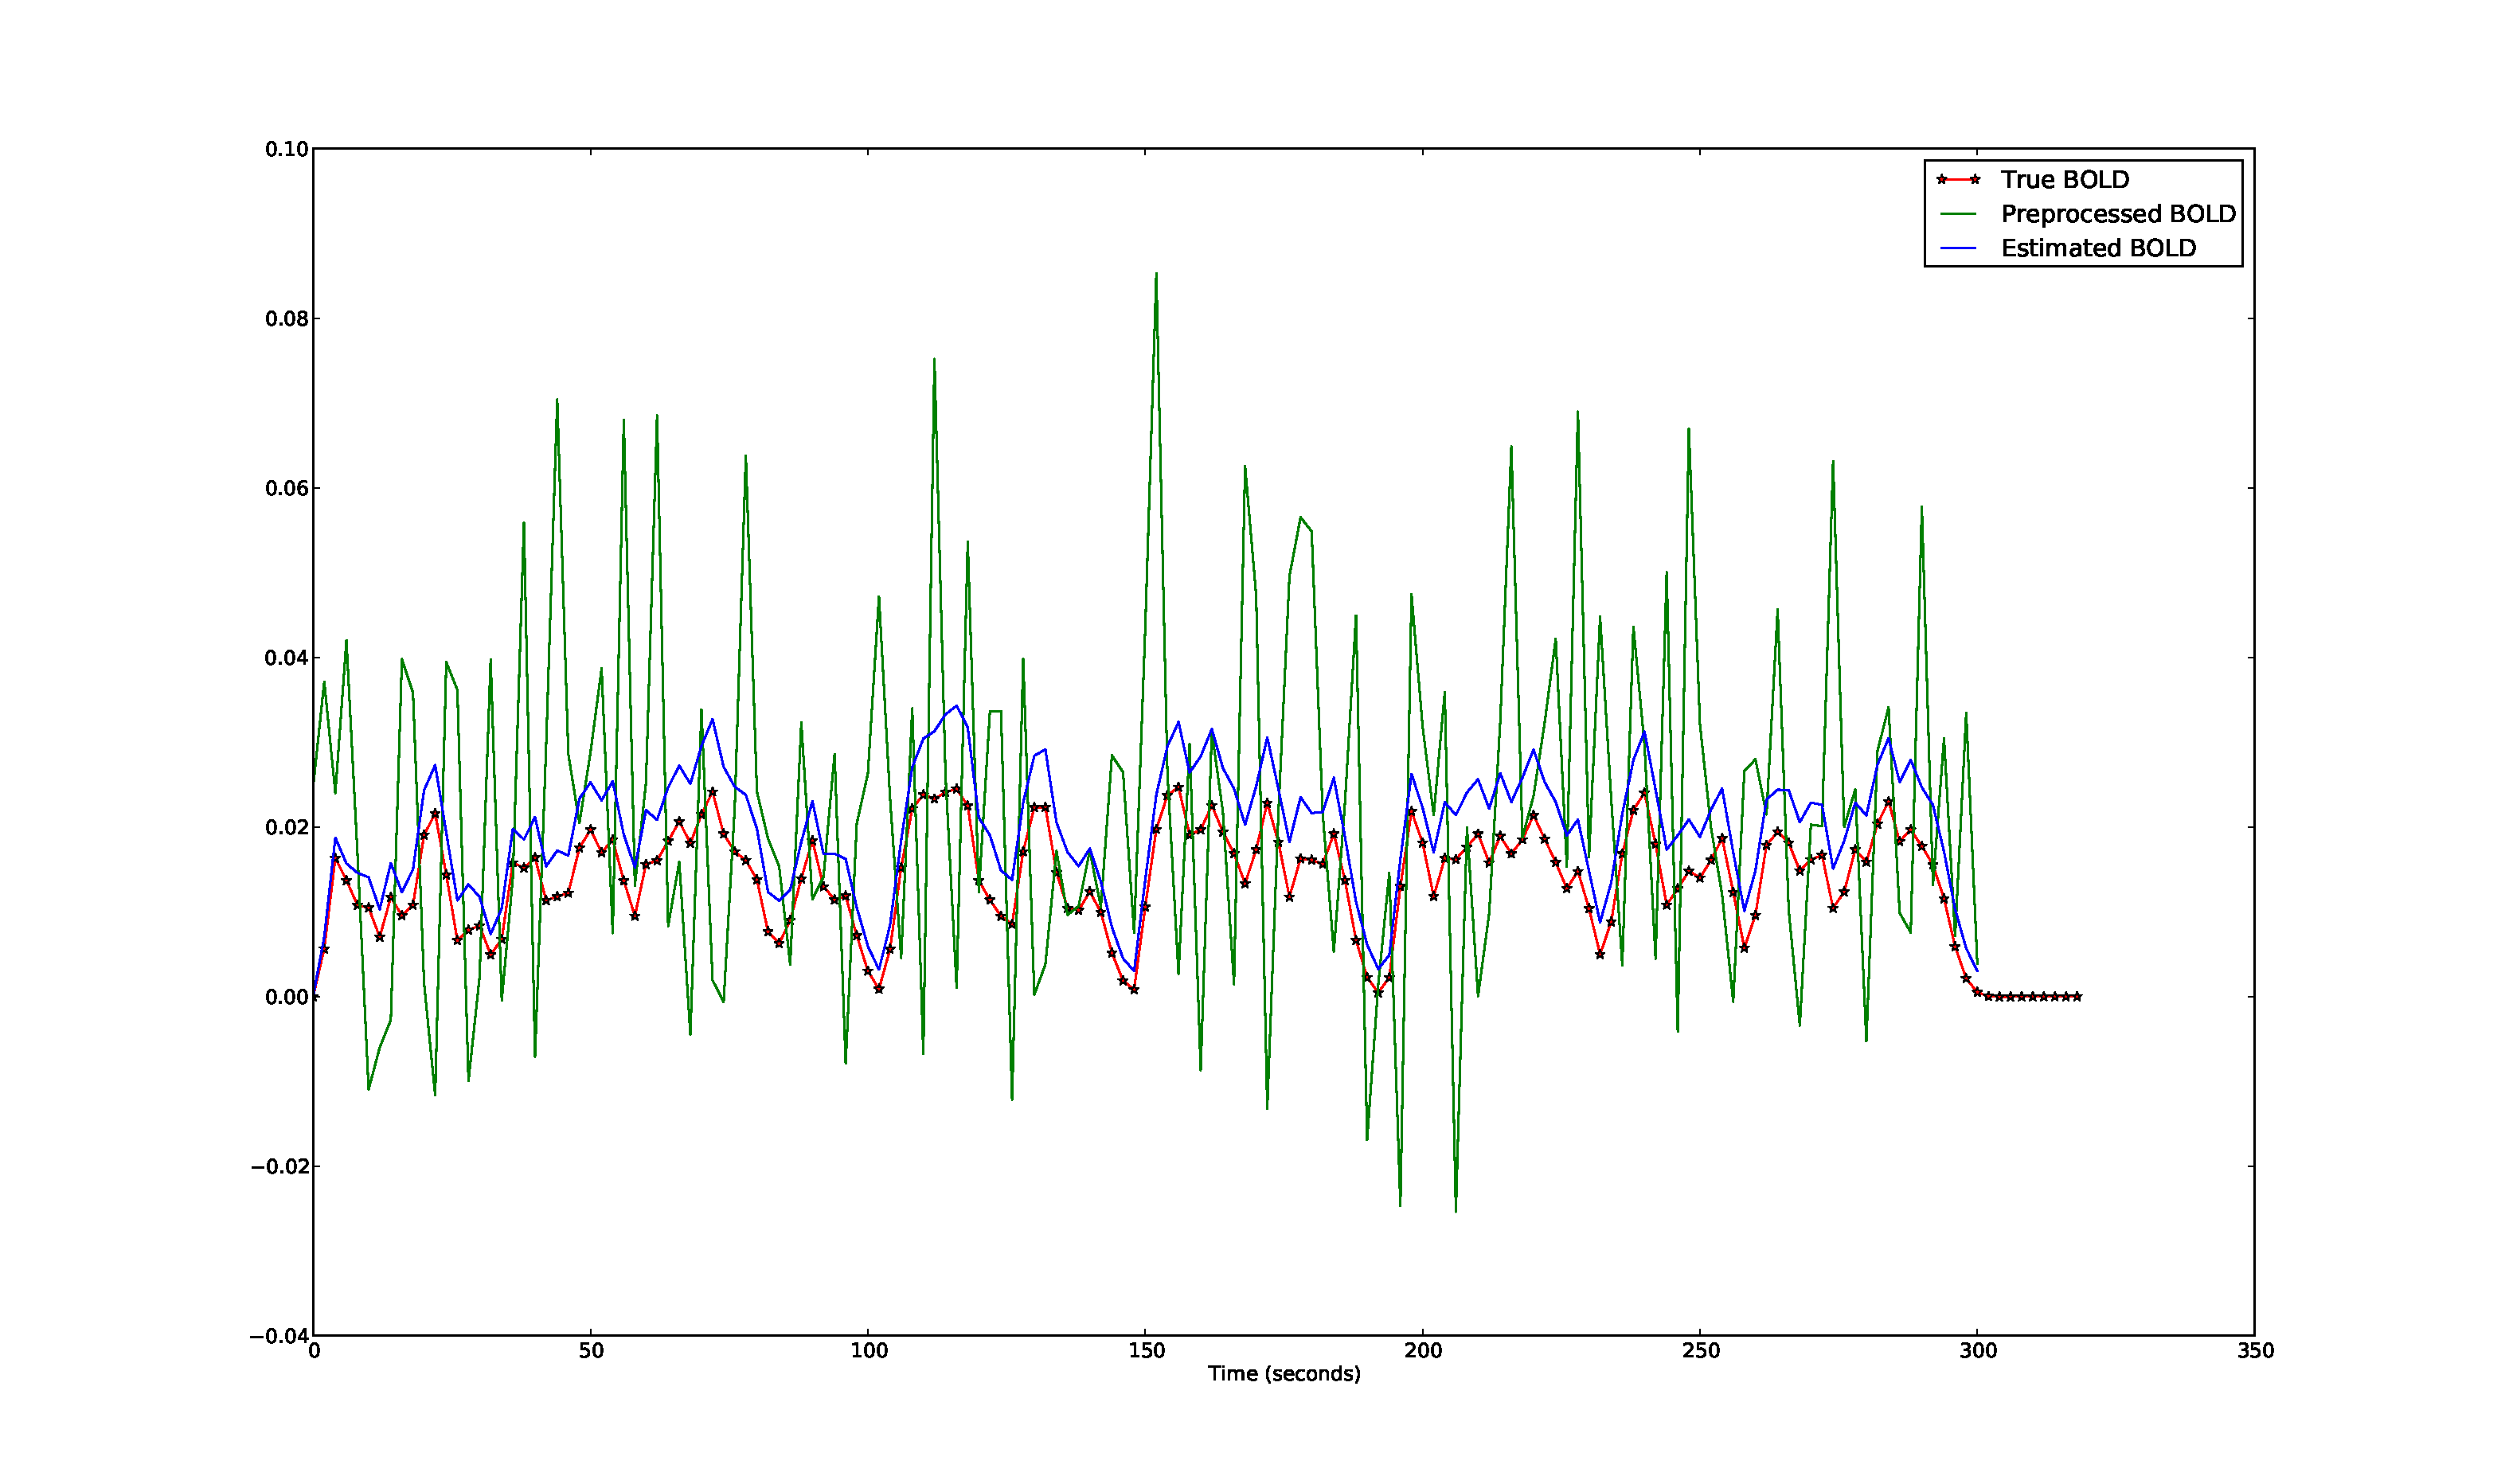
\includegraphics[width=15cm]{images/simslice_noise}
\caption{A single time-series fit in the simulated slice.}
\label{fig:simslicefit1}
\end{figure}

For each time-series in the simulated FMRI image, the final \emph{static} parameters were saved
into a parameter map. This parameter map may then be compared to the map used to generate the 
simulated data; additionally a new simulation using the calculated parameters may also be 
generated to test the difference in BOLD levels between the real parameters and the
estimated ones. Since it is the parameters are far from orthogonal 
(\cite{Deneux2006}), its possible that two sets of parameters are functionally equivalent,
despite large difference. This way, a quantitative difference between the two parameter sets 
was found.

\begin{figure}[H]
\centering
\subfigure[Region labels for simulated slice.]{
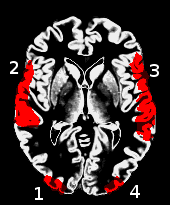
\includegraphics[height=9.5cm]{images/simregions.png} \label{fig:simslice_mask} }
\subfigure[Grey matter map for simulate region.]{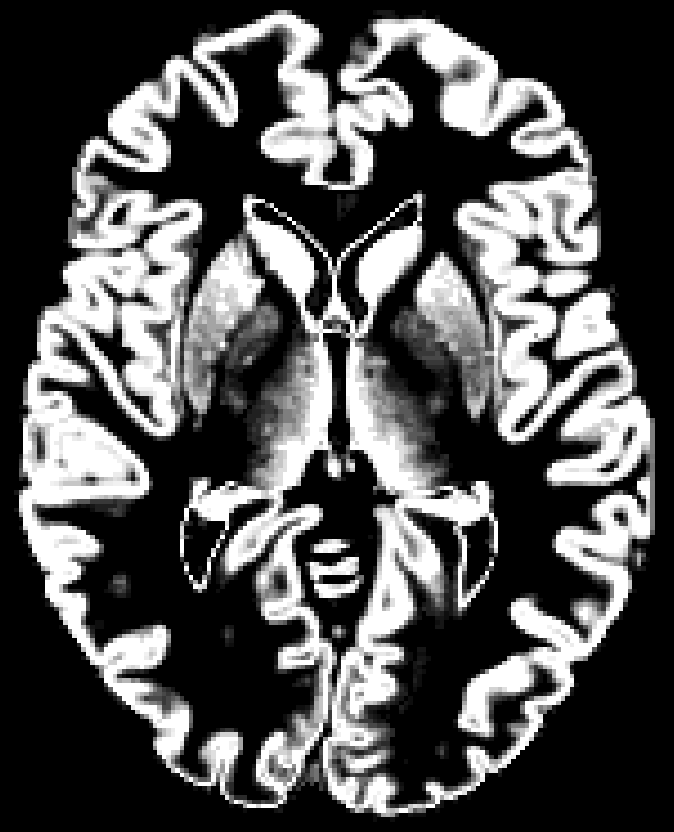
\includegraphics[height=9.5cm]{images/sim_gm}}
\subfigure[Residual Map. Scale is Normalized $\sqrt{MSE}$.]
{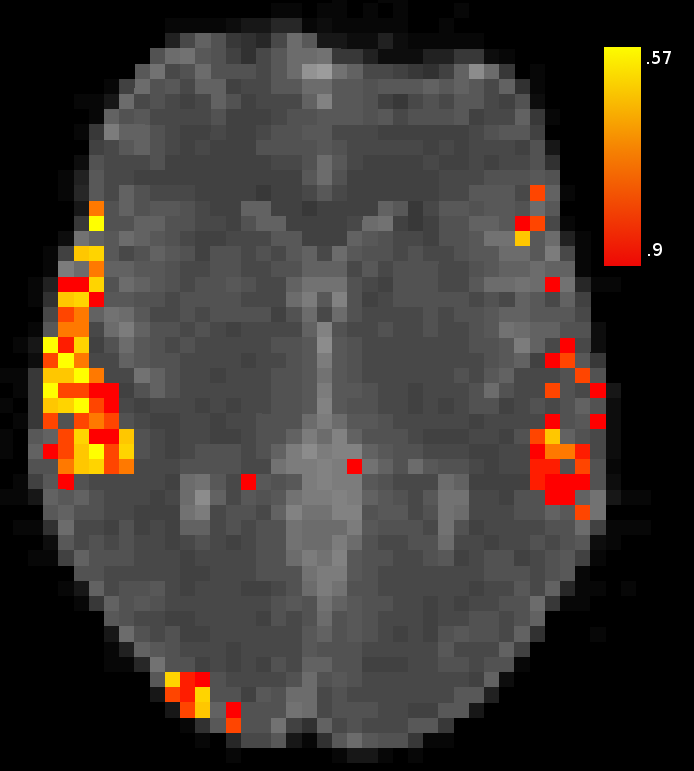
\includegraphics[height=9cm]{images/sim_hm}}
\subfigure[Mutual Information Map. Scale is bits.]
{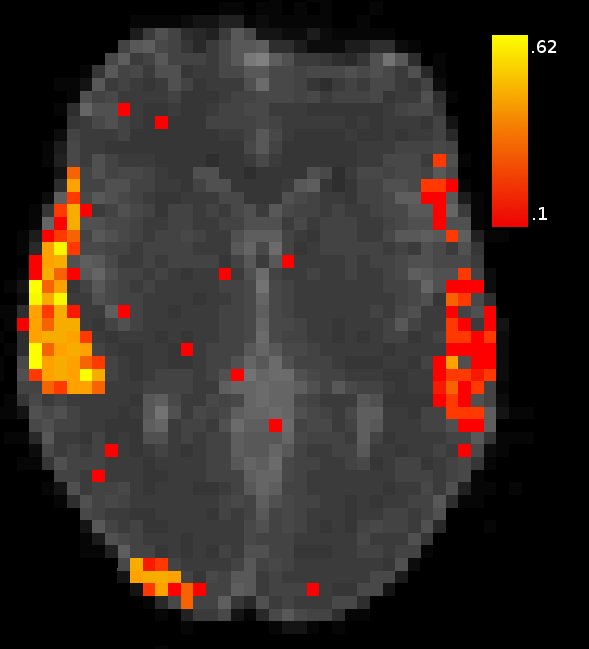
\includegraphics[height=9cm]{images/sim_hm_mi}}
\caption{Comparison of activation with greymatter, parameter regions.}
\label{fig:simslice_hm}
\end{figure}

The regions are numbered according to \autoref{fig:simslice_mask}; the parameters
for each region may be found in \autoref{tab:simsliceparams}. 

\begin{table}[t]
\centering
\begin{tabular}{|c |c | c | c | c | c | c | c |}
\hline 
Region & $\tau_0$ & $\alpha$ & $E_0$    & $V_0$    & $\tau_s$ & $\tau_f$ & $\epsilon$  \\
\hline 
1 & 1.454& .321& .369& .036& .994& 2.774& 1.348\\
2 &1.151& .353& .380& .026& 1.98& 2.333& 1.645 \\
3 &1.951& .317& .348& .027& 1.657& 3.719& .757 \\
4 &1.203 & .310& .326& .036& 2.168& 2.272& .086\\
\hline
\end{tabular}
\caption{Actual parameters for each regions in the simulated slice.}
\label{tab:simsliceparams} 
\end{table}
%last (bottom right), 1.203, .310, .326, .036, 2.168, 2.272, .086, 3.4, 1

Note that region 4 has a very low $\epsilon$. For this reason, the only areas
with significant estimates of the BOLD time series were 1,2 and 3. With
such a low $\epsilon$, region 4 was below the noise threshold. Notice that the
regions 1 2 an 3 stick out in both the $\sqrt{MSR}$ and the mutual information
map, indicating that the
particle filter was successful in matching those regions. 

\begin{figure} %bottom left
\centering
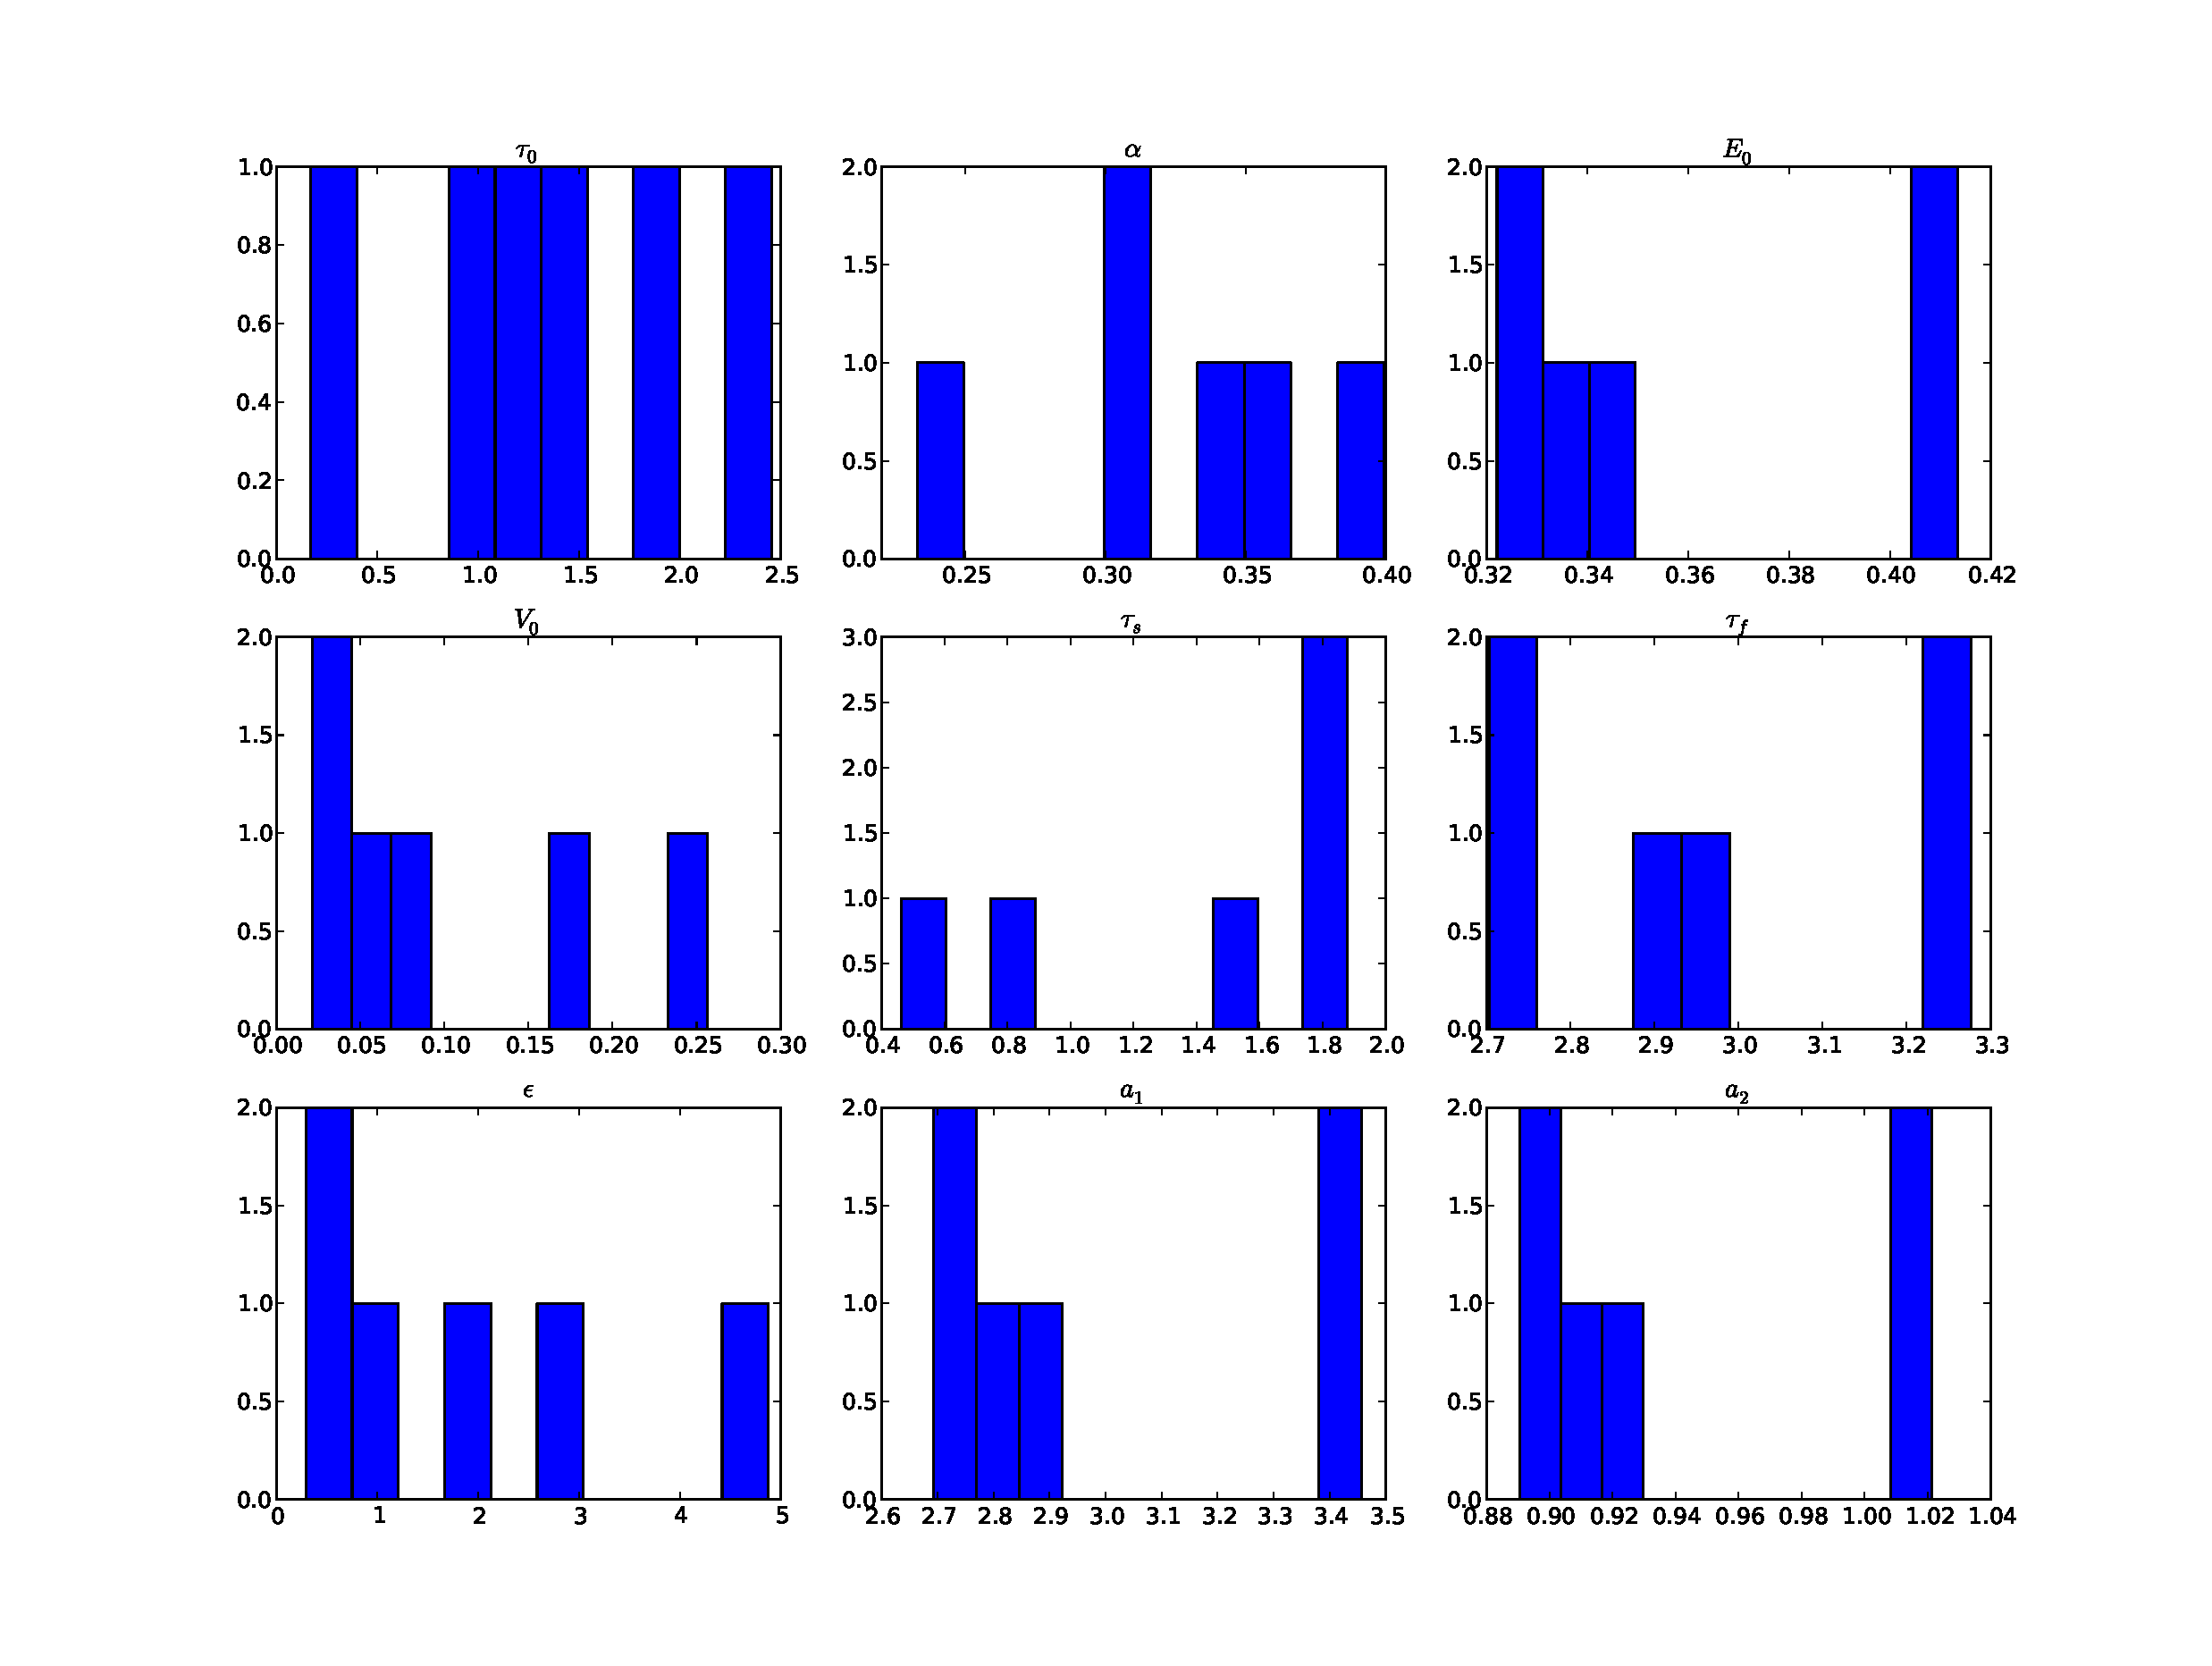
\includegraphics[clip=true,trim=2.5cm 2cm 2cm 1cm,width=15cm]{images/slicesim_hist1}
\caption{Histogram of estimated parameters in section 1 in voxels with mutual information greater
than $.14$}
\label{fig:slicesim_hist1}
\end{figure}

\begin{figure} %top left
\centering
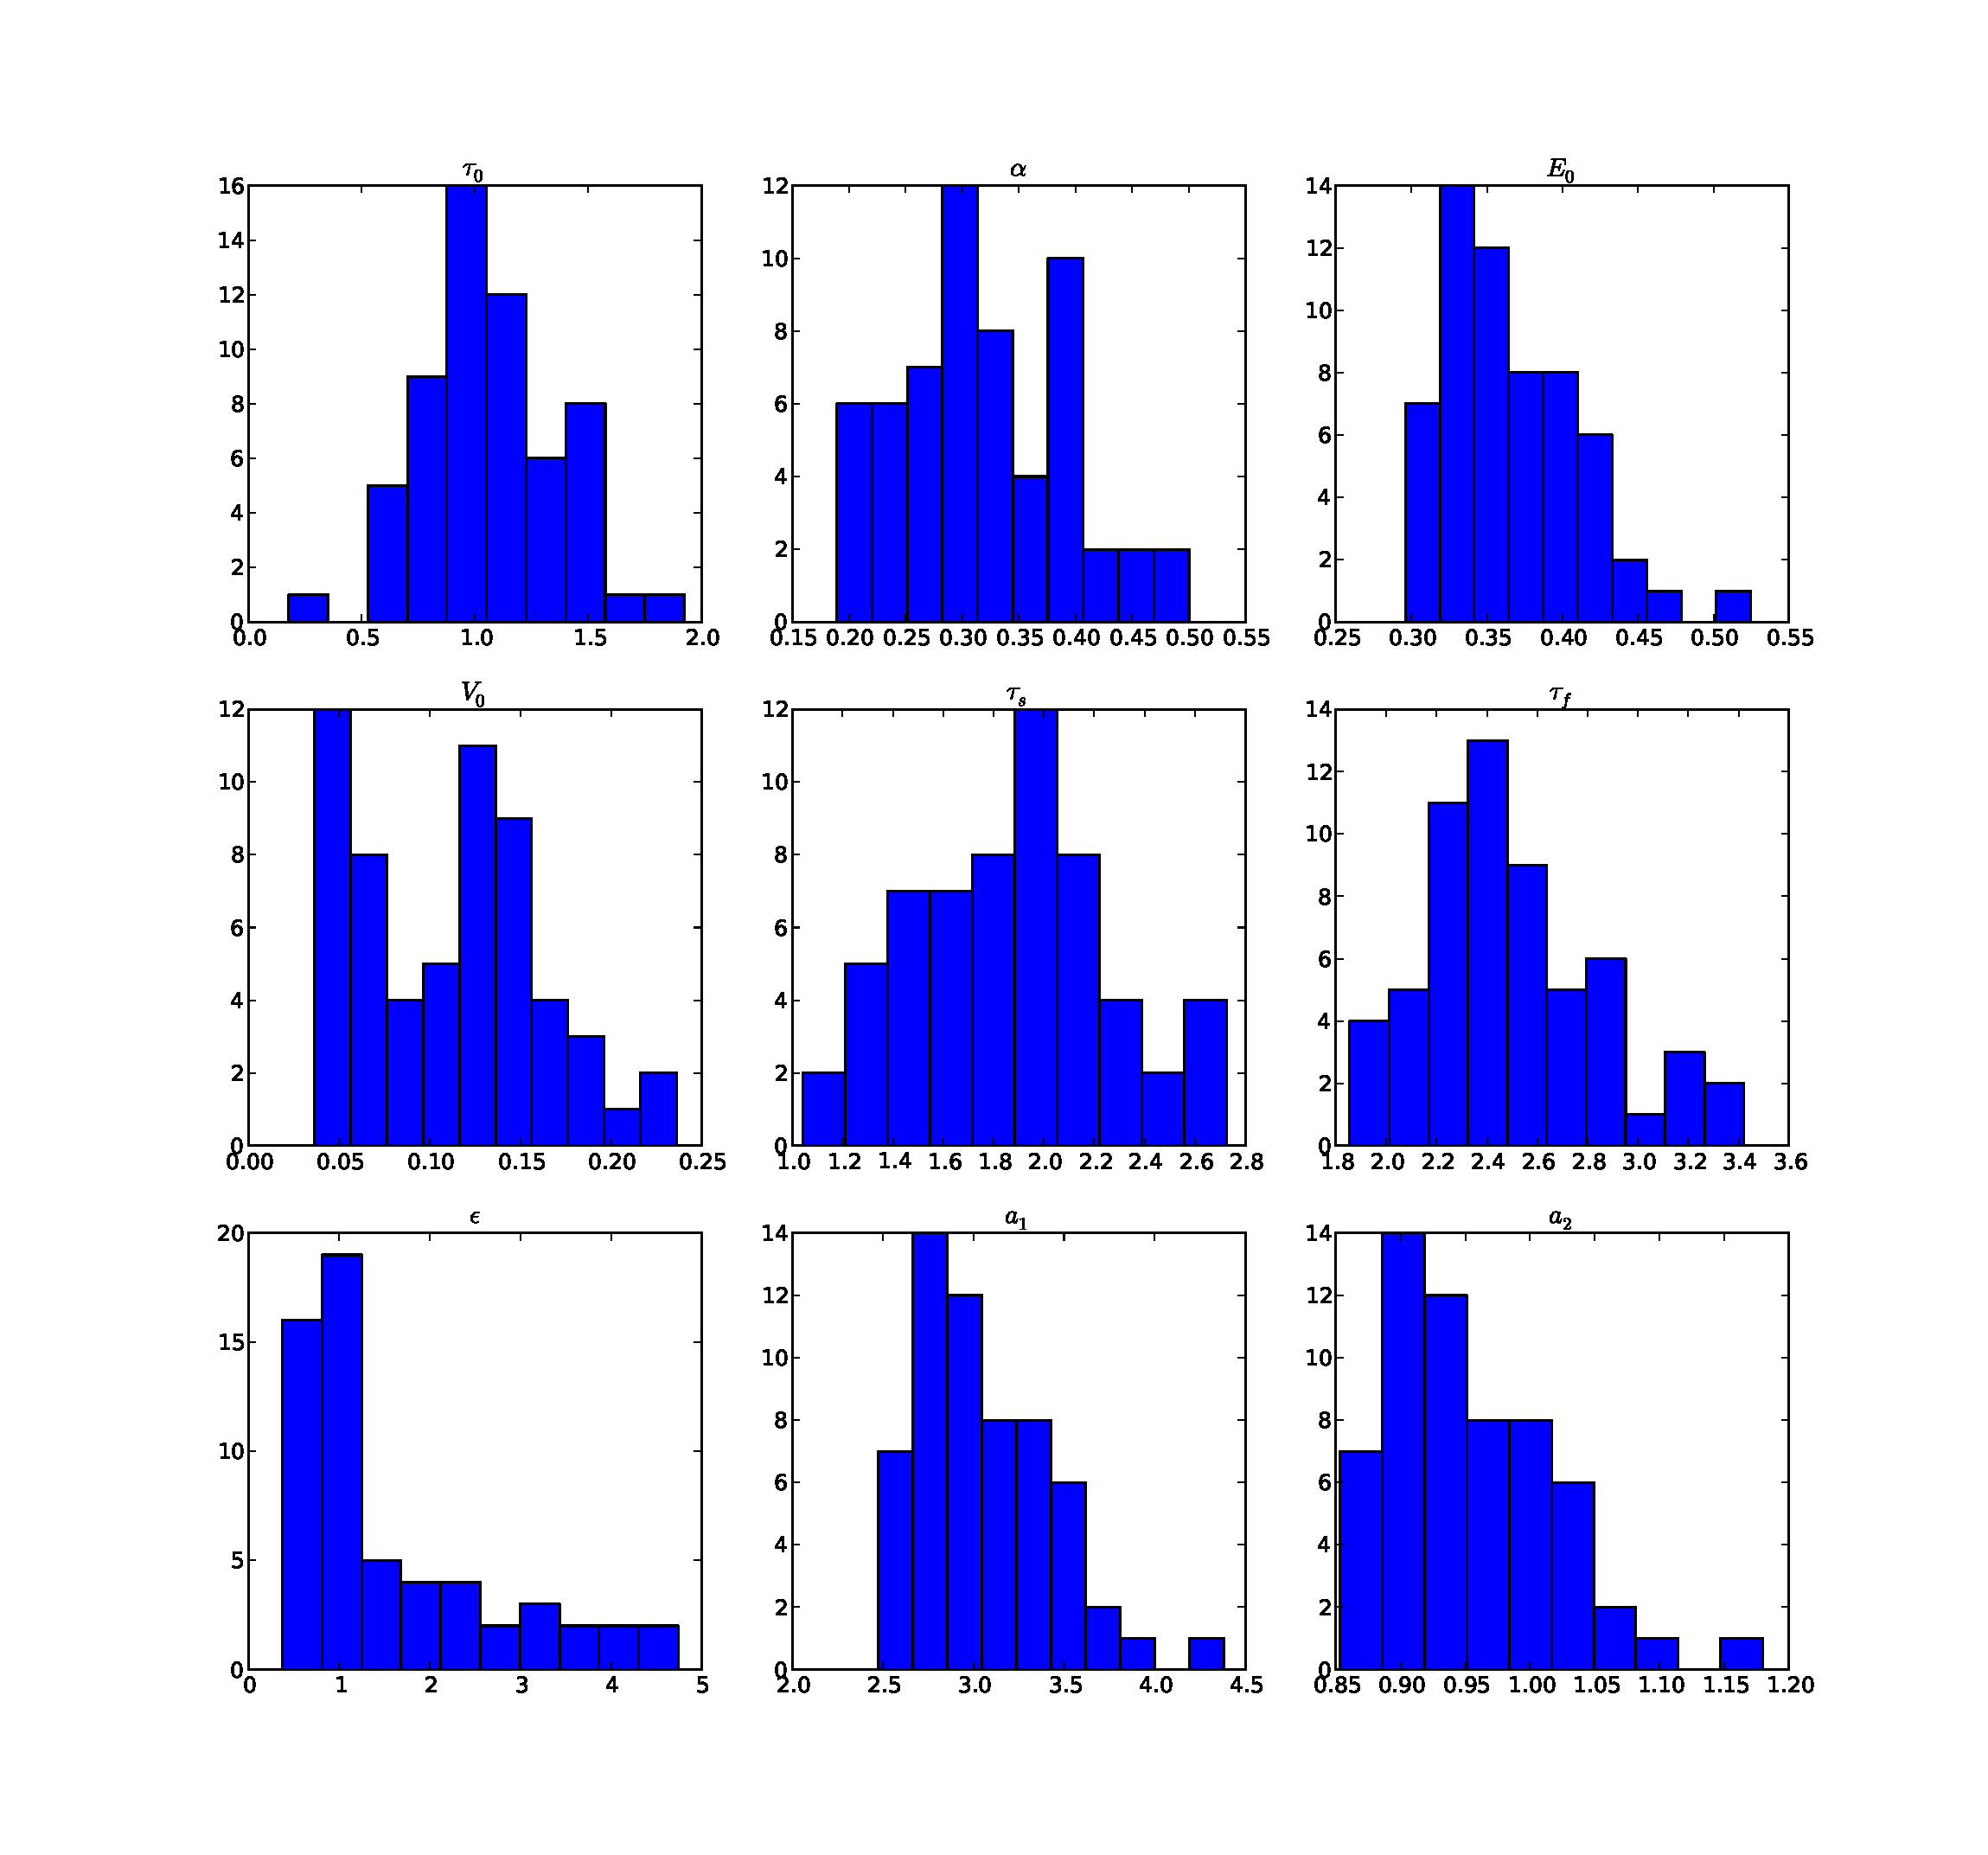
\includegraphics[clip=true,trim=2.5cm 2cm 2cm 1cm,width=15cm]{images/slicesim_hist2}
\caption{Histogram of estimated parameters in section 2 in voxels with mutual information greater
than $.14$}
\label{fig:slicesim_hist2}
\end{figure}

\begin{figure} %top right
\centering
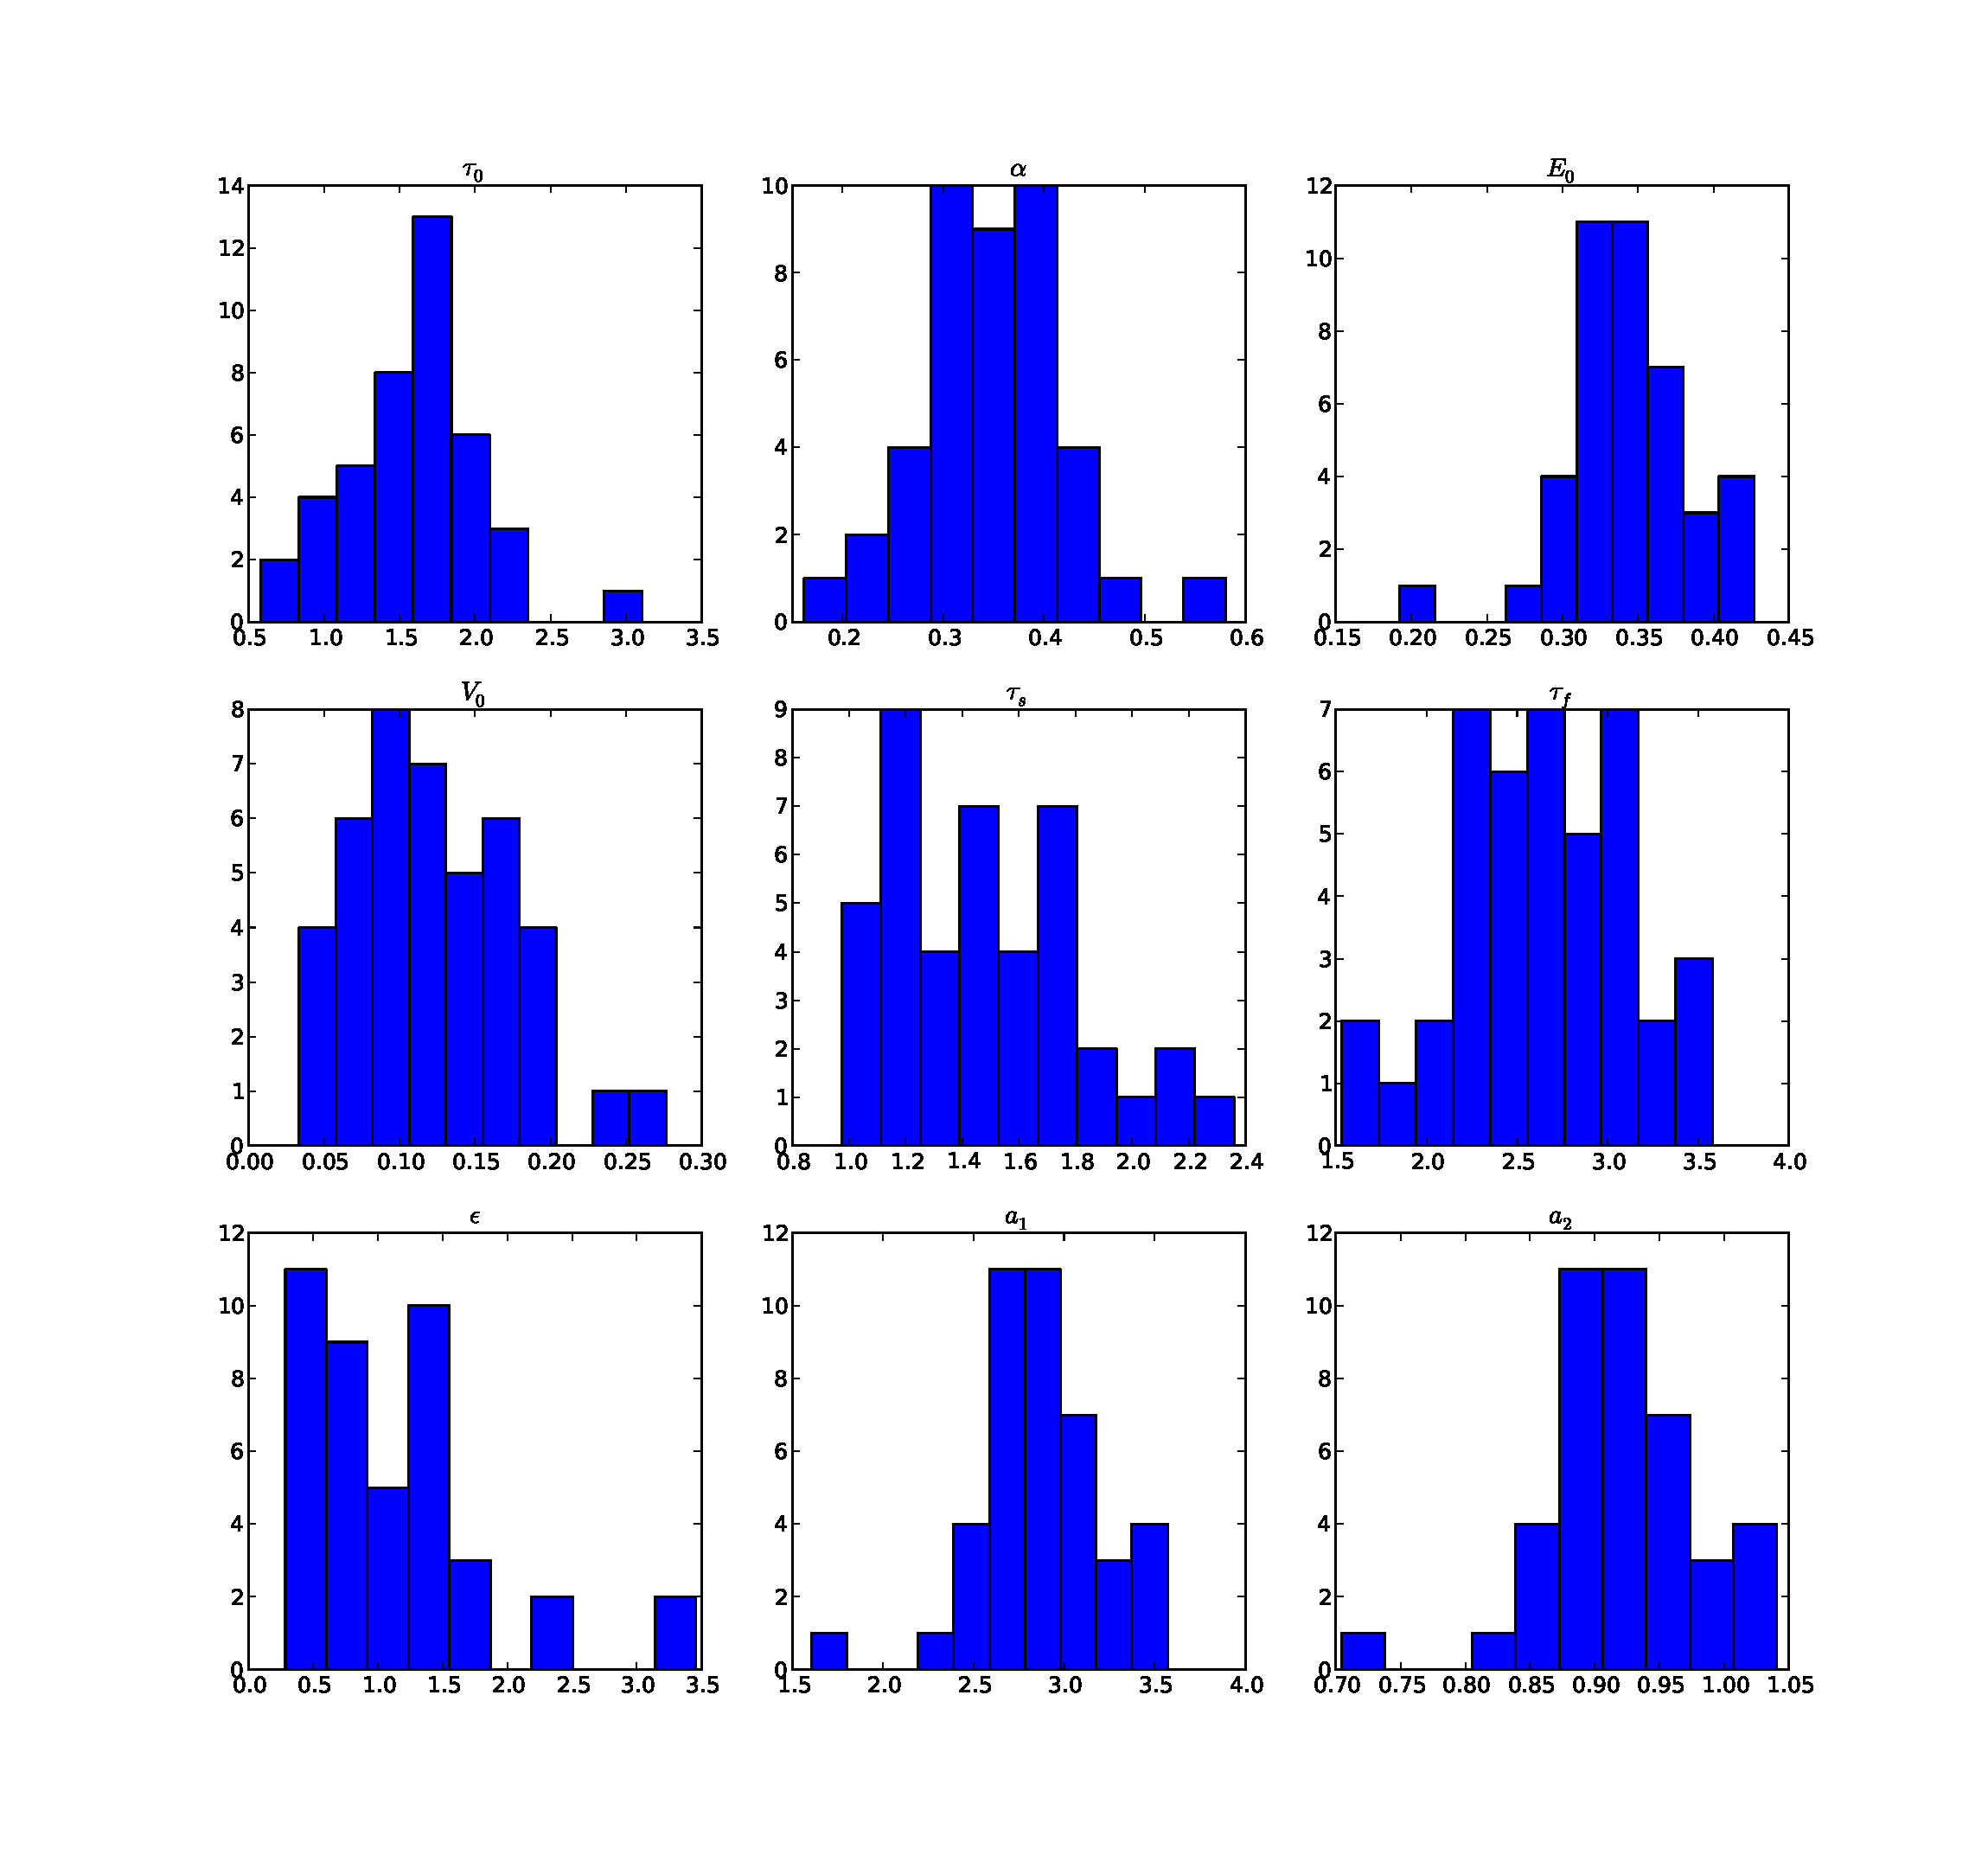
\includegraphics[clip=true,trim=2.5cm 2cm 2cm 1cm,width=15cm]{images/slicesim_hist3}
\caption{Histogram of estimated parameters in section 3 in voxels with mutual information greater
than $.14$}
\label{fig:slicesim_hist3}
\end{figure}

The histograms again demonstrate that a single point estimate of the parameters 
is elusive for the current model. However the data clearly show the power
of the particle filter at identifying regions of activation; which is usually
performed with statistical parametric maps. The thresholds applied to this
slice, both for mutual information and residuals is arbitrary, and needs further
research. Tighter thresholds removes the false positives present
in the images at the cost of false negatives. Interestingly the false 
positives present in the Mutual Information
map are different from those in the residual map. This furthers the argument from
\autoref{sec:SingleVoxelReview} for combining the two metrics to 
increase power. Although
at first glance it would appear that there are false negatives in the 
\autoref{fig:simslice_hm}; this is
not actually the case. POSSUM simulates different tissues, and white matter
does not typically  have a BOLD response. This is why there are holes in regions
2 and 3. These results certainly indicate that the particle filter is effective
at regressing against a noisy signal. Therefore the next section moves forward
with real FMRI data. 
